%  ========================================================================
%  Copyright (c) 1985 The University of Washington
%
%  Licensed under the Apache License, Version 2.0 (the "License");
%  you may not use this file except in compliance with the License.
%  You may obtain a copy of the License at
%
%      http://www.apache.org/licenses/LICENSE-2.0
%
%  Unless required by applicable law or agreed to in writing, software
%  distributed under the License is distributed on an "AS IS" BASIS,
%  WITHOUT WARRANTIES OR CONDITIONS OF ANY KIND, either express or implied.
%  See the License for the specific language governing permissions and
%  limitations under the License.
%  ========================================================================
%

% Documentation for University of Washington thesis LaTeX document class
% by Jim Fox
% fox@washington.edu
%
%    Revised 2020/02/24, added \caption()[]{} option.  No ToC.
%
%    Revised for version 2015/03/03 of uwthesis.cls
%    Revised, 2016/11/22, for cleanup of sample copyright and title pages
%
%    This document is contained in a single file ONLY because
%    I wanted to be able to distribute it easily.  A real thesis ought
%    to be contained on many files (e.g., one for each chapter, at least).
%
%    To help you identify the files and sections in this large file
%    I use the string '==========' to identify new files.
%
%    To help you ignore the unusual things I do with this sample document
%    I try to use the notation
%       
%    % --- sample stuff only -----
%    special stuff for my document, but you don't need it in your thesis
%    % --- end-of-sample-stuff ---


%    Printed in twoside style now that that's allowed
%
 
\documentclass[11pt, proquest]{uwthesis}[2020/02/24]
 
%
% The following line would print the thesis in a postscript font 

% \usepackage{natbib}
% \def\bibpreamble{\protect\addcontentsline{toc}{chapter}{Bibliography}}

\setcounter{tocdepth}{1}  % Print the chapter and sections to the toc
 

% ==========   Local defs and mods
%

% --- sample stuff only -----
% These format the sample code in this document

\usepackage{alltt}  % 
%\usepackage[version=4]{mhchem}
\usepackage{chemformula}
\let\ce\ch
\usepackage{xcolor}
\usepackage{graphicx}
\usepackage{booktabs}
\usepackage{caption}
\usepackage{subcaption}

\usepackage{textcomp}
\newcommand{\textapprox}{\raisebox{0.5ex}{\texttildelow}}

\usepackage{epstopdf}
\epstopdfDeclareGraphicsRule{.tif}{png}{.png}{convert #1 \OutputFile}
\AppendGraphicsExtensions{.tif}

\usepackage[backend=biber,style=chem-acs]{biblatex} % use autocite
\newenvironment{demo}
  {\begin{alltt}\leftskip3em
     \def\\{\ttfamily\char`\\}%
     \def\{{\ttfamily\char`\{}%
     \def\}{\ttfamily\char`\}}}
  {\end{alltt}}
 
% metafont font.  If logo not available, use the second form
%
% \font\mffont=logosl10 scaled\magstep1
\let\mffont=\sf
% --- end-of-sample-stuff ---
 
\addbibresource{all_references.bib}

\begin{document}
 
% ==========   Preliminary pages
%
% ( revised 2012 for electronic submission )
%

\prelimpages
 
%
% ----- copyright and title pages
%
\Title{Uses of the Many-Body Expansion for Studying Molecular Interactions and Driving Molecular Dynamics}
\Author{Joseph P. Heindel}
\Year{2022}
\Program{Department of Chemistry}

\Chair{Dr. Sotiris S. Xantheas}{}{}
\Signature{Dr. Anne B. McCoy}
\Signature{Dr. Charles T. Campbell}
\Signature{Dr. Stephanie Valleau}

\copyrightpage

\titlepage  

 
%
% ----- signature and quoteslip are gone
%

%
% ----- abstract
%


\setcounter{page}{-1}
\abstract{
\par The many-body expansion (MBE) is a method of decomposing any molecular property into contributions from the sub-systems of some total system. We focus on applying the MBE to detailed studies of the energy and forces of molecular clusters. In particular, we carry out the MBE up to full order for \ce{(H2O)7} and \ce{(H2O)_{10}} with increasingly complete basis sets. In doing this, we determine that the convergence of higher-order terms in the MBE depends sensitively on the presence of basis set superposition error (BSSE). Namely, the MBE for 3-body and higher terms in the energy is converged with an aug-cc-pVDZ basis set as long as a BSSE correction is included. If BSSE is ignored, however, the MBE oscillates from term to term and converges very slowly.

\par We carry out a similar analysis of ion-water clusters, \ce{Z^{+/-}(H2O)_{9}}, where \ce{Z^{+/-}}= \ce{Li^+}, \ce{Na^+}, \ce{K^+}, \ce{Rb^+}, \ce{Cs^+}, \ce{F^-}, \ce{Cl^-}, \ce{Br^-}, and \ce{I^-}. We verify the same conclusions about convergence of the MBE as for pure water clusters. Additionally, we find a remarkable linear anti-correlation between the total 2-body ion-water and 2-body and 3-body water-water interactions. This provides a quantitative measure of the extent to which hydrogen bond networks are disrupted by the presence of monoatomic ions. For both neutral and ion-water clusters, we find that the correlation energy makes less than 0.1\% total contribution to the energy at the 3-body and higher levels. That is, electron correlation only needs to be included at the 1- and 2-body levels to capture 99.9\% of the energy.

\par These detailed analyses lay the groundwork for a scheme in which high levels of electronic structure theory, such as MP2 and CCSD(T), can be used to drive the molecular dynamics of medium-sized systems without a major loss of accuracy. We first demonstrate that one can use the MBE to drive dynamics simulations with the MB-Pol water potential. These simulations result in the observation that the MBE is very slow to converge the angle between the full forces and forces calculated with the MBE. That is, the norm of the force vector converges at the 3-body level, but the angle between the full force vector and an approximate force vector is converged somewhere between the 4- and 6-body levels depending on how tight of convergence requirements one may have.

\par \textbf{STUFF ABOUT THE AIMD MBE-MD}
}
 
%
% ----- contents & etc.
%
\tableofcontents
\listoffigures
\listoftables  % I have no tables
 
%
% ----- glossary 
%
\chapter*{Glossary}      % starred form omits the `chapter x'
\addcontentsline{toc}{chapter}{Glossary}
\thispagestyle{plain}
%
\begin{glossary}
\item[argument] replacement text which customizes a \LaTeX\ macro for
each particular usage.
\item[back-up] a copy of a file to be used when catastrophe strikes
the original.  People who make no back-ups deserve
no sympathy.
\item[control sequence] the normal form of a command to \LaTeX.
\item[delimiter] something, often a character, that indicates
the beginning and ending of an argument.
More generally, a delimiter is a field separator.
\item[document class] a file of macros that tailors \LaTeX\ for
a particular document.  The macros described by this thesis
constitute a document class.
\item[document option] a macro or file of macros
that further modifies \LaTeX\ for
a particular document.  The option {\tt[chapternotes]}
constitutes a document option.
\item[figure] illustrated material, including graphs,
diagrams, drawings and photographs.
\item[font] a character set (the alphabet plus digits
and special symbols) of a particular size and style.  A couple of fonts
used in this thesis are twelve point roman and {\sl twelve point roman
slanted}.
\item[footnote] a note placed at the bottom of a page, end of a chapter,
or end of a thesis that comments on or cites a reference
for a designated part of the text.
\item[formatter] (as opposed to a word-processor) arranges printed
material according to instructions embedded in the text.
A word-processor, on the other hand, is normally controlled
by keyboard strokes that move text about on a display.
\item[\LaTeX] simply the ultimate in computerized typesetting.
\item[macro]  a complex control sequence composed of 
other control sequences.
\item[pica] an archaic unit of length.  One pica is twelve points and
six picas is about an inch.
\item[point] a unit of length.  72.27 points equals one inch.
\item[roman]  a conventional printing typestyle using serifs.
the decorations on the ends of letter strokes.
This thesis is set in roman type.
\item[rule] a straight printed line; e.g., \hrulefill.
\item[serif] the decoration at the ends of letter strokes.
\item[table] information placed in a columnar arrangement.
\item[thesis] either a master's thesis or a doctoral dissertation.
This document also refers to itself as a thesis, although it
really is not one.
 
\end{glossary}
 
%
% ----- acknowledgments
%
\acknowledgments{
  I wish to thank my wife, Leah Heindel, for showing me what it means to care deeply for others, for showing me how to balance passion with stability, and for always pushing me in better directions than the ones I choose for myself.
  
  Thank you to Daniel Schofield for introducing me to computational chemistry. You prepared me excellently for graduate school. Perhaps more importantly, you showed me that humility and scientific excellence are not mutually exclusive.
  
  Thank you to Anne McCoy for letting me hang around her group. I learned many things about science and being a scientist that I would not have figured out otherwise. You were also excellent at keeping my ego in check, which, on its own, is uncontrollably self-inflating.
  
  Finally, thank you to my advisor, Sotiris Xantheas. You have often treated me like family and I appreciate that immensely. You have given me every opportunity to succeed in science, so I hope I can make something of these favorable initial conditions.
  }

%
% ----- dedication
%
\dedication{\begin{center}Who to dedicate this to? 

Perhaps Silicon, without which computational chemistry would be much harder.\end{center}}

%
% end of the preliminary pages
 
 
 
%
% ==========      Text pages
%

\textpages



\chapter{The many-body expansion for aqueous systems revisited: I. Water-water interactions}

\section{Introduction}

\par The Many-Body Expansion (MBE) of the interaction energy of a system of n-fragments is a concept that has its origins in combinatorial mathematics and in particular the inclusion-exclusion principle, a counting technique introduced in the 1700s to obtain the number of elements in the union of finite sets.\autocite{roberts_applied_2009} It was first applied to water in 1970 by Hankins, Moskowitz, and Stillinger\autocite{hankins_water_1970} to obtain the 3-body contribution to the Hartree-Fock (HF) energy of a water trimer configuration consisting of a double donor, a double acceptor and a sequential water (but not to the trimer global ring minimum, which was missed in that study). We have subsequently used it in 1994 to decompose the energies of the minimum energy configurations of ring water clusters dimer through hexamer obtained at the second order Møller-Plesset (MP2) level of theory.\autocite{xantheas_ab_1994} That study also considered the effect of the Basis Set Superposition Error (BSSE) corrections\autocite{boys_calculation_1970, xantheas_importance_1996} to the individual many-body terms of these first few water clusters. A subsequent probe of the magnitudes of these terms for water clusters resembling bulk water configurations suggested that terms higher than two-body are less significant for configurations resembling bulk water, which have on the average two hydrogen bonds per water molecule.\autocite{xantheas_significance_1996} Finally, this analysis was reported for several low-lying minima of the first few water clusters in order to examine the variation of the magnitude of the many-body terms for different hydrogen bonding networks in order to investigate the origin of their relative stabilities.\autocite{xantheas_cooperativity_2000}
\par The interest in the many-body decomposition and in particular questions related to whether the magnitudes of the various terms exhibit a monotonic behavior, or the series converges and at which rank, stems from the need to understand and quantify the cooperative, non-additive (beyond two-body) interactions in water. The non-additive effects result in the shortening of the intermolecular O-O separation in the first few water ring cluster minima\autocite{xantheas_ab_1993, miliordos_optimal_2013} and the lengthening of the intermolecular O-H participating in the hydrogen bonds that causes a red shift in the positions of the corresponding OH vibrations with respect to those in the isolated gas phase monomer.\autocite{burnham_formation_2002} The general consensus that the series practically converges at the three-body term has fueled the development of a new generation of many-body interaction potentials for water such as the family of the Thole-type Models (TTM)\autocite{burnham_parametrization_1999, burnham_development_2002, burnham_development_2002-1, fanourgakis_flexible_2006, fanourgakis_development_2008} subsequent extensions and enhancements implemented in the Huang, Braams, Bowman (HBB2)\autocite{shank_accurate_2009, wang_towards_2010} and the Many-Body polarizable (MB-pol)\autocite{babin_toward_2012, babin_development_2013, babin_development_2013-1, babin_development_2014} models. These approaches are based on fitting separately the 1-, 2-, and 3-body potential energy surfaces (PESs) as well as the 1- and 2-body dipole moment surfaces (DMSs). The families of these potentials have demonstrated unprecedented accuracy for water\autocite{babin_development_2013, babin_development_2014, paesani_quantum_2007} and more recently for hydronium-water complexes\autocite{heindel_benchmark_2018}.
\par In recent years, the many-body expansion (MBE) has become a favorite tool for the accurate description of the molecular properties of water and molecules solvated in water. The MBE has provided an increasingly detailed understanding of the many-body convergence of properties of water ranging from the energies\autocite{xantheas_ab_1994, pedulla_theoretical_1998}, dipole moment and polarizability\autocite{medders_many-body_2013}, local and normal mode vibrational frequencies\autocite{heindel_origin_2018, howard_n-body_2013}, and forces\autocite{bates_efficient_2011, demerdash_convergence_2016, demerdash_assessing_2017}. Furthermore, the use of the MBE offers the possibility of employing highly accurate and computationally expensive \textit{ab initio} methods, such as Coupled Cluster with Singles, Doubles and perturbative estimate of Triples replacements [CCSD(T)] for the fragments of a molecular system, which is typically too large to be described at this level of theory. This, however, comes with the caveat that the number of sub-systems, for which calculations must be carried out, increases combinatorially with each term included in the MBE. Thus, as the system becomes large, it is not clear that using the MBE provides any real time savings unless the MBE is truncated at low-order. This is why it is important to understand when a sub-cluster can be neglected based on some distance or connectivity criteria.\autocite{cui_theoretical_2006, ouyang_when_2016} The MBE can also be used to decompose very large molecules, such as proteins, into subunits for smaller calculations.\autocite{mayhall_many-overlapping-body_2012, richard_many-body_2013} This scheme does provide a speedup relative to the full calculation, however these schemes typically involve splitting a system along a covalent bond, so the results can vary according to which subunits are chosen to reconstruct the whole system. Their flexibility exists in how these subunits are chosen, such as in the fragmentation of overlapping-bodies or in other fragmentation schemes of molecular clusters. These schemes have been unified in the so-called generalized MBE.\autocite{richard_generalized_2012}

\par There still exist outstanding questions regarding the convergence of the MBE for larger systems in regard to numerical precision, the overall accuracy that can be obtained for a given rank of the MBE\autocite{lao_understanding_2016, richard_understanding_2014} or the contribution of the correlation energy to the various terms. The numerical accuracy of the total k-body terms depends on both the size of the cluster (n) as well as the accuracy with which the energies of each of these terms are computed. The number of terms for expansion rank $k$ is $P_k=\binom{n}{k}=\frac{n!}{k!(n-k)!}$, with the total number of all terms up to the full rank being $\sum_{k=1}^{n}\binom{n}{k}=2^n-1$. The error in the total k-body term is $\Delta\epsilon_k=\sqrt{\sum_{i=1}^P(\delta\epsilon_i^2)}$, where $\delta\epsilon_i$ is the error in the energies of the individual k-body terms that is related to the integral accuracy and the convergence thresholds used in the electronic structure calculations. Previous studies have provided excellent discussion\autocite{lao_understanding_2016, richard_understanding_2014} on the origin of these errors for large clusters.  Additional factors that affect the overall accuracy are also related to the possible omission of terms based on the use of distance dependent criteria.
\par Additionally, the role of BSSE corrections to the magnitudes of the individual terms in the MBE has not been fully explored and understood. For example, it has previously been noted by Ouyang and Bettens that BSSE can lead to an unexpected oscillating behavior, which persists to high-order in the MBE at the Hartree-Fock (HF) level with primarily small basis sets.\autocite{ouyang_trouble_2014} This work pointed out a very important detail of the MBE, which was not previously appreciated. Here, we aim to expand on their conclusions by investigating the behavior for correlated wavefunctions and showing that the terms beyond 4-body converge to zero when using basis sets as large as aug-cc-pV5Z. Additionally, rather than using a triple-zeta basis set, which was shown in earlier studies to be sufficient to produce converged geometries,\autocite{xantheas_ab_1994, miliordos_optimal_2013} we advocate the use of the BSSE correction with even a double-zeta quality basis if a larger basis set cannot be afforded. We use MP2 geometries for the analysis as it is known that the magnitude of 3-body and higher-order terms is quite sensitive to the underlying geometry used. For instance, HF geometries tend to produce larger O-O distances,\autocite{miliordos_optimal_2013} which leads to smaller many-body terms, however, it has been shown that the HF level of theory produces an accurate 3-body term in the water trimer if the decomposition is performed at the MP2 optimized geometry.\autocite{klopper_ab_1995} To this end, the magnitude of the 3-body term in the water trimer depends strongly on the intermolecular distance rather than the level of electron correlation. It has also been reported that the correlation energy mainly contributes to the 1- and 2-body terms in small water clusters while its contribution to higher order terms is negligible,\autocite{dahlke_electrostatically_2007} but no prior studies exist to verify this finding for the cluster sizes presented in this study.
\par There has been a renewed interest in the importance of BSSE corrections for many-body systems lately. Sherrill \textit{et al.}\autocite{richard_understanding_2018} have provided a discussion and generalization of the previous work of Ouyang and Bettens\autocite{ouyang_many-body_2015} and Bako \textit{et al.}\autocite{mayer_many-body_2017}. These previous reports all discussed various approaches by which one can avoid performing calculations in the full cluster basis while still maintaining a balance in the number of basis functions in each of the terms arising in the MBE. Sherrill \textit{et al}. show that the work in Refs. \cite{ouyang_many-body_2015} and \cite{mayer_many-body_2017} provide equivalent expressions that differ only by a normalization condition, which is just a shift to the zero of energy. These previously reported schemes are very promising for the accurate calculation of single-point energies of very large molecular clusters, which cannot be performed otherwise using the full cluster basis. In this work, however, we are more concerned with studying the full errors introduced by the basis set and the behavior when these errors are removed as completely as possible. Thus, we performed all BSSE corrections in the full cluster basis. We will revisit these methods of performing BSSE corrections later. 
\par In this study we examine the convergence of the MBE terms for water clusters of selected sizes from n = 7 – 21 with respect to the basis set and examine the effect of BSSE as well as the contribution of the correlation energy to the individual MB terms. It is of utmost importance to obtain a complete understanding of the basis set dependence of the various MBE terms as this will validate its utility as a tool for benchmarking cluster sizes, which are too large to be treated by high level electronic structure theory,\autocite{richard_aiming_2014} as well as determine the veracity of simulations which attempt to perform many-body, MBE-based molecular dynamics.\autocite{liu_hydrogen-bond_2018} In Section II we report the details of the calculations, in Section III the results and we draw final conclusions in Section IV.

\section{Details of the Calculations}

\par The MBE is a method by which a molecular property can be decomposed into parts, which involve increasing numbers of fragments of the whole system. As discussed above, there are methods by which one can perform this decomposition for both covalently and non-covalently bonded systems. Some of these decompositions are approximate while others, like the one used here, are formally exact. There have also been attempts to speed up the convergence of the MBE by adding environmental effects into the 2-body Hamiltonian\autocite{gordon_effective_2001} and, perhaps the simplest and most popular method, by using embedded charges at all orders in the expansion to fold higher-order terms onto the lower-order terms.\autocite{dahlke_electrostatically_2007}

\par In the present study we aim at gaining an understanding of the physical behavior outside of these complicating factors, so we define the fragments in our MBE to be the individual water monomers. Here we focus only on the interaction energy, which is the most important and also the most problematic property that has been studied using an MBE. The first few terms in the MBE expansion, viz. the 1-body ($E_{1B}$), 2-body ($E_{2B}$), and 3-body ($E_{3B}$) contributions to the dissociation energy, $D_e$, are defined as\autocite{hankins_hydrogen-bond_1970, xantheas_ab_1994}
$$
E_{1B}=\sum_{i=1}^n[E(i)-E_{ref}]
$$
$$
E_{2B}=\sum_{i<j}[E(i,j)-E(i)-E(j)]
$$
$$
E_{3B}=\sum_{i<j<k}[E(i,j,k)-E(i,j)-E(i,k)-E(j,k)+E(i)+E(j)+E(k)]
$$

The 1-body term is interpreted as a deformation (or distortion) energy\autocite{white_analysis_1990, xantheas_importance_1996} relative to an isolated gas-phase monomer with energy, $E_{ref}$. It is a measure of the change of the monomer geometry due to its interaction with other molecules in the cluster. The $E_{2B}$ and $E_{3B}$ are cast as the sums of the energies of dimers and trimers containing monomers $i$, $j$ and $i$, $j$, $k$ denoted as $E(i,j)$ and $E(i,j,k)$, respectively. The 4-body and higher-order terms are defined analogously. These terms are defined so that the intermediate energies cancel and the sum over all $N$ of the $i$-body terms equals the dissociation energy, $D_e$

$$
D_e=\sum_{i=1}^nE_{iB}=E(1,2,...,n)-nE_{ref}
$$

Notice that the above equations are linear because they only involve sums over energies. This means that since the MP2 total energy is the sum of the HF and the correlation energy, viz. $E_{MP2}=E_{HF}+E_{corr}$, we can replace each term in the MBE by this sum and each -body term can be split into two separate contributions involving the HF and the correlation energy. In this way, the contributions of the HF and correlation to the individual and total MB terms can be analyzed separately.
\par The calculation of the BSSE correction requires the calculation of the energies of the individual sub-clusters with the basis set functions of all atoms of the cluster, which we refer to as the cluster basis. Using the cluster basis throughout the calculation is the same as performing a counterpoise correction for BSSE involving $N$ bodies.
\par We performed the MBE analysis for selected isomers of the water clusters \ce{(H2O)n}, n = 7, 10, 13, 16, 21.\autocite{lagutschenkov_spectroscopic_2005, yoo_high-level_2010, iwata_cooperative_2013, bulusu_lowest-energy_2006, yoo_structures_2017} We have chosen these clusters because they are of sufficient size that corrections due to BSSE will be significant. Additionally, these clusters are small enough that errors due to numerical imprecisions in the MBE, as pointed out by Herbert \textit{et al.},\autocite{richard_understanding_2014} are negligible at all orders. For n = 21 we considered two geometries, one having all atoms on the surface (“all-surface”) and another in which a single water molecule is fully solvated by its neighbors (“interior”). The geometries of these isomers are shown in Figure \ref{fig:MBE_I_F1}. For \ce{(H2O)7} and \ce{(H2O)_{10}} we performed a full MBE analysis to nth order, and this required the evaluation of a total of 127 and 1,023 energies, respectively. For \ce{(H2O)_{13}} the MBE was carried out up to 6-body (4,096 energies). Finally, the MBE was carried out up to 5-body for \ce{(H2O)_{16}} (6,885 energies) and \ce{(H2O)_{21}} (27,896 energies). All calculations were performed at the MP2 level of theory with the family of augmented correlation-consistent basis sets\autocite{dunning_gaussian_1989} aug-cc-pVxZ, x = D, T, Q, 5 (hereafter called AVXZ), as well as with a mixed 5-zeta basis set, which consists of the aug-cc-pV5Z set on the Oxygen and the cc-pV5Z set on the Hydrogen atoms (hereafter referred to as AV5Z/V5Z). In all calculations we ensured there were zero linear dependencies in the basis set so that the complete number of functions were utilized. Each MP2/AVXZ energy calculation was performed at the corresponding MP2/AVXZ geometry except for the calculations with the split AV5Z/V5Z basis set, which were performed at the MP2/AVQZ optimized geometries. The integral thresholds were set at $10^{-15}$ and the HF was converged to at least $10^{-9}$ a.u. All calculations were carried out using the NWChem 6.6 electronic structure software package.\autocite{valiev_nwchem_2010}

\section{Results and Discussion}
\subsection{Magnitude of many-body terms and their variation with basis set}

\par Table \ref{tab:MBE_I_T1} lists the magnitudes (both uncorrected and BSSE-corrected) of the 1- through n-body terms with the various basis sets for n = 7 and 10. The full MBE up to the 7- and 10-body was carried out for these 2 clusters respectively, with basis sets from AVDZ to AV5Z/V5Z. For the larger clusters n = 13, 16 and 21 (both “inside” and “all-surface” isomers) the MBE was carried out with just the AVDZ basis set only up to the 6-body for n = 13 and the 5-body for n = 16 and 21, see Table \ref{tab:MBE_I_T2}. For the two isomers of the n = 21 cluster only the uncorrected terms were calculated.

\par We will first discuss the results for the n = 10 cluster as they are representative of the overall pattern observed for all clusters in this study. Figure \ref{fig:MBE_I_F2} compares the magnitudes of the 1- through 10-body terms obtained at the MP2 levels of theory with the various basis sets as well as with the TTM2.1-F interaction potential. The top/bottom panels correspond to the uncorrected/BSSE-corrected terms. The rectangular boxes in the left and middle top/bottom panels indicate the part of each panel that is magnified in the panel immediately on its right side. The uncorrected terms larger than 5-body exhibit an oscillating behavior that is especially magnified for the smaller AVDZ and AVTZ sets, whereas it diminishes for the larger sets. However, this oscillating behavior is not observed for the BSSE-corrected terms (bottom panels in Figure \ref{fig:MBE_I_F2}) as well as the results with the TTM2.1-F interaction potential (not shown here), which seem to track the MP2/AVQZ results quite accurately. These results are better summarized in Figure \ref{fig:MBE_I_F3}, which shows the convergence of the uncorrected (left) and BSSE-corrected (right) 4- through 10-body terms for \ce{(H2O)_{10}} with basis sets. By considering just the uncorrected MP2/AVDZ results (left panel of Figure \ref{fig:MBE_I_F3}), one may arrive at the erroneous conclusion that the MBE expansion is not monotonic, but it oscillates between positive and negative values (which possibly cancel each other), whereas in reality the only surviving terms are the 1- through 4-body ones with the larger terms being practically zero at the CBS limit. The behavior of the many-body terms at the CBS limit is very accurately reproduced even with the smaller AVDZ basis set when the BSSE-correction is applied (right panel of Figure \ref{fig:MBE_I_F3}). Indeed, the 4-body term is essentially constant with all basis sets to ca. –2 kcal/mol (a value close to the uncorrected CBS limit), with all higher terms being practically zero. In this respect, even the MP2/AVDZ BSSE-corrected result accurately reproduces the uncorrected CBS values.

\par The same behavior with basis set is found for the uncorrected and BSSE-corrected magnitudes of the many-body terms for \ce{(H2O)7} listed in Table \ref{tab:MBE_I_T1} and shown in Figure \ref{fig:MBE_I_F4}. The convergence patterns are the same as with \ce{(H2O)_{10}} (cf. Figure \ref{fig:MBE_I_F3}), although the magnitudes and corresponding oscillations are smaller than the n = 10 case. This was the reason that we have chosen to discuss the decamer (n = 10) results first as their oscillations around zero are more pronounced than the ones for n = 7. Again, the BSSE-corrected results are quite flat with the size of the basis set to the values that are close to the uncorrected CBS limits, which are also reproduced even with the smaller AVDZ basis set when BSSE-corrections are included. Although we do expect the magnitudes of the many-body terms to scale with cluster size, we do not anticipate their convergence patterns to be different (vide infra).

\par The previous results for n = 7 and 10, which suggest that the 5-body and higher terms are truly negligible at the CBS limit, justify the subsequent calculation of the MBE only up to the 6-body term for n = 13 and up to the 5-body term for n = 21. Since it has been previously established that the BSSE-corrected results vary very little with basis set and therefore the MP2/AVDZ numbers are close to both the BSSE-corrected and uncorrected CBS values, we have abstained from carrying out the MBE to full order for n = 13, 16 and 21. Additionally, for the n = 21 isomers we have not estimated the BSSE-corrected terms, since this would require a large number of computations with the full cluster basis set. For example, for n = 21 the 5-body term listed in Table \ref{tab:MBE_I_T2} and shown in Figure \ref{fig:MBE_I_F5} required the computation of 27,896 monomer through pentamer clusters, among them 20,349 pentamer clusters. The BSSE-corrected 5-body term for that cluster would have required the calculation of all these clusters with the full cluster basis set (861 basis functions for the AVDZ basis set). The analysis for the two isomers of n = 21 cluster have been therefore computed in order to confirm the erroneous behavior of the BSSE-uncorrected results for the magnitudes of the many-body terms.

\par Figure \ref{fig:MBE_I_F5} shows the magnitude (left) and percentage contributions (right) of the 4- to 6-body terms to the MP2/AVDZ binding energies of the clusters n = 7, 10, 13, 16 and 21. The uncorrected (dashed lines) total energies for the 4- through 6-body terms indeed show a large increase with cluster size, while the BSSE-corrected ones (solid lines) yield a small total 4-body term and negligible 5- and 6-body terms. This justifies the assessment that the uncorrected results for the terms larger than 4-body exhibit an erroneous behavior as they increase with cluster size giving unrealistic results for n = 21 and larger clusters. It is interesting to note that the BSSE-corrected 4-body term has an almost constant contribution (\textapprox2\%) to the cluster binding energy up to n = 16 (right panel of Figure \ref{fig:MBE_I_F5}). In this respect, a truncation after the 3-body term will recover \textapprox98\% of the binding energy.

\par Having established that terms beyond the 4-body in the MBE for water clusters are negligible, we now turn our focus to the behavior of the total 2- and 3-body terms. Figure \ref{fig:MBE_I_F6} shows the variation of the uncorrected and BSSE-corrected total 2-body energy for \ce{(H2O)7} and \ce{(H2O)_{10}} with the AVXZ basis sets. The total 2-body term is found to exhibit a similar convergence pattern with basis set size as the one previously reported for individual 2-body terms.\autocite{xantheas_ab_1994,dunning_road_2000,miliordos_n_2015,miliordos_benchmark_2014} As regards the 3-body term, shown in Figure \ref{fig:MBE_I_F7}, its variation and convergence with basis set may not be as systematic as with the 2-body term, however both its total variation and effect of BSSE-corrections are much smaller than the corresponding ones for the 2-body term. In this respect one can consider the 3-body term to be close to convergence and its BSSE-corrected value to be essentially at the CBS limit even with a smaller basis set such as AVDZ.

\subsection{Origin of the electron correlation component to the cluster binding energy}

\par Let us now turn our attention to the portions of the cluster binding energies which arise due to the HF energy and the electron correlation energy at the MP2 level. These are shown in Figure \ref{fig:MBE_I_F8} for the \ce{(H2O)7} and \ce{(H2O)_{10}} clusters for both the uncorrected and BSSE-corrected cases with the AVXZ basis sets. It is interesting to note that these two clusters have quite similar splits between the HF and the MP2 correlation energy contributions for all basis sets examined in this study. Based on the limited data currently available for these two clusters, we cannot ascertain that this would be a general trend applicable to a wide variety of water cluster sizes having dissimilar hydrogen bonded networks and this will be the subject of a future investigation that will examine whether there are specific types of networks that have large contributions from the HF energy or others which are dominated by the MP2 correlation energy.

\par The analysis of our results confirms that the correlation energy component of the cluster binding energy arises primarily from contributions of the 1- and 2-body terms. This can be seen form Table \ref{tab:MBE_I_T3}, which lists the 1-, 2-, and the sum of 3- through 5-body terms for the water clusters containing n = 7, 10, 13 and 16 water monomers which are considered in this study. The entries of Table \ref{tab:MBE_I_T3} represent the results obtained with the largest basis set used for each isomer. These correspond to the AV5Z/V5Z (BSSE corrected) for \ce{(H2O)7}, the AV5Z/V5Z (uncorrected) for \ce{(H2O)_{10}}, and the AVDZ (BSSE corrected) for both the \ce{(H2O)_{13}} and \ce{(H2O)_{16}}. All listed energies are in kcal/mol and the percentage of the total correlation energy at each rank of the MBE is given in parentheses. These results corroborate the proposed scheme by Gora \textit{et al.} known as SAMBA,\autocite{gora_interaction_2011} in which lower levels of theory and basis set can be used at increasing orders of the MBE with only a minimal loss of accuracy.

\par One may also wonder whether the 3-body and higher-order terms actually change significantly in magnitude as higher-order electron correlations are taken into account via e.g. coupled-cluster with single, double, and perturbative triple excitations, CCSD(T). There are two possible changes which should be assessed. The first being the effect of higher-order electron correlations on the minimum energy geometry, and the second being a comparison between the many-body terms calculated at the MP2 and CCSD(T) level for a fixed geometry. In order to assess both of these effects, Table \ref{tab:MBE_I_T4} presents a comparison of the BSSE-corrected and uncorrected 1-, 2-, and 3-body terms for the water trimer, (H2O)3, at the MP2/AVQZ//MP2/AVQZ, CCSD(T)/AVQZ//MP2/AVQZ, and CCSD(T)/AVQZ//CCSD(T)/AVQZ levels of theory. See the caption of Table \ref{tab:MBE_I_T4} for an explanation of this notation.

\par In the case of the trimer, using CCSD(T)/AVQZ at the MP2/AVQZ geometry decreases the 3-body term from -2.510 kcal/mol to -2.460 kcal/mol. This number decreases by an additional 0.1 kcal/mol to -2.360 kcal/mol when the same calculations are carried out at the CCSD(T)/AVQZ optimized geometry. From this, we can conclude that the effects of using a CCSD(T) geometry are larger than that of using CCSD(T) energies at an MP2 geometry. Additionally, these calculations demonstrate that CCSD(T), both in terms of geometry and energy, tend to decrease the magnitude and percentage of the 3-body term. Although it is not clear that these observations have been stated explicitly in the past, they can be inferred from the fact that the O-O distances in MP2 geometries tend to be smaller than those of the corresponding CCSD(T) geometry\autocite{miliordos_optimal_2013}.

\par We also report the CCSD(T)/AVDZ and CCSD(T)/AVTZ energies at the corresponding MP2 geometries in Table \ref{tab:MBE_I_T5}. We find the same trend in this case as with the trimer. In this case, however, we can look at all of the 3- to 7-body terms to assess if any of these terms increase as higher-order electron correlations are included. We find, however, that the sum of these many-body terms decreases relative to the MP2 calculations, and that the 3-body decreases in magnitude and percentage, as in the case of \ce{(H2O)3}.

\par It is worth noting the small magnitude and associated percentage contribution of the 3-body and higher-order terms to the total correlation energy component of the binding energy. Notice that for the \ce{(H2O)_{13}} and \ce{(H2O)_{16}} clusters, for which calculations have not been performed with basis sets large enough to arrive at the CBS limit, this percentage is larger because the 2-body term overshoots the CBS limit when computed with the full cluster basis. This finding can have significant ramifications in terms of the utility of the 3-body and higher-order terms for applications in very large systems. Earlier, we determined that the use of BSSE-corrected 3-body and higher order terms with even the AVDZ basis set is justified. Our analysis further suggests that even using only the HF contribution for the 3-body and higher order terms does not result in a significant error. Recall that the percentages listed in parentheses in Table \ref{tab:MBE_I_T3} are those of the overall contribution of correlation to the cluster binding energy, and Figure \ref{fig:MBE_I_F5} shows that this is only \textapprox40\% of the total binding energy. Thus, for these neutral water systems, neglecting the correlation contribution in all terms above the 3-body results in an error of $O$(0.1\%). In future studies we intend to apply this analysis to ionic aqueous clusters, for which one might expect that the correlation contribution will be even smaller since the 2-body term should become larger.

\subsection{Analytic expressions for the 2-body BSSE correction}

\par The BSSE correction between two bodies (fragments), estimated via the Boys-Bernardi function CounterPoise (fCP) method,\autocite{boys_calculation_1970} is based on the premise that basis functions on one fragment help lower the energy of the other fragment and vice versa. Equivalently, because the basis set on one fragment is far from being complete, it needs to “borrow” functions from neighbors for a better description of its Hilbert space. Naturally, this need to “borrow functions from the neighbor” diminishes as the basis set becomes larger and it is formally zero at the (unattainable) basis set limit (i.e. when complete sets of basis functions describe the Hilbert space on each fragment). Additionally, since these basis functions are centered on the individual atoms, it becomes reasonable to assume that an obvious descriptor of the ease to lower the energy of neighbors by lending basis functions is a distance criterion. The fact that the basis sets employed in this study have diffuse functions with long tails adds to the concept of the overlap of the charge distributions between neighboring fragments.
\par For a pair of Gaussian functions, whose centers are separated by $R$, it can be shown (see Appendix) that their overlap area is proportional to $a(1+erf(-bR))$, eq. \eqref{eq:MBE_I_2} in the Appendix. Figure \ref{fig:MBE_I_F9} shows the variation of the BSSE correction for all 219 2-body energies of the various clusters with R(O-O) for the various basis sets considered in this study (symbols) and their fit to eq. \eqref{eq:MBE_I_2} (lines). The 3 groupings of the points with R in Figure \ref{fig:MBE_I_F9} represent the nearest, second and third nearest neighbor pairs, respectively. The values of the constants $a$, $b$, determined by a least-squares fit of the data to eq. \eqref{eq:MBE_I_2}, as well as the quality of the fit for the various basis sets are listed in Table $\ref{tab:MBE_I_T4}$. The value of $a$ shows a systematic reduction with increasing basis set by \textapprox65\% (AVDZ to AVTZ) and \textapprox58\% (AVTZ to AVQZ), while the value of $b$ remains at about 0.5 along this series [note that $1/2\sqrt{2}$ in eq. \eqref{eq:MBE_I_1}]. In contrast, the values of $a$, $b$ for the AV5Z/V5Z basis are well outside this trend, a fact that may suggest that the heuristic model used to estimate the BSSE correction probably breaks down for this large basis set.
\par Nevertheless, the fits to eq. \eqref{eq:MBE_I_2} suggest that the BSSE correction can be accurately estimated without the actual calculation being performed. Figure \ref{fig:MBE_I_F10} shows the estimated, via eq. \eqref{eq:MBE_I_2}, versus the calculated BSSE correction for all 219 2-body terms for all clusters obtained with the basis sets used in this study. The agreement is satisfactory to indeed support the thesis of obtaining an accurate 2-body term from the uncorrected value by adding the BSSE correction via eq. \eqref{eq:MBE_I_2}.

\subsection{Conclusions}

\par Typical MP2 calculations with the AVDZ basis set of the many-body, non-additive terms for medium size clusters (n\textless 10) yield a large oscillating behavior of their magnitudes that may have cast doubt on the convergence of the MBE for water. Our analysis of the n = 7, 10, 13, 16 and 21 clusters, extending the basis set to the CBS limit, suggests that the increasing magnitude of the 5-body and larger terms with cluster size is an artifact of the basis set size since their magnitude decreases with increasing basis set converging to practically zero at the CBS limit. Therefore, the fact that the size of a particular term with a small basis set is large does not necessarily mean that it will remain important upon performing a more accurate calculation with a larger basis set. The need to use a very large basis set in order to accurately capture the many-body terms in water presents a serious problem in their accurate calculation for large systems, since very large basis sets need to be employed. However, the problem is successfully addressed upon the inclusion of BSSE corrections. The BSSE-corrected magnitudes of the many-body terms are almost constant with basis set size and furthermore the BSSE-corrected magnitudes of these terms, even with the smaller AVDZ basis set, are quite close to the CBS limit. 

\par Our results suggest that the 3-body term is essentially converged to the CBS limit when an AVDZ basis is used and the BSSE correction is taken into account. The BSSE-corrected 4-body term is almost constant (\textapprox2\%) for the cluster sizes considered in this study (n = 7, 10, 13, 16). Therefore, the MBE truncated at the 3-body term can yield cluster binding energies with \textapprox98\% accuracy. Furthermore, we have shown that over 99\% of the contribution from the correlation energy is captured by 1-body and 2-body terms alone.

\par Our results lay the groundwork for accurate and reliable, on-the-fly, ab initio many-body molecular dynamics of complex systems. One can envision using the highest-level method affordable for the 1- and 2-body terms in conjunction with just the HF contribution to the 3- and even to the 4-body terms. This scheme is expected to produce high-level ab initio energies that are close to the quality of the highest-level method used for the 1- and 2-body terms. Additional studies of the distance-dependence of BSSE corrections are required so that a prescription for estimating BSSE-corrections in systems relevant to molecular dynamics can be made confidently. That is, while strides have been made toward removing BSSE without the cost of using the cluster basis,\autocite{richard_understanding_2018,ouyang_many-body_2015,mayer_many-body_2017} it is not clear that methods like these are practical for the case of a periodic simulation of water. Clearly, in such a large system, the full basis of the unit cell cannot be used, nor can one expect to be able to perform the many, very-small calculations required by the methods of BSSE-correction proposed in Refs. \cite{richard_understanding_2018,ouyang_many-body_2015,mayer_many-body_2017}. It is our belief that further work on many-body BSSE corrections should bear in mind the difficulties associated with correcting for BSSE in extremely large systems. We anticipate something akin to the geometrical counter-poise method\autocite{kruse_geometrical_2012} is practical for use in a condense-phase simulation, and we will explore improvements on this type of method in the future.

\section{Appendix}

Consider two Gaussian distribution functions 
$$f(x;\mu, \sigma^2)=\frac{1}{\sigma\sqrt{2\pi}}e^{\frac{-(x-\mu)^2}{2\sigma^2}}$$,
where $\mu$ is the center and $\sigma^2$ the variance, centered at $\mu_1=0$ and $\mu_2=R$ with $\sigma^2=1$, viz.
$$
f(x;0, 1)=\frac{1}{\sigma\sqrt{2\pi}}e^{\frac{-x^2}{2}}
$$

and

$$
f(x;R, 1)=\frac{1}{\sigma\sqrt{2\pi}}e^{\frac{-(x-R)^2}{2}}
$$
.
Their intersection point $x_C(0<x_C<R)$, determined by the condition $f_1(x_C)=f_2(x_C)$, is $x_C=R/2$. The area under a Gaussian function is $1/2erf((x-\mu)/\sqrt{2})$, therefore the common (overlapping) shaded area  between the two Gaussians is
$$
A=1-\frac{1}{2}erf\left(\frac{x_C}{\sqrt{2}}\right)+\frac{1}{2}erf\left(\frac{x_C-R}{\sqrt{2}}\right)
$$

or by substituting $x_C=R/2$,
\begin{equation}\label{eq:MBE_I_1}
    A=1+erf(\frac{-R}{2\sqrt{2}}.
\end{equation}

The BSSE correction for the individual 2-body terms is fit to the function
\begin{equation}\label{eq:MBE_I_2}
    \mathrm{BSSE}=a(1+erf(-bR))
\end{equation}
where $a$ and $b$ are constants.

\begin{figure}[t]
\uwsinglespace
\begin{center}
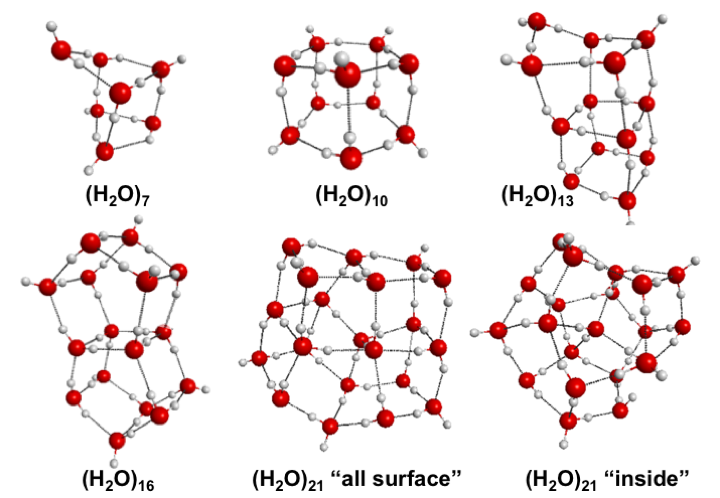
\includegraphics[width=\textwidth]{Figures/Chapter_2/cluster_structures.png}
\end{center}
\label{fig:MBE_I_F1}
\caption[Generating a facing caption page]{Water cluster isomers used in the MBE analysis.}
\end{figure}

\begin{figure}[t]
\uwsinglespace
\centering
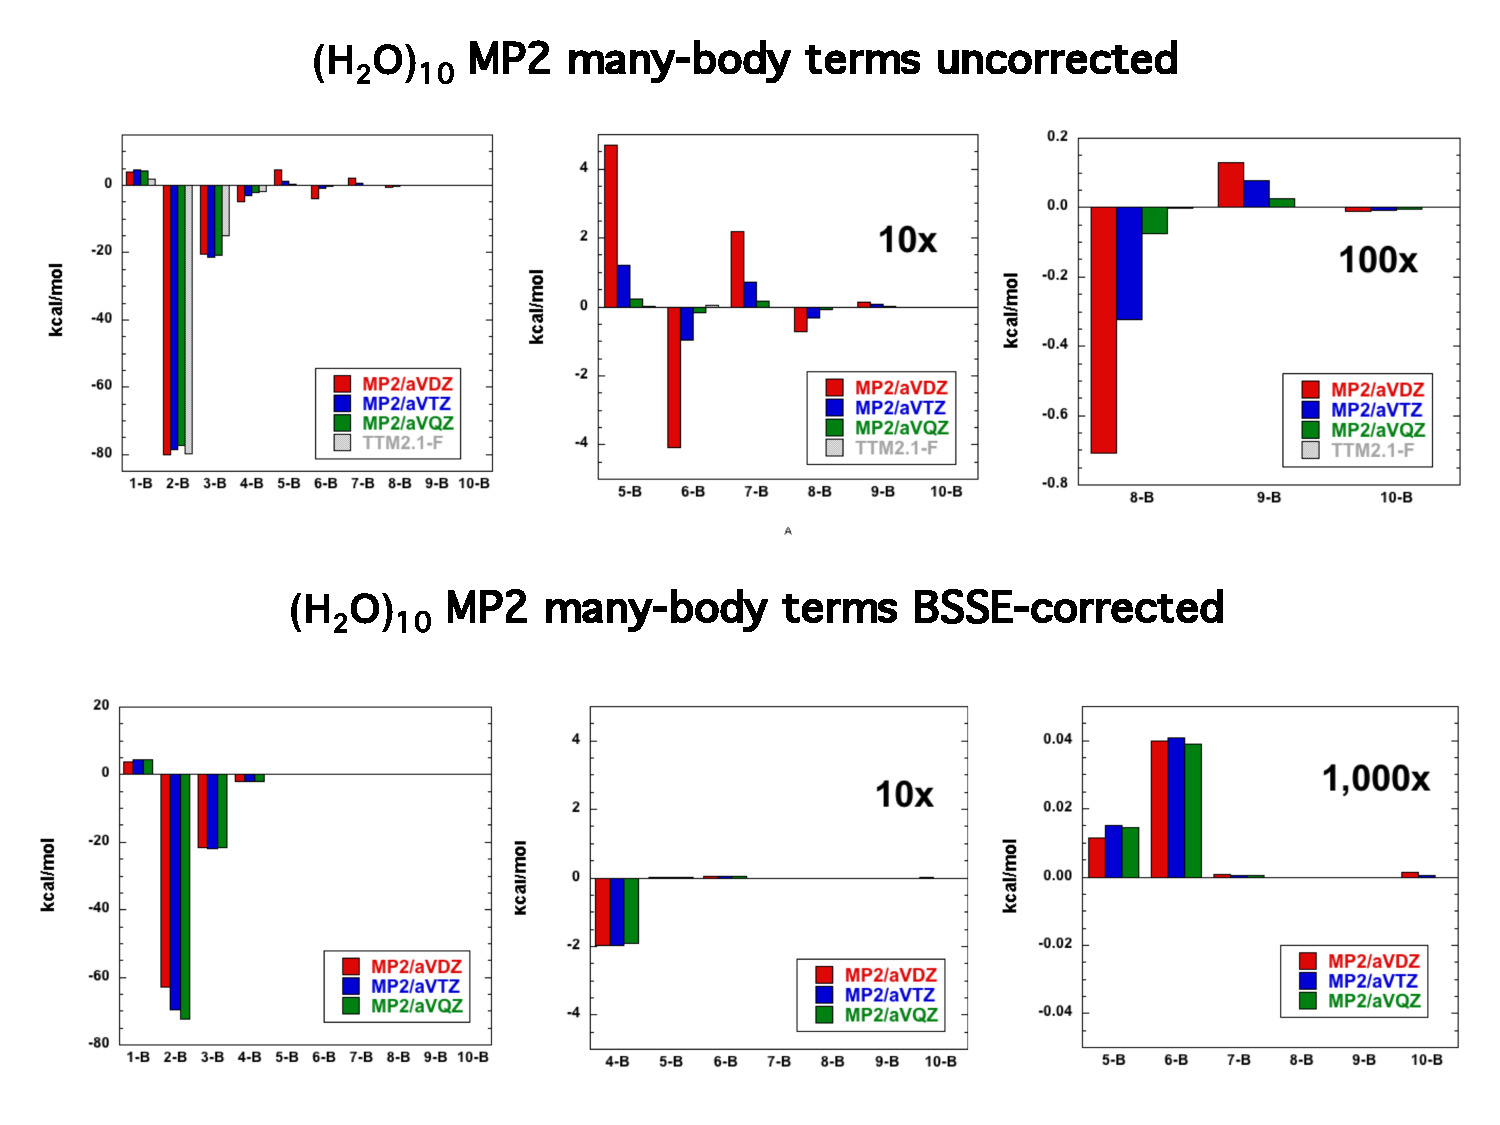
\includegraphics[width=\textwidth]{Figures/Chapter_2/W10_MP2_MB.pdf}
\label{fig:MBE_I_F2}
\caption[temp]{Magnitude of the uncorrected (top) and BSSE-corrected (bottom) 1- through 10-body MBE terms for the \ce{(H2O)_{10}} cluster. Note the magnification (10 – 1000X) of the y-axis in the middle and right panels used to indicate the small magnitude of the higher-order relative to the ones for the 2- and 3-body terms.}
\end{figure}

\begin{figure}[t]
\uwsinglespace
\begin{center}
\begin{minipage}{0.45\textwidth}
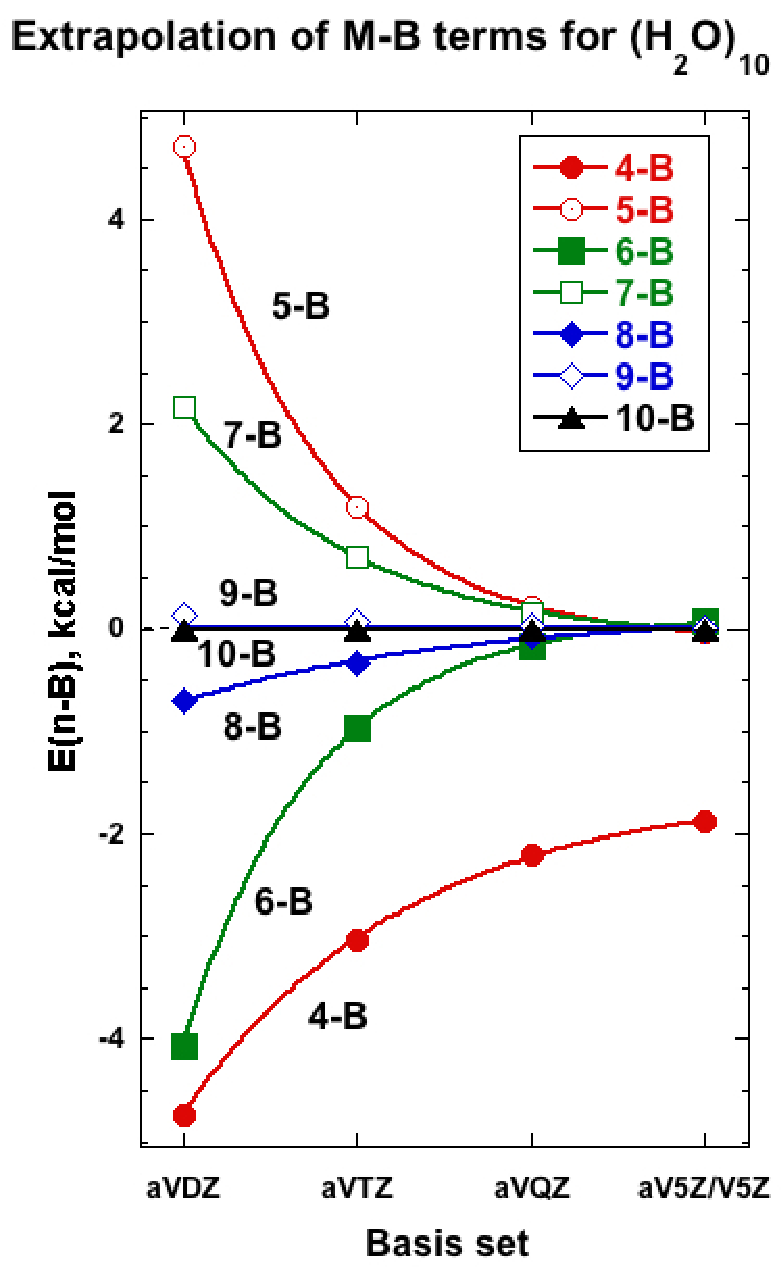
\includegraphics[width=.9\textwidth]{Figures/Chapter_2/MB_extrap_w10_noBSSE.pdf}
\end{minipage}
\begin{minipage}{0.45\textwidth}
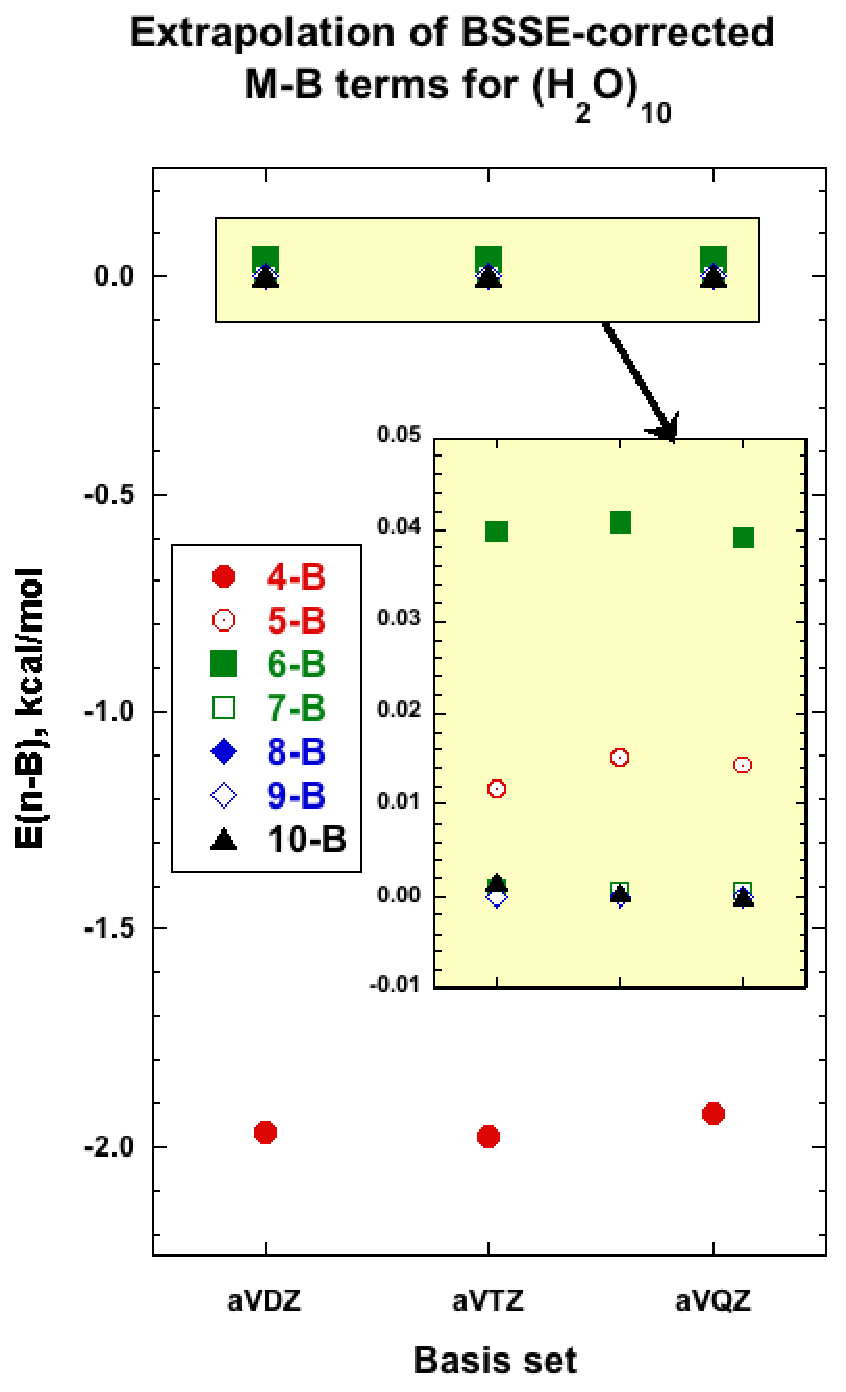
\includegraphics[width=.9\textwidth]{Figures/Chapter_2/MB_extrap_w10_BSSE_all.pdf}
\end{minipage}
\end{center}
\label{fig:MBE_I_F3}
\caption[temp]{Convergence of the uncorrected (left) and BSSE-corrected (right) 4- through 10-body terms in the many-body expansion for \ce{(H2O)_{10}} for the various basis sets. Notice the different y-axis scales.}
\end{figure}

\begin{figure}[t]
\uwsinglespace
\begin{center}
\begin{minipage}{0.45\textwidth}
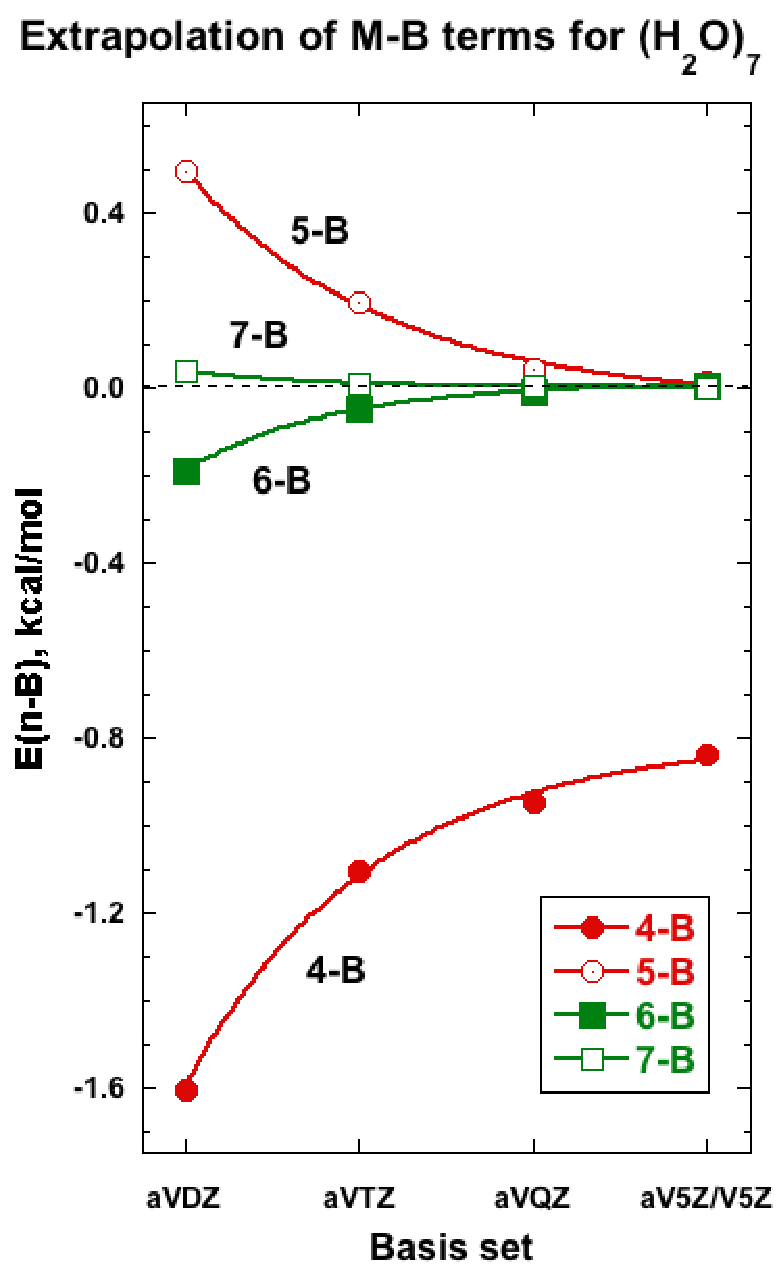
\includegraphics[width=.9\textwidth]{Figures/Chapter_2/MB_extrap_w7_noBSSE.pdf}
\end{minipage}
\begin{minipage}{0.45\textwidth}
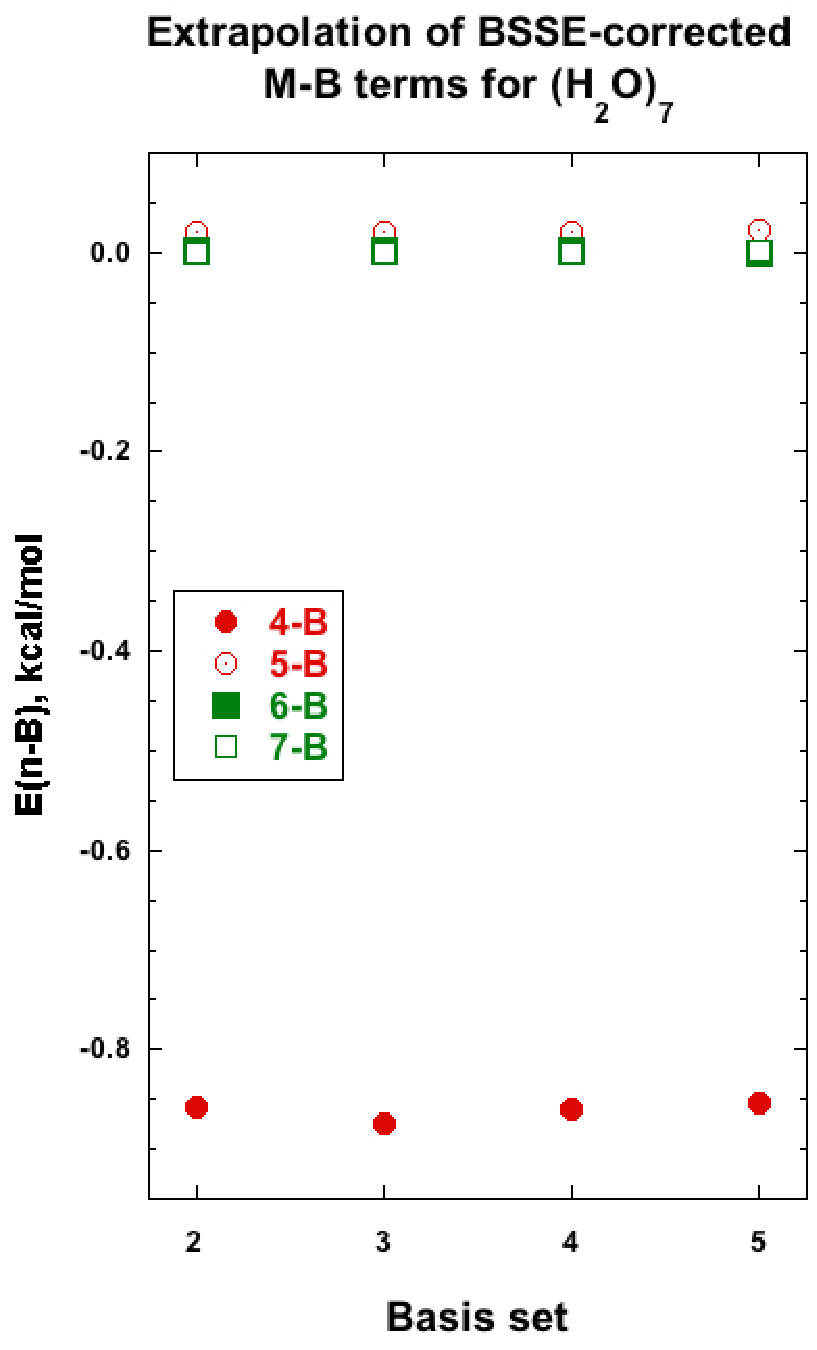
\includegraphics[width=.9\textwidth]{Figures/Chapter_2/MB_extrap_w7_BSSE.pdf}
\end{minipage}
\end{center}
\label{fig:MBE_I_F4}
\caption[temp]{Convergence of the uncorrected (left) and BSSE-corrected (right) 4- through 7-body terms in the many-body expansion for \ce{(H2O)7} for the various basis sets. Notice the different y-axis scales.}
\end{figure}

\begin{figure}[t]
\uwsinglespace
\begin{center}
\begin{minipage}{0.45\textwidth}
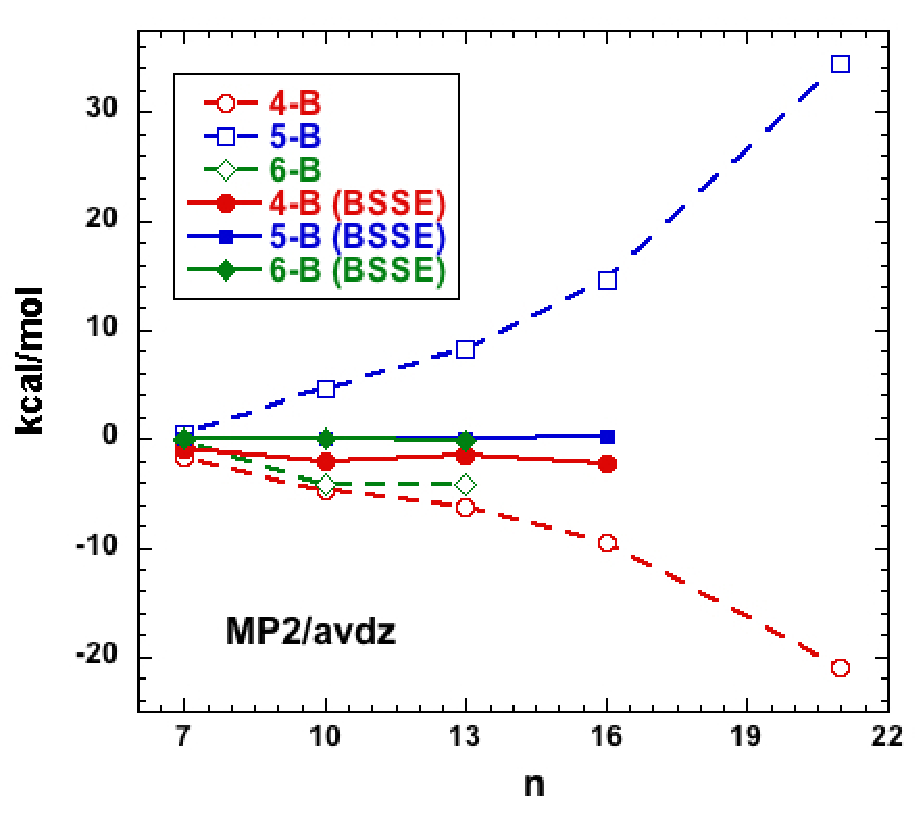
\includegraphics[width=.9\textwidth]{Figures/Chapter_2/4_B_6_B_vs_n.pdf}
\end{minipage}
\begin{minipage}{0.45\textwidth}
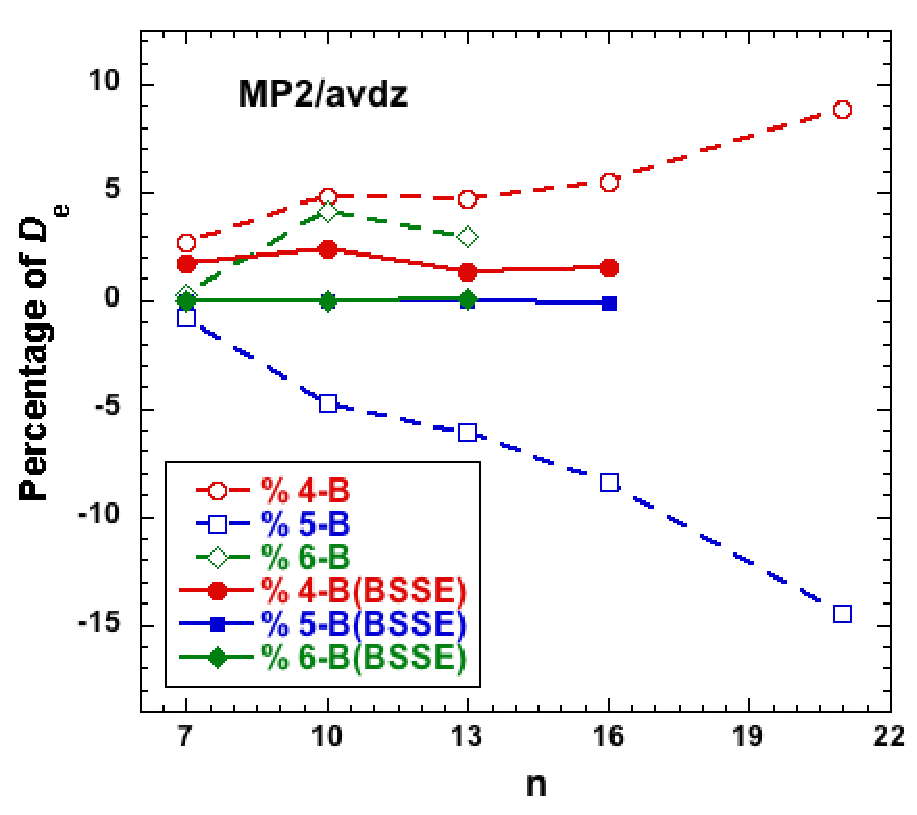
\includegraphics[width=.9\textwidth]{Figures/Chapter_2/4_B_6_B_perc_vs_n.pdf}
\end{minipage}
\end{center}
\label{fig:MBE_I_F5}
\caption[temp]{The absolute magnitudes (left) and percentage contributions (right) of the 4- to 6-body terms to the MP2/AVDZ binding energy for (H2O)n, n = 7, 10, 13, 16 and 21. The uncorrected (dashed lines) and BSSE-corrected results (solid lines) are shown.}
\end{figure}

\begin{figure}[t]
\uwsinglespace
\begin{center}
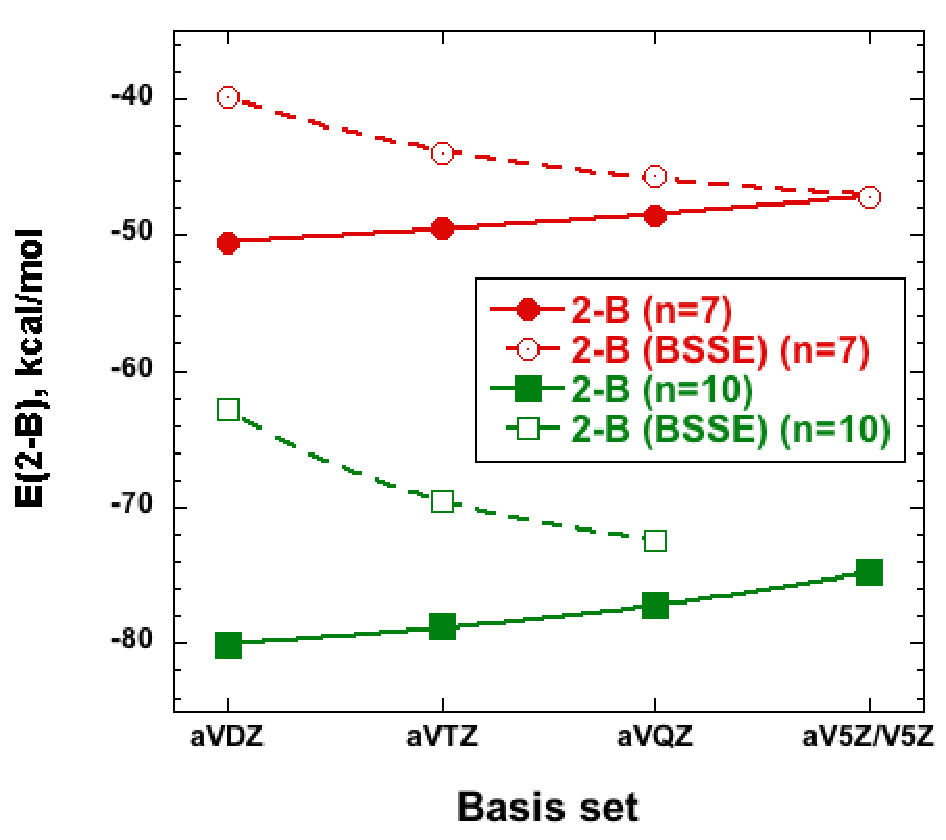
\includegraphics[width=\textwidth]{Figures/Chapter_2/E_2B_7_10.pdf}
\end{center}
\label{fig:MBE_I_F6}
\caption[temp]{Convergence of the uncorrected and BSSE-corrected total 2-body energy for \ce{(H2O)7} and \ce{(H2O)_{10}} with the AVXZ basis sets.}
\end{figure}

\begin{figure}[t]
\uwsinglespace
\begin{center}
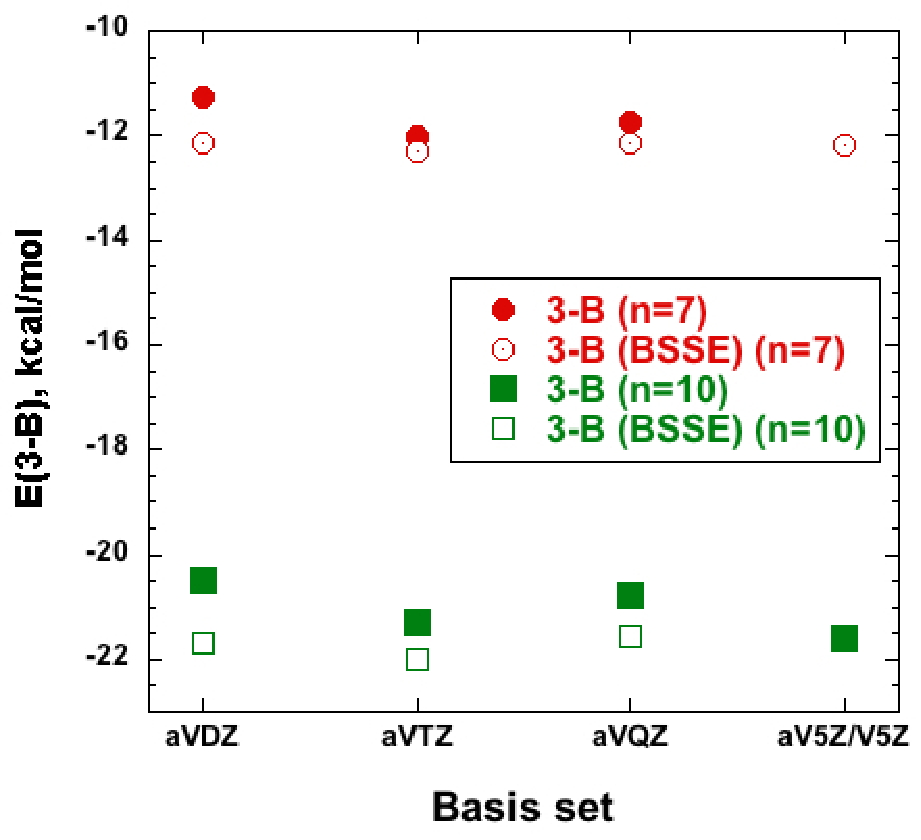
\includegraphics[width=\textwidth]{Figures/Chapter_2/E_3B_7_10.pdf}
\end{center}
\label{fig:MBE_I_F7}
\caption[temp]{Convergence of the uncorrected and BSSE-corrected total 3-body energy for \ce{(H2O)7} and \ce{(H2O)_{10}} with the AVXZ basis sets.}
\end{figure}

\begin{figure}[t]
\uwsinglespace
\begin{center}
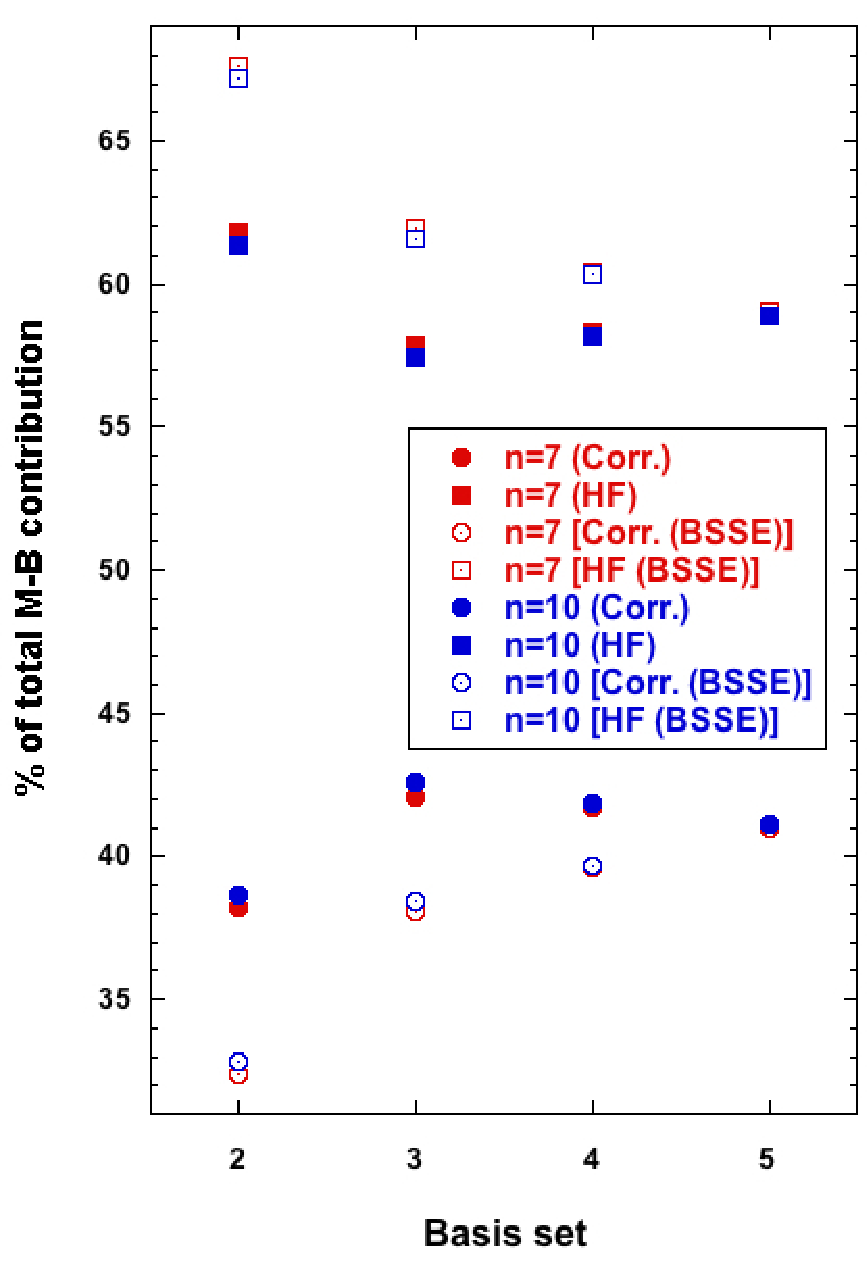
\includegraphics[width=\textwidth]{Figures/Chapter_2/percent_corr_HF_7_10.pdf}
\end{center}
\label{fig:MBE_I_F8}
\caption[temp]{Percentage of the total binding energy from HF and correlation for \ce{(H2O)7} and \ce{(H2O){10}} using the monomer and cluster basis at each of the AVXZ basis sets.}
\end{figure}

\begin{figure}[t]
\uwsinglespace
\begin{center}
\includegraphics[width=\textwidth]{Figures/Chapter_2/2body_bsse_decay_with_basis.pdf}
\end{center}
\label{fig:MBE_I_F9}
\caption[temp]{Variation of the BSSE correction for the 2-body terms with the O-O distance between fragments with the different basis sets used in this study. Solid lines represent least mean squares fits of the data to the function $a(1+erf(-bR_{OO}))$ for each basis set.}
\end{figure}

\begin{figure}[t]
\uwsinglespace
\begin{center}
\includegraphics[width=\textwidth]{Figures/Chapter_2/2body_bsse_correlation.pdf}
\end{center}
\label{fig:MBE_I_F10}
\caption[temp]{Predicted versus calculated BSSE correction for the individual 2-body terms of the clusters with the different basis sets used in this study.}
\end{figure}

\begin{table}[]
\centering
\begin{tabular}{@{}rrrrrrrrr@{}}
\toprule
     & \multicolumn{4}{c}{Uncorrected}         & \multicolumn{4}{c}{BSSE-corrected}      \\ \midrule
k    & AVDZ    & AVTZ    & AVQZ    & AV5Z/ V5Z & AVDZ    & AVTZ    & AVQZ    & AV5Z/ V5Z \\
\hline
\multicolumn{9}{c}{n = 7}                                                                \\
\hline
1-B  & 2.213   & 2.446   & 2.468   & 2.554     & 2.213   & 2.446   & 2.468   & 2.554     \\
2-B  & -50.578 & -49.459 & -48.626 & -47.160   & -39.894 & -43.958 & -45.712 & -47.165   \\
3-B  & -11.275 & -12.030 & -11.743 & -12.191   & -12.141 & -12.313 & -12.151 & -12.181   \\
4-B  & -1.606  & -1.106  & -0.950  & -0.841    & -0.858  & -0.874  & -0.861  & -0.854    \\
5-B  & 0.493   & 0.194   & 0.043   & 0.013     & 0.021   & 0.021   & 0.020   & 0.023     \\
6-B  & -0.192  & -0.051  & -0.010  & 0.003     & 0.002   & 0.001   & 0.001   & -0.0007   \\
7-B  & 0.037   & 0.008   & 0.002   & -0.0004   & 0.0001  & 0.0001  & 0.0001  & 0.0016    \\
\hline
\multicolumn{9}{c}{n = 10}                                                               \\
\hline
1-B  & 3.952   & 4.509   & 4.449   & 4.595     & 3.952   & 4.509   & 4.449   &           \\
2-B  & -80.165 & -78.707 & -77.249 & -74.796   & -62.762 & -69.504 & -72.387 &           \\
3-B  & -20.475 & -21.285 & -20.790 & -21.625   & -21.691 & -21.989 & -21.582 &           \\
4-B  & -4.742  & -3.028  & -2.202  & -1.878    & -1.968  & -1.978  & -1.923  &           \\
5-B  & 4.698   & 1.200   & 0.219   & -0.038    & 0.012   & 0.015   & 0.014   &           \\
6-B  & -4.081  & -0.964  & -0.179  & 0.071     & 0.040   & 0.041   & 0.039   &           \\
7-B  & 2.175   & 0.708   & 0.1594  & -0.008    & 0.001   & 0.0005  & 0.0005  &           \\
8-B  & -0.707  & -0.324  & -0.0758 & -0.003    & -0.0001 & -0.0001 & -0.0001 &           \\
9-B  & 0.131   & 0.078   & 0.0246  & 0.003     & 0.0000  & 0.0000  & 0.0000  &           \\
10-B & -0.010  & -0.008  & -0.0039 & -0.0006   & 0.0014  & 0.0004  & 0.0000  &           \\ \bottomrule
\end{tabular}
\caption{Magnitudes of the individual terms (kcal/mol) for the clusters \ce{(H2O)n}, n = 7, 10 with the various basis sets. Both the uncorrected and BSSE-corrected values are listed.}
\label{tab:MBE_I_T1}
\end{table}

\begin{table}[]
\centering
\begin{tabular}{@{}rrr@{}}
\toprule
k       & Uncorrected     & BSSE-corrected     \\ \midrule
\multicolumn{3}{c}{n =13}                      \\
\hline
1-B     & 4.527           & 4.527              \\
2-B     & -111.096        & -86.692            \\
3-B     & -26.264         & -28.335            \\
4-B     & -6.352          & -1.499             \\
5-B     & 8.243           & 0.056              \\
6-B     & -4.081          & -0.050             \\
\hline
\multicolumn{3}{c}{n =16}                      \\
\hline
1-B     & 6.456           & 6.456              \\
2-B     & -141.072        & -110.162           \\
3-B     & -35.514         & -37.944            \\
4-B     & -9.463          & -2.179             \\
5-B     & 14.560          & 0.181              \\
\hline
\multicolumn{3}{c}{n =21 					(“all-surface”)} \\
\hline
1-B     & 7.819           &                    \\
2-B     & -191.747        &                    \\
3-B     & -44.152         &                    \\
4-B     & -19.892         &                    \\
5-B     & 39.090          &                    \\
\hline
\multicolumn{3}{c}{n =21 (“inside”)}           \\
\hline
1-B     & 9.585           &                    \\
2-B     & -191.447        &                    \\
3-B     & -47.359         &                    \\
4-B     & -20.976         &                    \\
5-B     & 34.391          &                    \\ \bottomrule
\end{tabular}
\caption{Magnitudes of the individual terms (kcal/mol) for the clusters \ce{(H2O)n}, n = 13, 16, 21 at the MP2/AVDZ level of theory. Both the uncorrected and BSSE-corrected values are listed.}
\label{tab:MBE_I_T2}
\end{table}

\begin{table}[]
\centering
\begin{tabular}{@{}ccccc@{}}
\toprule
Cluster & 1-Body          & 2-Body           & Sum of 3- to 5-Body & Total Correlation \\ \midrule
\ce{(H2O)7}  & -3.73 (15.80)   & -19.77 (83.74)   & -0.105 (0.44)       & -23.609           \\
\ce{(H2O)_{10}} & -6.391 (16.59)  & -31.870 (82.75)  & -0.250 (0.65)       & -38.514           \\
\ce{(H2O)_{13}} & -9.135 (23.99)  & -29.0526 (76.31) & 0.135 (-0.35)       & -38.073           \\
\ce{(H2O)_{16}} & -12.051 (24.80) & -36.205 (74.49)  & -0.344 (0.71)       & -48.600           \\ \bottomrule
\end{tabular}
\caption{Contribution of the correlation energy to the various many-body terms for \ce{(H2O)n}, n = 7, 10, 13, 16. The results are obtained with the largest basis set used for each isomer (see text). The percentage of the total correlation energy is given in parentheses. Energies are in kcal/mol, while parentheses indicate the percentage of the total correlation energy.}
\label{tab:MBE_I_T3}
\end{table}

\begin{table}[]
\centering
\begin{tabular}{@{}lccc@{}}
\toprule
(H2O)3       & \multicolumn{1}{p{3cm}}{\centering MP2/AVQZ//\\MP2/AVQZ} & \multicolumn{1}{p{4cm}}{\centering CCSD(T)/AVQZ//\\MP2/AVQZ} & \multicolumn{1}{p{4cm}}{\centering CCSD(T)/AVQZ//\\CCSD(T)/AVQZ}\\
\hline
\textbf{Total Energy} & \textbf{-15.440}   & \textbf{-15.478}       & \textbf{-15.493}           \\
\hline
1-B          & 0.429              & 0.410                  & 0.346                      \\
2-B          & -13.359            & -13.428                & -13.479                    \\
3-B          & -2.510             & -2.460                 & -2.360           \\ \bottomrule         
\end{tabular}
\caption{The MP2/AVQZ and CCSD(T)/AVQZ 1-, 2-, and 3-body terms for \ce{(H2O)3} at the MP2/AVQZ and CCSD(T)/AVQZ geometries. The notation CCSD(T)/AVQZ//MP2/AVQZ means CCSD(T)/AVQZ energies are calculated the MP2/AVQZ optimized geometry. The relevant monomer reference energies (from left to right), in a.u., are -76.35191864, -76.36358738, and -76.3635876.}
\label{tab:MBE_I_T4}
\end{table}

\begin{table}[]
\centering
\begin{tabular}{@{}ccccc@{}}
\toprule
             & MP2/AVDZ          & CCSD(T)/AVDZ               & MP2/AVTZ          & CCSD(T)/AVTZ \\
             \hline
Total Energy & \textbf{-60.908 / -50.658} & \textbf{-60.841 / -49.900} & \textbf{-59.998 / -54.676} &              \\
\hline
1-B          & 2.213 / 2.213     & 2.075 / 2.075              & 2.446 / 2.446     & 2.372        \\
2-B          & -50.578 / -39.894 & -50.727 / -39.359          & -49.459 / -43.958 & -49.738      \\
3-B          & -11.275 / -12.141 & -10.811 / -11.710          & -12.030 / -12.313 & -11.636      \\
4-B          & -1.606 / -0.858   & -1.758 / -0.937            & -1.106 / -0.874   &              \\
5-B          & 0.493 / 0.021     & 0.553 / 0.027              & 0.194 / 0.021     &              \\
6-B          & -0.192 / 0.002    & -0.212 / 0.002             & -0.51 / 0.001     &              \\
7-B          & 0.037 / 0.000     & 0.040 / 0.000              & 0.008 / 0.000     &             \\ \bottomrule
\end{tabular}
\caption{The MP2/AVXZ and CCSD(T)/AVXZ BSSE-uncorrected and BSSE-corrected interaction energies for \ce{(H2O)7} in the format $E_{uncorr}$ / $E_{corr}$ all carried out at the MP2/AVXZ geometry for X=D, T. The relevant water monomer reference energies (from left to right), in a.u., are -76.26090977, -76.27390289, -76.3289924, and -76.34232562. We do not report the BSSE-corrected numbers for CCSD(T)/AVTZ due to the computational expense.}
\label{tab:MBE_I_T5}
\end{table}

\begin{table}[]
\centering
\begin{tabular}{@{}ccccc@{}}
\toprule
\textbf{Basis set}  & \textbf{a} & \textbf{b} & $\mathbf{\chi}$ & \textbf{R} \\
\hline
aug-cc-pVDZ         & 14.435 & 0.4639 & 0.1342 & 0.9946 \\
aug-cc-pVTZ         & 9.445  & 0.4887 & 0.0386 & 0.9948 \\
aug-cc-pVQZ         & 5.549  & 0.4998 & 0.0131 & 0.9937 \\
aug-cc-pV5Z/cc-pV5Z & 11.211 & 0.6728 & 0.0006 & 0.9931 \\ \bottomrule
\end{tabular}
\caption{Fit of the 2-body BSSE correction via eq. \eqref{eq:MBE_I_2} for the various basis sets.}
\label{tab:MBE_I_T6}
\end{table}

\chapter{The many-body expansion for aqueous systems revisited: II. Alkali metal and halide ion-water interactions}

\section{Introduction}
\par The Many-Body Expansion (MBE) underpins a number of recent many-body, non-additive classical potential energy surfaces, especially those involving water\autocite{burnham_development_2002,fanourgakis_flexible_2006,fanourgakis_development_2008,heindel_benchmark_2018,wang_flexible_2011,babin_development_2013,das_development_2019,gora_predictions_2014} that are fitted to ab-initio data for clusters. While the concept of the MBE has resulted in some of the most accurate classical interaction potentials created to date, these potentials only exist for a relatively narrow range of systems for which they were parametrized. Most notably, there is an ever-present interest in understanding the details of molecular interactions between water and various solutes, such as ions. There is also interest in elucidating the effects of these ions, especially in higher concentrations, in modifying the interactions among neighboring water molecules and how this alters the resulting dynamics of these systems. Additionally, the interactions between water and ions are paramount in understanding the physical mechanisms behind many chemical and biological processes such as aqueous solvation\autocite{makarov_solvation_2002,collins_ions_2004}, ion channels\autocite{pinto_influenza_1992,shearman_modulation_1989} and electrochemistry.\autocite{zhang_effects_2011,liu_doping_2006,tang_dynamic_2011}

\par Ions have been known to alter the local hydrogen bonding network in water by inducing local disruptions depending on their charge state.\autocite{marcus_ions_2015,chang_recent_2006,hribar_how_2002} Positively charged ions attract neighboring water molecules as acceptors (A) via their oxygen atoms, whereas negatively charged ones as donors (D) via their hydrogens. The distinct local arrangement of the nearest-to-ion-neighbor water molecules (i.e., the first solvation shell) induces a local structure in subsequent solvation shells away from the ion. For example, in the case of positively charged ions the first solvation shell water molecules participate in hydrogen bonds with molecules in the second solvation shell exclusively as (D), whereas for negatively charged ions as both (D) and (A). Nevertheless, the effect of the ions in altering the interaction between neighboring water molecules in clusters has been quantified by both experimental infrared and computational ab-initio studies. The former record the changes of the red shifts in the OH stretching vibrational bands that occur due to the strengthening/weakening of the hydrogen bonds,\autocite{horvath_anharmonicities_2010,bush_infrared_2008,duncan_spectroscopy_1997,ayotte_spectroscopic_1999,dorsett_probing_1999} while the latter provide quantitative information about the change in the two-body water-water interaction due to the presence of a nearby ion.\autocite{xantheas_theoretical_1995,xantheas_quantitative_1996}

\par Ions are also known to affect the structure and overall stability of solutes in aqueous environments. For example, the extent to which an ion affects processes involving a protein, which was first realized in 1888,\autocite{hofmeister_zur_1888} is described by the Hofmeister series. In other cases, the ion identity greatly affects the rates and even outcomes of certain biological processes,\autocite{zhang_interactions_2006} with the molecular level mechanism responsible for these changes still not fully understood. The view that the ions affect processes in aqueous environments by disrupting the hydrogen-bonding network of water\autocite{marcus_effect_2009} has resulted into their categorization to “structure-makers” or “structure-breakers”.\autocite{collins_hofmeister_1985} The notion that ions can have long-range effects on the hydrogen-bonding network of liquid water is supported by previous spectroscopic\autocite{omta_influence_2003,omta_negligible_2003,kropman_vibrational_2003,kropman_effect_2004} and thermodynamic\autocite{batchelor_impact_2004} studies with some recent studies even suggesting than a single ion has an influence on millions of surrounding water molecules.\autocite{chen_electrolytes_2016} Spectroscopic 2-D infrared measurements in the region of the OD stretch in HDO molecules in the presence of various ions aim at measuring the orientational correlation time of water outside the first solvation shell of the ions. More recent 2-D Raman-THz measurements, which directly probe the intermolecular hydrogen-bond stretching region, provide support for the structure-making and structure-breaking scenarios by correlating the relaxation time of the stretch to the B-coefficient36 of the cation in solution.\autocite{shalit_terahertz_2017} The authors conclude that this correlation “confirms the empirically used concept of structure makers or structure breakers on a molecular level.”\autocite{shalit_terahertz_2017} However, some disagreement over whether or not, and to what extent, various ions affect the long range hydrogen-bonding network of bulk aqueous ionic solutions still remains. Attempting to perform and interpret experiments in regions far away from the ion, especially in concentrated ionic solutions remains a fundamental challenge.

\par Experimental relaxation times from 2-D Raman-THz measurements suggested a rather strong correlation to the properties of the cation while being insensitive to the anion; for instance, \ce{SrCl2} vs. \ce{SrBr2} has no measurable effect on the relaxation time.\autocite{shalit_terahertz_2017} This is in direct contrast to the conventional wisdom that the anion produces the larger Hofmeister effect due to the dominating role of ionic dispersion at larger ionic concentrations and near interfaces.\autocite{bostrom_why_2004,jungwirth_molecular_2001,jungwirth_ions_2002,dang_molecular_2002,garrett_ions_2004} Therefore, it has been rationalized that anions should be the more important species due to their greater polarizabilities relative to the cations.\autocite{yang_hofmeister_2009} On the other hand, one might expect a cation to have a much greater effect on the surrounding hydrogen-bonding network of water due to the fact that cations must be stabilized via the oxygen atom, rather than donation of electron density via the hydrogen atom as in normal hydrogen bonds.\autocite{kwan_effect_2019} We will discuss ramifications of this effect in more detail later, when we present an anomaly arising in the presence of a cation but not an anion.

\par The previous discussion suggests that ion specificity plays a crucial role in determining the properties of aqueous ionic systems. To this end, the accurate description of the underlying interactions plays a crucial role in rendering a molecular level picture of the origin of these effects. The field of developing classical potentials for ion-water interactions has been active for the last 30 years\autocite{probst_molecular_1985,limtrakul_solvent_1985,probst_study_1987,amira_molecular_2004,wick_computational_2009,wick_molecular_2008} with efforts continuing up to this day.\autocite{arismendi-arrieta_i-ttm_2015,bajaj_toward_2016,riera_i-ttm_2016} Advances in computer hardware and software have also allowed for electronic structure driven molecular dynamics\autocite{car_unified_1985,kuhne_second_2014} simulations of aqueous ionic solutions,\autocite{todorova_carparrinello_2008,bako_carparrinello_2002,bankura_hydration_2013,baer_local_2016,duignan_quantifying_2020} so that a separate parameterization is not required for each ion but rather depends upon the level of electronic structure theory used. Nevertheless, the ensuing dynamics need to be propagated via the many-body terms in order to reduce the computational cost associated with these simulations while still allowing the use of a high level of theory.\autocite{liu_hydrogen-bond_2018,liu_variational_2019} 

\par In a previous paper\autocite{heindel_many-body_2020} (hereafter referred to as paper MBE-I) we have investigated the convergence of the many-body terms for water clusters with the level of electron correlation and basis set. We found that 5-body and higher terms converge monotonically to zero upon increasing the basis set towards the Complete Basis Set (CBS) limit and this behavior is accurately reproduced even with the smaller (aug-cc-pVDZ) set when the Basis Set Superposition Error (BSSE) is taken into account. In addition, it was found that neglecting the correlation contribution in all terms above the 3-body resulted in an error of the order of 0.1\%. Most importantly, the BSSE correction for the largest 2-body term in the MBE followed very closely the relation $a(1+erf(-bR))$, where $R$ is the distance between the two (either nearest or distant) oxygen atoms of the corresponding dimer. In the present paper we build upon these previous findings by extending the study of the MBE terms for ion-water clusters. We present detailed calculations focusing on the many-body terms of ionic clusters incorporating either a positive or negative ion on both the inside and outside of the cluster with a specific emphasis of how the guest ion changes the water-water interaction in the host’s hydrogen bonding network. The paper is organized as follows. In Section \ref{sec:MBE_2_sec_2} we describe our approach and outline the computational details used in this study. In Section \ref{sec:MBE_2_sec_3} we present the variation of the many-body terms with basis set as well as the BSSE corrections and their fitting to a universal function. Final conclusions are drawn in Section \ref{sec:MBE_2_sec_4}.

\subsection{Approach and Computational Details} \label{sec:MBE_2_sec_2}
\par We have extensively described the methods by which we perform the MBE in the preceding publication of this series\autocite{heindel_many-body_2020} as well as in earlier publications,\autocite{xantheas_ab_1994,xantheas_cooperativity_2000} so we will only briefly review the pertinent details here. The MBE is a means of decomposing some molecular property into contributions from various fragments of the total system. In the case of the total interaction energy, $D_e$, which is our focus in this work, the MBE can be cast as,\autocite{xantheas_ab_1994,xantheas_cooperativity_2000,hankins_water_1970}
$$
D_e=\sum_{i=1}^nE_{iB}=E(1,2,...,n)-\sum_{i=1}^nE_{ref,i}
$$
where $E_{ref,i}$ is the reference energy of the isolated fragment $i$. Furthermore, each of the $i$-body terms, $E_{iB}$, can be written as,
$$
E_{1B}=\sum_{i=1}^n[E(i)-E_{ref,i}]
$$
$$
E_{2B}=\sum_{i<j}[E(i,j)-E(i)-E(j)]
$$
$$
E_{3B}=\sum_{i<j<k}[E(i,j,k)-E(i,j)-E(i,k)-E(j,k)+E(i)+E(j)+E(k)]
$$

and so on for the $4$- through $n$-body terms. In the above notation, the term $E(i,j,k)$ corresponds to the energy of a trimer containing fragments $i$, $j$, and $k$.

\par The various energy terms are computed at some level of electronic structure theory with an atom-centered basis set, which is usually far from being complete. This introduces the additional complication of the Basis Set Superposition Error (BSSE), i.e. the compensation of each fragment’s basis set incompleteness by using functions from the basis set of its neighbors. The error due to this effect is estimated by computing all energies in the presence of the basis functions of the full system.\autocite{richard_understanding_2018,boys_calculation_1970,xantheas_importance_1996}

\par In this work we compute the MBE terms for aqueous clusters of alkali metal \ce{M} = \ce{Li^+}, \ce{K^+}, \ce{Cs+} and halide \ce{X} = \ce{Cl^-}, \ce{Br^-}, and \ce{I^-} clusters. We chose the cluster size of 10 fragments, \ce{Z^{+/-}(H2O)9}, in order to directly compare the results with the ones previously reported for a water cluster of the same number of “bodies”, \ce{(H2O)_{10}}. Our previous study (paper MBE-I) indicated that this cluster is large enough that certain artifacts attributed to BSSE are more evident and in addition we can meaningfully distinguish between the “ion-inside” and “ion-outside” isomers of the cluster. The two topologically different isomers correspond to the two cases when the ion resides on the surface or the inside of the water cluster. These geometries were selected by running NVT molecular dynamics trajectories with the Dang-Chang potential\autocite{dang_molecular_1997} and choosing frames in which the ion was clearly on the inside or outside of the structure and then optimizing these structures at the MP2/aug-cc-pVXZ level of theory (X = D, T, Q, 5). We will hereafter refer to Dunning’s augmented correlation consistent basis sets\autocite{dunning_gaussian_1989,wilson_gaussian_1999,woon_gaussian_1993} as aVXZ (X = D, T, Q, 5). In the case of \ce{Cl^-(H2O)9}, \ce{Br^-(H2O)9}, and \ce{I^-(H2O)9} we did not find any frames in which the chloride clearly resided on the inside of the cluster. Therefore, we constructed a constrained structure in which the halide ion is tetrahedrally coordinated by four water molecules, and the remaining five water molecules are attached to this first solvation shell. All degrees of freedom were then allowed to relax during the optimization subject to the condition that the chloride remains tetrahedrally coordinated. For the two isomers of the \ce{Li^+(H2O)9} and \ce{Cl^-(H2O)9} clusters the MBE was carried out to full rank (k = 10) with the basis aVDZ, aVTZ, aVQZ, and aV5Z for \ce{Cl}, \ce{O} and V5Z for \ce{H} for \ce{Cl^-(H2O)9} (hereafter denoted as aV5Z/V5Z) in order to investigate whether the variation of the terms with $k >= 5$ (without and with BSSE corrections) with basis set resembles the oscillatory behavior observed for \ce{(H2O)_{10}}. Since for \ce{Li^+(H2O)9} and \ce{Cl^-(H2O)9} it was indeed confirmed (\textit{vide infra}) that the BSSE corrected MP2/aVDZ results for $k >= 5$ resemble the MP2/CBS values, for the rest of the cations (\ce{K^+}, \ce{Cs^+}) and anions (\ce{Br^-}, \ce{I^-}) the MBE analysis was performed with just the aVDZ basis set with and without BSSE corrections. For calculations involving \ce{Cs^+} we used the Stuttgart pseudo-potential,\autocite{leininger_accuracy_1996} while for calculations involving \ce{I^-}, we used a pseudo-potential suggested by Peterson.\autocite{peterson_systematically_2003}

\subsection{Results and Discussion} \label{sec:MBE_2_sec_3}
\subsubsection{Many-Body terms of \ce{Li^+(H2O)9}, \ce{Cl^-(H2O)9} and their variation with basis set} \label{sec:MBE_2_sec_3a}

\par We first examine the variation of the MBE terms for the \ce{Li^+(H2O)9} and \ce{Cl^-(H2O)9} clusters. In particular, we focus on analyzing the total 2-, 3- and 4-B interactions (k = 2 – 4) and further on investigating the variation of the $k >= 5$ terms with basis set. For these higher order terms the question is whether there also exists an undulation between positive and negative values with effective convergence to zero for a large (aV5Z) basis set for the uncorrected numbers and effective convergence to CBS even with the aVDZ basis set for the $k >= 5$ terms upon inclusion of BSSE corrections, as previously observed in paper MBE-I for the pure water clusters. We will first discuss the results for the various isomers of those 2 clusters before moving on to the rest of the ionic clusters considered in this paper.

\textbf{2-B interaction (k = 2):} The variation of the total 2-B energy with basis set is shown in Figure \ref{fig:MBE_II_2} for the two isomers of the \ce{Li^+(H2O)9} and \ce{Cl^-(H2O)9} clusters. Due to the largest ion-water interaction, the total 2-B energy for \ce{Li^+(H2O)9} is larger than for the \ce{Cl^-(H2O)9} cluster. A qualitative difference is also observed between the two ionic systems, in that the total 2-B energy for ion inside isomer for \ce{Li^+(H2O)9} is larger compared to the ion outside isomer of that cluster while this trend is reversed for \ce{Cl^-(H2O)9}. We will attempt to explain these differences by partitioning the total 2-B interaction to its individual components, namely the ion-water (I-W) and water-water (W-W) 2-B interactions. Figure \ref{fig:MBE_II_3} shows the variation of the individual (I-W) and (W-W) 2-B terms (both uncorrected and BSSE corrected) with basis set for the ion inside and ion outside isomers of \ce{Li^+(H2O)9} (left panel) and \ce{Cl^-(H2O)9} (right panel) clusters. Note that the same y-axis scale is used in the two plots in order to make the comparison more direct. The individual and total 2-B terms exhibit the usual variation of the uncorrected and BSSE-corrected numbers with basis set towards a CBS limit. In all cases, the BSSE-corrected total interaction energy is less than the uncorrected one in accordance with the fact that this holds for each individual term in the sum. The individual (I-W) charge-dipole interactions are much stronger than the (W-W) dipole-dipole interactions and, despite the fact there are 9 of the former and 36 of the latter, their sums yield a total (I-W) 2-B interaction that is much larger than the total (W-W) 2-B interaction. As regards the trends related to the placement of the ion within the water cluster network, in general the ion inside geometry results in more ion-water bonds (ion surrounded by water molecules) that disrupt and weaken the water network. This is reflected by the relative strengths of the total (W-W) and (I-W) interactions for the ion inside and ion outside configurations shown in Figure \ref{fig:MBE_II_3}: the total (W-W)/(I-W) 2-B term for the ion inside geometry is less/more than the one for the ion outside geometry; in other words the ion inside configuration has stronger (I-W) and weaker (W-W) total 2-B interactions as it makes more ion-water bonds and induces a larger disruption of the water hydrogen bonding network than the ion outside configuration.

\par The difference in the magnitude of the (W-W) terms for each of the two ionic systems (< 10 kcal/mol for both the ion inside and ion outside isomers) is indicative of the large effect which a cation has on disrupting hydrogen-bonding interactions amongst water molecules. This is because incorporating a cation into a hydrogen-bonding network requires a water molecule to interact via the oxygen as opposed to the hydrogen atom for the case of an anion. This is one of the reasons that the hydrogen bond lifetime depends more strongly on the cation identity while being almost indifferent of the identity of the anion, as was previously experimentally observed.\autocite{shalit_terahertz_2017}

\par In summary, the fact that the total 2-B interaction for \ce{Li^+(H2O)9} is larger than the one for \ce{Cl^-(H2O)9} has its origins in the stronger (I-W) interaction of the former compared to the latter. In addition, the relative ordering of the total 2-B interaction between the ion inside vs. ion outside configurations is mainly driven by the (I-W) interaction as the ordering of the (I-W) interaction is the same with the total 2-B for the two different arrangements. The stronger (I-W) interaction (\ce{Li^+}$...$\ce{H2O} compared to \ce{Cl^-}$...$\ce{H2O}) was found to correlate with a stronger (W-W) interaction as well.

\textbf{3-B interaction (k = 3):} The variation of the total 3-B interaction with basis set is shown in Figure \ref{fig:MBE_II_4} for the two isomers of the \ce{Li^+(H2O)9} and \ce{Cl^-(H2O)9} clusters. The total 3-B terms are repulsive (destabilizing) for both ionic clusters and structural arrangements (Figure \ref{fig:MBE_II_4}). Note that for the 3-B term the BSSE correction does not always result in numbers that are lower than the uncorrected ones. The spread of the total 3-B energies for the two isomers of \ce{Li^+(H2O)9} (upper panel of Figure \ref{fig:MBE_II_4}) is much larger than the one found for the two isomers of the \ce{Cl^-(H2O)9} cluster (lower panel of Figure \ref{fig:MBE_II_4}); as in the case for the total 2-B interaction, the order of the total 3-B energies for the two structural arrangements is reversed between the two ionic clusters (more repulsive for the ion inside isomer of \ce{Li^+(H2O)9}, less repulsive for the same isomer of \ce{Cl^-(H2O)9}). Although the 3-B energies are in the 0-6 kcal/mol range for both isomers of \ce{Cl^-(H2O)9} and the ion outside isomer of \ce{Li^+(H2O)9}, we note a much larger (\textapprox20 kcal/mol) repulsive total 3-B energy for the ion inside isomer of the latter. This may suggest that both the strength and the total number of the (I-W) interactions influence the total 3-B energy. In Figure \ref{fig:MBE_II_5} we attempt to partition the total 3-B energies in terms of the individual (I-W-W) and (W-W-W) contributions for each ionic cluster. In the following we will assign the 3-B interactions as strong/weak based on a negative scale, i.e., a larger repulsive (destabilizing) interaction is described as “weaker” than a smaller repulsive (stabilizing) one, which is described as “stronger”. The two panels of Figure \ref{fig:MBE_II_5} are plotted with the same y-axis scale to make the comparison easier. For the ion inside isomer of the \ce{Li^+(H2O)9} cluster there exists a large (\textapprox25 kcal/mol) repulsive (I-W-W) interaction that is partially offset by a much smaller (\textapprox6 kcal/mol) attractive (W-W-W) interaction. Both of these interactions are smaller (\textapprox5 and \textapprox1 kcal/mol) and repulsive for the ion outside isomer of that cluster. In contrast, in the ion inside isomer of the \ce{Cl^-(H2O)9} cluster both components are quite small (\textless 2 kcal/mol) and repulsive, whereas for the ion outside isomer of this cluster they have opposite signs (the (W-W-W) interaction is attractive) and almost cancel each other. 

\par From the limited sampling of configurational space examined here (i.e., just two conformations with the ion inside and outside a water network) we are not able to arrive at general conclusions regarding the sign and magnitude of the 3-B (I-W-W) and (W-W-W) terms based on either the strength or the number (coordination) of the (I-W) interactions. Indeed, when comparing \ce{Li^+} vs. \ce{Cl^-}, a stronger (I-W) interaction (Li+) is associated with a weaker (I-W-W) and a stronger (W-W-W) interaction for the ion inside isomer, but the situation is reversed for the ion outside isomer which has a stronger (I-W-W) and a weaker (W-W-W) interaction. This is also easily seen by the relative positions of the red (ion inside isomer) and green lines (ion outside isomer) in the two panels of Figure \ref{fig:MBE_II_5}: the green lines lie in between the red ones in the left panel, while the situation is reversed (red lines in between the green ones) in the right panel. That is, for the inside isomers, where the number of (I-W) bonds is larger, \ce{Li^+} results in weaker (I-W-W) and stronger (W-W-W) interactions, whereas the situation is reversed for \ce{Cl^-}.

\par It is worth noting that the two most repulsive total (I-W-W) terms for the ion inside isomer of \ce{Li^+(H2O)9} (left panel of Figure \ref{fig:MBE_II_5}) and ion outside isomer of \ce{Cl^-(H2O)9} (right panel of Figure \ref{fig:MBE_II_5}) correspond to the cases associated with the most stabilizing total (W-W-W) interactions. While we cannot make definitive generalizations from the limited sampling of configurations studied here, this may indicate a type of anti-cooperative effect between the ion-water interactions and the water-only hydrogen bonding networks. This follows from the fact that the 3-body term is a sensitive measure of the degree of cooperativity in aqueous clusters.\autocite{xantheas_cooperativity_2000} The fact that the ion-water interactions weaken the ability of water to hydrogen-bond cooperatively\autocite{xantheas_cooperativity_2000} is also evident from the fact that the (W-W-W) terms are barely stabilizing or essentially zero for both cases. These terms are much smaller in magnitude and as a percentage of the total binding energy (vide infra) than the corresponding ones previously found for pure water clusters.\autocite{heindel_many-body_2020}

\par Another interesting point is that the (I-W-W) interactions are destabilizing by about 25 kcal/mol when \ce{Li^+} resides on the inside of the water cluster. On the other hand, the (I-W) interactions are more strongly stabilizing for the inside isomer of \ce{Li^+(H2O)9}. These observations reinforce the idea that cations tend to disrupt the hydrogen-bonding network in water so that water has a difficult time favorably interacting with itself. Therefore, the relatively large role of many-body terms for a cation compared to an anion is perhaps counter-intuitive when we tend to associate many-body effects with induction and polarizability,\autocite{heindel_origin_2018,zhuang_many-body_2019} which one would also expect to be larger in anionic systems.

\par In terms of the trends observed in Figure \ref{fig:MBE_II_4}, the magnitude of the total 3-B term is mainly determined by the (I-W-W) interaction. This interaction is substantial for the ion inside arrangement of the \ce{Li^+(H2O)9} cluster but quite small for its outside arrangement as well as for both arrangements of the \ce{Cl^-(H2O)9} cluster. The above findings justify the previous use of an (I-W-W) 3-B exchange potential for the modeling of the solvation of strongly bound ions (\ce{Li^+} and \ce{F^-}) in water, i.e. arrangements that the ion is fully solvated,\autocite{dang_ion_1991,xantheas_critical_1996} whereas the inclusion of this additional interaction did not seem to make a difference for the solvation of \ce{Cl^-} ions in water.\autocite{perera_structures_1994}

\textbf{4-B interaction (k = 4):} The importance of M-B terms beyond the 3-B for aqueous systems was somewhat unclear for a while, but recently a consensus has been reached that including the 4-body term is quite important if one is interested in accuracies on the order of 1 kcal/mol.\autocite{heindel_benchmark_2018,lao_understanding_2016,richard_aiming_2014,howard_n-body_2013} This raises the question whether the MBE actually converges smoothly, or if terms beyond the 4-B are also necessary. In our first paper of this series,\autocite{heindel_many-body_2020} we have conclusively shown that terms beyond the 4-body are practically negligible in calculations of the binding energy of neutral water clusters, which agrees with similar calculations done previously at the Hartree-Fock level.\autocite{ouyang_trouble_2014,ouyang_many-body_2015} This statement comes with the caveat that one includes a proper correction for BSSE, which will otherwise cause the 5-body and higher-order terms to erroneously appear to be large and oscillating in magnitude around zero.

\par Figure \ref{fig:MBE_II_6} shows the variation of the total 4-B interaction with basis set for the two isomers of the \ce{Li+(H2O)9} and \ce{Cl-(H2O)9} clusters. The interaction is practically zero except for the ion inside isomer of the \ce{Li^+(H2O)9} cluster, for which the main contribution (\textgreater 95\% at the aVQZ, BSSE corrected) comes from the (I-W-W-W) interaction. These results suggest that the 4-B term can be safely omitted when modeling the various arrangements of the ion in the Cl-(H2O)9 cluster and structures in which the \ce{Li^+} ion resides on the surface of a water cluster; however, this will result in an error of \textapprox5\% for configurations where the \ce{Li^+} ion is fully solvated by a water network.

\textbf{Higher order interactions (k = 5 – 10):} The variation of the 4- through 10-body terms with basis set for the ion outside and ion inside isomers is shown in Figure \ref{fig:MBE_II_7} for the \ce{Li^+(H2O)9} and Figure \ref{fig:MBE_II_8} for the \ce{Cl^-(H2O)9} clusters, respectively. In each Figure there are 4 panels, two for the ion outside (top) and two for the ion inside (bottom). The left panels (top, bottom) trace the uncorrected, while the right panels (top, bottom) the BSSE corrected numbers.

\par In general, we observe a pattern in the variation of the higher order ($k >= 5$) MBE terms with basis set that is similar to the one observed earlier for pure water clusters,\autocite{heindel_many-body_2020} namely an undulation around zero for the even and odd MBE terms and their convergence to practically zero with the larger basis set used in this study (aV5Z/V5Z). All BSSE-corrected MB terms ($k >= 4$) are practically constant with basis set size, a result similar to the one previously found for pure water clusters.\autocite{heindel_many-body_2020} However, the convergence of the BSSE-uncorrected 4-B term is in some instances not monotonic with basis set. For example, the BSSE uncorrected 4-B term for the outside isomers of both ions (top left panels in Figures \ref{fig:MBE_II_7} and \ref{fig:MBE_II_8}) switches from a small negative to a small positive value going from the aVQZ to the aV5Z/V5Z basis set. This change in sign is real as confirmed from the positive BSSE-corrected values of the 4-B term for these isomers (top right panels in Figures \ref{fig:MBE_II_7} and \ref{fig:MBE_II_8}). Therefore, the conclusion that the calculation of the 4-B (and higher) terms with just the aVDZ basis set including BSSE corrections produces aV5Z (or close to CBS) quality values, previously observed for pure water clusters,\autocite{heindel_many-body_2020} is also valid for the ionic aqueous clusters considered in this study.

\subsubsection{\textbf{Many body terms of \ce{Z^{+/-}(H2O)9} (\ce{Z} = \ce{Li}, \ce{K}, \ce{Cs}, \ce{Cl}, \ce{Br}, \ce{I}):}}

\par The discussion in the previous sections suggests that the BSSE-corrected MP2/aVDZ results for the $k >= 3$ M-B terms provide accurate estimates of their values with larger basis sets and/or at the CBS limit. For this reason, we carried out the MBE up to $k = 5$ for the remaining \ce{Z^{+/-}(H2O)9} clusters, \ce{Z} = \ce{K^+}, \ce{Cs^+}, \ce{Br^-}, \ce{I^-}, at the MP2/aVDZ level including corrections for BSSE. Selected results are listed in Table \ref{tab:MBE_II_2}. The results for the \ce{Li^+(H2O)9} and \ce{Cl^-(H2O)9} at this level of theory are also included for completeness. These are not to be confused with the ones contained in Table \ref{tab:MBE_II_1} at the MP2/aVQZ level of theory for these two clusters. We will rely on this data to identify correlations between the ion-water and water-water terms in the next section.

\par It is also of interest to investigate the contributions to the MB terms originating from the Hartree-Fock (HF) and the electron correlation as it was previously done for the water clusters.\autocite{heindel_many-body_2020} Since the MBE equations only involve sums over energies, each term in the MBE can be cast as the sum $E_{MP2}=E_{HF}+E_{corr}$. Therefore, each $k$-body term can be split into two separate contributions arising from the HF and the correlation energy. The contribution of the correlation energy to the various many-body terms of the \ce{Z^{+/-}(H2O)9} clusters, \ce{Z} = \ce{K^+}, \ce{Cs^+}, \ce{Br^-}, \ce{I^-}, is listed in Table \ref{tab:MBE_II_3}. This analysis is the same and produces similar results with the one reported earlier for water clusters, suggesting that by neglecting the correlation contribution in all terms above the 3-body results in maximum error of (0.6\%) and in most instances in a much smaller error (\textless 0.1\%).

\subsubsection{\textbf{How do different ions affect the water-water interaction: insights from aqueous clusters with the same number of “bodies” \ce{Z^{+/-}(H2O)9}, \ce{Z} = \ce{Li}, \ce{K}, \ce{Cs}, \ce{Cl}, \ce{Br}, \ce{I}:}}
\par In this section we seek to identify correlations between the ion-water and water-water interactions in an attempt to understand the manner in which ions disrupt the water network and alter its strength. In particular, we are interested in the associated signatures of this effect in the context of the MBE. Our starting point is the data contained in Table \ref{tab:MBE_II_2}. Correlations between the various interactions in the \ce{Z^{+/-}(H2O)9}, \ce{Z} = \ce{M^+} (\ce{Li^+}, \ce{K^+}, \ce{Cs^+}) and \ce{Z} = \ce{X^-} (\ce{Cl^-}, \ce{Br^-}, \ce{I^-}) clusters are shown in Figure \ref{fig:MBE_II_9}. In particular, we investigated correlations between the various 2- and 3-B terms for both the total ion-water (I-W) and water-water (W-W) interactions. The two top panels in Figure \ref{fig:MBE_II_9} trace the effect of the 2-B (I-W) interaction on the water 2-B and 3-B terms. The top left panel, \ref{fig:MBE_II_9}(a), shows a remarkable linear anti-correlation between the total 2-B (W-W) and (I-W) terms. It is to be expected that stronger (I-W) interactions will disrupt the water network and result in weaker total (W-W) interactions, with the exception of the \ce{X^-(H2O)9} ion inside isomers (\ce{X} = \ce{Cl}, \ce{Br}, \ce{I}), which exhibit a small cooperative effect. It is interesting to note that the correlations between these two interactions for all classes of ions and structural arrangements are linear ($R^2 >= 0.99$). The slopes for the isomers of both ions are strikingly similar, except the case for the \ce{X^-} inside isomer; at this point we cannot explain this qualitative difference. Nevertheless, the observed anti-correlation is an indication of the underlying physics that can be related to the universal behavior of these 2 classes of ions. 

\par The top right panel, \ref{fig:MBE_II_9}(b), traces the anti-correlation between the total 2-B (I-W) and the total 3-B (W-W-W) term: stronger ion-water interactions result in a weaker water 3-B term. Similarly, a linear anti-correlation exists between the 2-B (I-W) and the 3-B (I-W-W) interactions shown in the bottom right panel, \ref{fig:MBE_II_9}(c): stronger (I-W) interactions induce more repulsive (destabilizing) (I-W-W) interactions with the \ce{X^-} ion outside structures the only ones deviating from linearity. Finally, there also seems to be a linear (save the \ce{X^-} outside cluster isomers) anti-correlation between the two components of the 3-B term, viz. (I-W-W) and (W-W-W), which is shown in panel 9(d). The correlations shown in panels \ref{fig:MBE_II_9}(b)-(d) suggest a universal behavior of the ions considered in this study with the exception of the 3-B (I-W-W) and (W-W-W) for the ion outside isomer of \ce{Cl^-}. If the magnitudes of these total 3-B terms for that isomer of \ce{Cl^-} were in line with the ones for the other two halide ions there would be a remarkable correlation between all terms with the same slope! We ensured that the 3-B results for that cluster are accurate and we will plan to investigate this behavior in future studies by including other monatomic anions in the set. The above findings further validate the discussion in Section \ref{sec:MBE_2_sec_3a} regarding anti-cooperative effects between the ion-water and water-water interactions and provide a quantitative account of this effect.

\subsubsection{\textbf{Modeling of the BSSE Corrections:}}
\par In order to explore the effects of BSSE on the MBE for aqueous ionic clusters, we have calculated the 2-B contribution to the BSSE correction for the \ce{Z^{+/-}(H2O)9} clusters, where \ce{Z} = \ce{Li^+}, \ce{K^+}, \ce{Cs^+}, \ce{Cl^-}, \ce{Br^-}, \ce{I^-} at the MP2/aVDZ level. We have split the BSSE-correction into contributions from water-water and ion-water dimers, and then fit the resulting curves using the same error function formula presented in our previous work, viz. $BSSE(R_{ij})=A[1+erf(-BR_{ij})]$, where $R_{ij}$ is the pair distance between the oxygen atoms of fragments $i$ and $j$ and $A$ and $B$ are fitting parameters.

\par Figure \ref{fig:MBE_II_10} shows the variation of the 2-B BSSE contribution from all water-water only nearest neighbor and distant pairs, extracted from the various ion-water clusters, as well as from the \ce{(H2O)7} and \ce{(H2O)_{10}} clusters reported in the previous paper of this series,\autocite{heindel_many-body_2020} as a function of the Oxygen – Oxygen distance in each pair. Note that this is for the 498 water dimer pairs, which have been evaluated in the full cluster basis to account for the 2-B contribution to the total BSSE, without considering any ion-water pairs. The solid line corresponds to a least-mean-squares fit of the data (save the water dimers extracted from the \ce{Li^+(H2O)9} clusters) to the error function above, yielding the parameters $A = 13.346$ and $B = 0.457$ ($R^2 = 0.985$). Note that the water dimers in both the pure water and ion-water pairs follow the same trend, a fact that suggests the validity of this approximation for the BSSE due to the water-water interaction in heterogeneous systems. There are clearly some outlier points near the shoulder of the curve in Figure \ref{fig:MBE_II_10} corresponding to water dimer pairs extracted from the \ce{Li^+(H2O)9} clusters. These points turn out to be all water dimer pairs where both water molecules are nearest neighbors of the \ce{Li^+} cation. Because cations are solvated via the oxygen atom and \ce{Li^+} is very compact, these are quite unusual dimers, in which two oxygen atoms point at each other and are close to one another. This type of peculiar intermolecular arrangement is only likely to be sampled for the \ce{Li^+(H2O)9} clusters, so we have omitted them from the fit to the rest of the data. Nonetheless, the above discussion provides a justification of the reason these outliers occur.

\par The corresponding 2-B BSSE contributions originating from the 54 ion-water pairs extracted from the \ce{Z^-(H2O)9}, \ce{Z} = \ce{Cl^-}, \ce{Br^-}, \ce{I^-}, ionic clusters are shown in Figure \ref{fig:MBE_II_11} as a function of the Ion – Oxygen distance. In contrast to the case of neutral water dimers, where each point falls on essentially the same curve (cf. Figure \ref{fig:MBE_II_10}) regardless of the system (pure water or aqueous ionic cluster) the water dimer is extracted from, in the case of anion-water dimers each different system’s dimers fall on separate curves, thus having different BSSE profiles. Each of these curves can still be fit with the same functional form ($erf$) previously used for the water dimers yielding the parameters $A_{\ce{F^-}}=12.161$, $B_{F^-}=0.469$ ($R^2=0.983$); $A_{\ce{Cl^-}}=33.831$, $B_{Cl^-}=0.507$ ($R^2 = 0.987$); $A_{\ce{Br^-}}=42.159$, $B_{\ce{Br^-}}=0.441$ ($R^2 = 0.992$); $A_{\ce{I^-}}=43.118$, $B_{\ce{I^-}}=0.412$ ($R^2 = 0.975$) for the three different cases. This result produces different BSSE profiles between the different ions and also between the ion-water and water-water interactions.

\par In order to consolidate the previous results seeking a universal BSSE profile as a function of the distance between dissimilar pairs irrespective of the system, we rely on the use of reduced distances and energy scales. This approach, when applied to commonly used interaction potential functions describing intermolecular interactions such as Mie, Lennard-Jones, Morse, Buckingham exponential-6 or the Buffer-2 potential, has been shown to produce universal Potential Energy Functions for alkali metal-water and halide-water interactions.\autocite{werhahn_universal_2014,werhahn_new_2015,xantheas_universal_2014}  In these previous studies, the reduced coordinates were chosen as $r^*=(r/r_e)$ and $V^*(r)=V(r)/V(r_e)$ , where $r_e$ is the intermolecular equilibrium distance between the two fragments and $V(r_e)$ is the corresponding potential energy at the dimer minimum geometry. We have performed a similar scaling of the 2-body BSSE correction, where the center-to-center distance is scaled by the equilibrium distance of the corresponding dimers. For example, each X-O distance is scaled by the MP2/aVDZ equilibrium distance of the \ce{X^-(H2O)} dimer. Similarly, the 2-body BSSE values are scaled by the magnitude of the BSSE correction, $D_e^{BSSE}-D_e$, when calculating the BSSE-corrected binding energy at the dimer minimum geometry. We have done this for all of the water-water and halide-water dimers extracted from all of the clusters considered in this study. The BSSE profile for these 388 points is shown in Figure \ref{fig:MBE_II_12}. This scaling makes the 2-body BSSE-correction profile universal for the systems we have considered. Clearly, different parameters are needed for each level of theory and basis set, but this only requires additional calculations on just dimers. This universal curve can be fit with either an exponential or an error function. For consistency, we show the fit to an error function in Figure \ref{fig:MBE_II_12} with parameters $A = 16.709$, $B = 1.341$ ($R^2 = 0.984$), but the exponential fit may be slightly better in this case with parameters $A = 104.774$, $B = 4.696$ ($R^2 = 0.987$).

\subsection{Conclusions} \label{sec:MBE_2_sec_4}

\par The effect of ions on the structure of water remains a very important open topic, which is relevant to understanding various biological processes, reactions in charged nanodroplets, the development of \textit{ab initio} force fields, and several other scientific areas. In an effort to further understand the interplay between ion-water and water-water interactions, we have investigated the MBE in aqueous ionic clusters and compared the results for these systems with the ones we have previously reported for pure water clusters. Specifically, we have studied structural arrangements in which representative alkali metal cations (\ce{Li^+}, \ce{K^+}, \ce{Cs^+}) or halide anions (\ce{Cl^-}, \ce{Br^-}, \ce{I^-}) reside on either the inside or the outside of a water cluster. The calculations were performed at the MP2 level of theory with basis sets that systematically converge to the CBS limit in order to investigate the behavior of the magnitude of the MBE terms with the size of the basis set. One specific focus of the present study was to understand the correlation between the ion-water and water-water interactions and gain insight into the manner that ion-water interactions affect the strength of the neighboring hydrogen bonded water network.

\par The major takeaways from an analysis of the water-water and ion-water terms of the MBE are summarized as follows: (i) the 2-B term dominates in ion-water systems, compared to neutral water systems of similar size, (ii) the 3-B term is usually smaller as a percentage of the cluster binding energy and in addition it is of opposite sign than for neutral water systems, independent of ion position or identity in the clusters we examined, (iii) the 4-B and higher terms are essentially negligible. The exception is the case when \ce{Li^+} resides on the inside of the water cluster. We note that this cluster has by far the largest 2-B (I-W) term both in terms of magnitude and percentage, but this also results in a diminished 2-B (W-W) interactions. This anomaly carries through the 3-B term which is large and repulsive for (I-W-W) interactions (-15.6\% of $D_e$) with a slightly stabilizing 4-B (I-W-W-W) term (3.0\% of $D_e$). We ascribe these results to the ability of cations to destroy the cooperativity of hydrogen-bonding in a water network by making water molecules donate through the oxygen atoms, (iv) there exist remarkable anti-correlations between the total 2-B (I-W) and (W-W) interactions, demonstrating the effect of strong ion-water interactions in disrupting the water network and weaken the water-water interactions. This anti-correlation effect is also carried into the effect of the (I-W) to the 3-B (W-W-W) interaction. A universal behavior for all ions considered in this study seems to emerge from the analysis of these correlations, (v) the variation of the MBE terms higher than k = 4 with basis set is quite similar to the one previously reported for pure water clusters: they exhibit an undulating behavior around zero gradually diminishing in magnitude with increasing basis set towards the CBS limit and this behavior is corrected upon inclusion of BBSE corrections, (vi) electron correlation was found to mainly affect the 2-B term and by neglecting the correlation contribution in all terms above the 3-body results in a small error $O$(\textless 0.6\%).

\par Furthermore, we have verified and expanded the previously proposed means of approximating the 2-B portion of the BSSE correction via an error function, which is only a function of the intermolecular distance between the centers of anion-water systems and water-water dimers. In the case of water dimers cut from clusters containing an ion, we verified that the BSSE follows the same trend as in the case of neutral water clusters. The BSSE correction for anion-water dimers each fall on their own profile but are fit well by the same functional form as for water dimers. We have shown that a simple scaling of the center-to-center distance and BSSE correction by reference values taken from gas-phase optimized dimers results in a universal BSSE profile with respect to the intermolecular center-to-center distance that describes both the water-water and halide-water nearest neighbor and distant dimers. We do realize that some of the conclusions are constrained by the limited sampling of configurations used in this study. In the future, we aspire to enhance the configurational sampling for the MBE analysis by considering clusters that are extracted from aqueous phase molecular dynamics trajectories.

\begin{table}[]
\begin{tabular}{@{}llllll@{}}
\toprule
\textbf{M-B term} & \multicolumn{2}{l}{\ce{Li^+(H2O)9}}     & \multicolumn{2}{l}{\ce{Cl^-(H2O)9}}     & \ce{(H2O)_{10}}       \\ \hline
                  & Ion outside     & Ion inside      & Ion outside     & Ion inside      &               \\ \hline
Total 1-B         & 1.49 (-0.9)     & 2.30 (-1.4)     & 1.91 (-1.7)     & 1.76 (-1.8)     & 4.45 (-4.9)   \\ \hline
Total 2-B         & -166.78 (105.0) & -178.98 (110.7) & -117.14 (105.5) & -101.32 (103.8) & -72.39 (79.2) \\
(I-W)             & -132.57 (83.5)  & -147.92 (91.5)  & -91.66 (82.5)   & -81.58 (83.6)   & -             \\
(W-W)             & -34.21 (21.5)   & -31.06 (19.2)   & -25.48 (22.9)   & -19.73 (20.2)   & -             \\ \hline
Total 3-B         & 6.21 (-3.9)     & 19.29 (-11.9)   & 4.07 (-3.7)     & 1.23 (-1.3)     & -21.58 (23.6) \\
(I-W-W)           & 5.50 (-3.5)     & 25.18 (-15.6)   & 6.82 (-6.1)     & 0.98 (-1.0)     & -             \\
(W-W-W)           & 0.70 (-0.4)     & -5.89 (3.6)     & -2.75 (2.5)     & 0.25 (-0.3)     & -             \\ \hline
Total 4-B         & 0.22 (-0.1)     & -5.11 (3.2)     & 0.22 (-0.2)     & 0.70 (-0.7)     & -1.92 (2.1)   \\
(I-W-W-W)         & 0.20 (-0.1)     & -4.88 (3.0)     & 0.27 (-0.2)     & 0.55 (-0.6)     & -             \\
(W-W-W-W)         & 0.02 (0.0)      & -0.24 (0.2)     & -0.04 (0.0)     & 0.15 (-0.1)     & -             \\ \hline
Total 5-B         & 0.11 (-0.1)     & 1.03 (-0.6)     & -0.11 (0.1)     & 0.01 (0.0)      & 0.01 (0.0)    \\
(I-W-W-W-W)       & 0.12 (-0.1)     & 1.02 (-0.6)     & -0.14 (0.1)     & 0.01 (0.0)      & -             \\
(W-W-W-W-W)       & -0.01 (0.0)     & -0.01 (0.0)     & 0.03 (0.0)      & -0.002 (0.0)    & -             \\ \hline
Sum 6-B to 10-B   & -0.05 (0.0)     & -0.21 (0.1)     & 0.01 (0.0)      & -0.01 (0.0)     & 0.04 (0.0)    \\ \hline
Total De          & -158.81         & -161.67         & -111.04         & -97.64          & -91.39       \\ \bottomrule
\end{tabular}
\caption{Magnitude of the many-body terms for the two isomers of the \ce{Li^+(H2O)9} and \ce{Cl^-(H2O)9} clusters at the MP2/AVQZ level including BSSE-corrections. Bold numbers indicate the total energy of each term in kcal/mol with the percentage of the binding energy given in parentheses. Each term is further split into water-only and ion-water contributions. Results for \ce{(H2O)_{10}} from the MBE-I paper are given for reference to a neutral water system.}
\label{tab:MBE_II_1}
\end{table}

\begin{table}[]
\begin{tabular}{@{}lllllllll@{}}
\toprule
\multicolumn{2}{l}{\textbf{Cluster}} & \textbf{Binding Energy} & \textbf{Total 2-B} & \textbf{I-W}     & \textbf{W-W}    & \textbf{Total 3-B} & \textbf{I-W-W} & \textbf{W-W-W}  \\ \hline
                  & \multicolumn{8}{c}{\textbf{\ce{Li^+(H2O)9}}}                                                                                                                                                                                        \\ \hline
\multicolumn{2}{l}{Ion inside}       & -154.44        & -170.78                                                                & -144.68 & -26.10 & 18.46                                                               & 24.46 & -6.00  \\
\multicolumn{2}{l}{Ion outside}      & -151.62        & -158.65                                                                & -129.46 & -29.20 & 5.46                                                                & 4.736 & 0.72   \\ \hline
                  & \multicolumn{8}{c}{\textbf{\ce{K^+(H2O)9}}}                                                                                                                                                                                         \\ \hline
\multicolumn{2}{l}{Ion inside}       & -107.52        & -110.48                                                                & -78.357 & -32.12 & 3.29                                                                & 10.51 & -7.22  \\
\multicolumn{2}{l}{Ion outside}      & -102.88        & -101.03                                                                & -66.10  & -34.93 & -3.76                                                               & -3.54 & -0.22  \\ \hline
                  & \multicolumn{8}{c}{\textbf{\ce{Cs^+(H2O)9}}}                                                                                                                                                                                        \\ \hline
\multicolumn{2}{l}{Ion inside}       & -95.42         & -95.92                                                                 & -63.38  & -32.54 & -0.01                                                               & 7.35  & -7.36  \\
\multicolumn{2}{l}{Ion outside}      & -91.45         & -88.40                                                                 & -52.85  & -35.55 & -4.99                                                               & -4.54 & -0.45  \\ \hline
                  & \multicolumn{8}{c}{\textbf{\ce{Cl^-(H2O)9}}}                                                                                                                                                                                        \\ \hline
\multicolumn{2}{l}{Ion inside}       & -91.06         & -93.92                                                                 & -77.14  & -16.78 & 0.62                                                                & 0.365 & 0.26   \\
\multicolumn{2}{l}{Ion outside}      & -102.77        & -107.94                                                                & -87.33  & -20.61 & 3.31                                                                & 6.13  & -2.82  \\ \hline
                  & \multicolumn{8}{c}{\textbf{\ce{Br^-(H2O)9}}}                                                                                                                                                                                        \\ \hline
\multicolumn{2}{l}{Ion inside}       & -83.26         & -84.66                                                                 & -68.27  & -16.39 & -0.657                                                              & -0.83 & 0.17   \\
\multicolumn{2}{l}{Ion outside}      & -99.23         & -104.21                                                                & -82.69  & -21.52 & 3.45                                                                & 8.65  & -5.20  \\ \hline
                  & \multicolumn{8}{c}{\textbf{\ce{I^-(H2O)9}}}                                                                                                                                                                                         \\ \hline
\multicolumn{2}{l}{Ion inside}       & -74.70         & -74.46                                                                 & -58.70  & -15.76 & -1.86                                                               & -1.87 & 0.004  \\
\multicolumn{2}{l}{Ion outside}      & -91.70         & -92.83                                                                 & -68.76  & -24.08 & -0.66                                                               & 4.75  & -5.41  \\ \hline
                  & \multicolumn{8}{c}{\textbf{\ce{(H2O)_{10}}}}                                                                                                                                                                                          \\ \hline
\multicolumn{2}{l}{}                 & -82.42         & -62.76                                                                 & n/a     & -62.76 & -21.69                                                              & n/a   & -21.69 \\ \bottomrule
\end{tabular}
\caption{MBE analysis (kcal/mol) for the \ce{Z^{+/-}(H2O)9} clusters, \ce{Z} = \ce{Li^+}, \ce{K^+}, \ce{Cs^+}, \ce{Cl^-}, \ce{Br^-}, \ce{I^-}, at the MP2/aVDZ level including corrections for BSSE. }
\label{tab:MBE_II_2}
\end{table}

\begin{table}[]
\begin{tabular}{@{}llllll@{}}
\toprule
\textbf{Cluster} & \textbf{1-Body}        & \textbf{2-Body}         & \textbf{Sum 3-5 B}     & \textbf{Sum 1-5 B}       & \textbf{Total Correlation} \\ \hline
\multicolumn{6}{c}{\textbf{\ce{Li^+(H2O)9}}}                                                                           \\ \hline
Ion inside       & -2.968 (26.0) & -9.753 (85.6)  & 1.366 (-12.0) & -11.355 (99.6)  & -11.397           \\
Ion outside      & -2.956 (27.3) & -8.544 (78.9)  & 0.686 (-6.3)  & -10.814 (99.9)  & -10.825           \\ \hline
\multicolumn{6}{c}{\textbf{\ce{K^+(H2O)9}}}                                                                            \\ \hline
Ion inside       & -2.877 (20.8) & -11.605 (84.0) & 0.591 (-4.3)  & -13.891 (100.6) & -13.815           \\
Ion outside      & -2.816 (21.8) & -10.291 (79.7) & 0.198 (-1.5)  & -12.909 (100.0) & -12.910           \\ \hline
\multicolumn{6}{c}{\textbf{\ce{Cs^+(H2O)9}}}                                                                           \\ \hline
Ion inside       & -2.656 (16.5) & -13.892 (86.5) & 0.4874 (-3.0) & -16.061 (100.0) & -16.061           \\
Ion outside      & -2.724 (18.8) & -11.930 (82.3) & 0.155 (-1.1)  & -14.499 (100.0) & -14.500           \\ \hline
\multicolumn{6}{c}{\textbf{\ce{Cl^-(H2O)9}}}                                                                           \\ \hline
Ion inside       & -5.647 (21.8) & -21.250 (82.2) & 1.042 (-4.0)  & -25.855 (100.0) & -25.857           \\
Ion outside      & -4.388 (24.1) & -14.437 (79.4) & 0.640 (-3.5)  & -18.185 (100.0) & -18.189           \\ \hline
\multicolumn{6}{c}{\textbf{\ce{Br^-(H2O)9}}}                                                                           \\ \hline
Ion inside       & -6.080 (21.2) & -24.141 (84.0) & 1.503 (-5.2)  & 28.718 (100.0)  & -28.722           \\
Ion outside      & -4.192 (22.6) & -15.033 (81.2) & 0.7168 (-3.9) & 18.508 (100.0)  & -18.511           \\ \hline
\multicolumn{6}{c}{\textbf{\ce{I^-(H2O)9}}}                                                                            \\ \hline
Ion inside       & -5.983 (20.5) & -24.620 (84.2) & 1.367 (-4.7)  & -29.236 (100.0) & -29.239           \\
Ion outside      & -3.791 (23.5) & -12.843 (79.5) & 0.489 (-3.0)  & -16.145 (100.0) & -16.147           \\ \hline
                \multicolumn{6}{c}{\textbf{\ce{(H2O)_{10}}}} \\ \hline
                 & -7.080 (26.2) & -19.713 (73.0) & -0.245 (0.91) & 27.038 (100.1)  & -27.022  \\ \bottomrule        
\end{tabular}
\caption{Contribution (kcal/mol) of the correlation energy to the various many-body terms for \ce{Z^{+/-}(H2O)9}, \ce{Z} = \ce{Li}, \ce{K}, \ce{Cs}, \ce{Cl}, \ce{Br}, \ce{I}, and comparison with the results for \ce{(H2O)_{10}}. The percentage of the total correlation energy is given in parentheses. The results are obtained at the MP2/aVDZ level of theory and are corrected for BSSE.}
\label{tab:MBE_II_3}
\end{table}

\begin{figure}[t]
\uwsinglespace
\centering
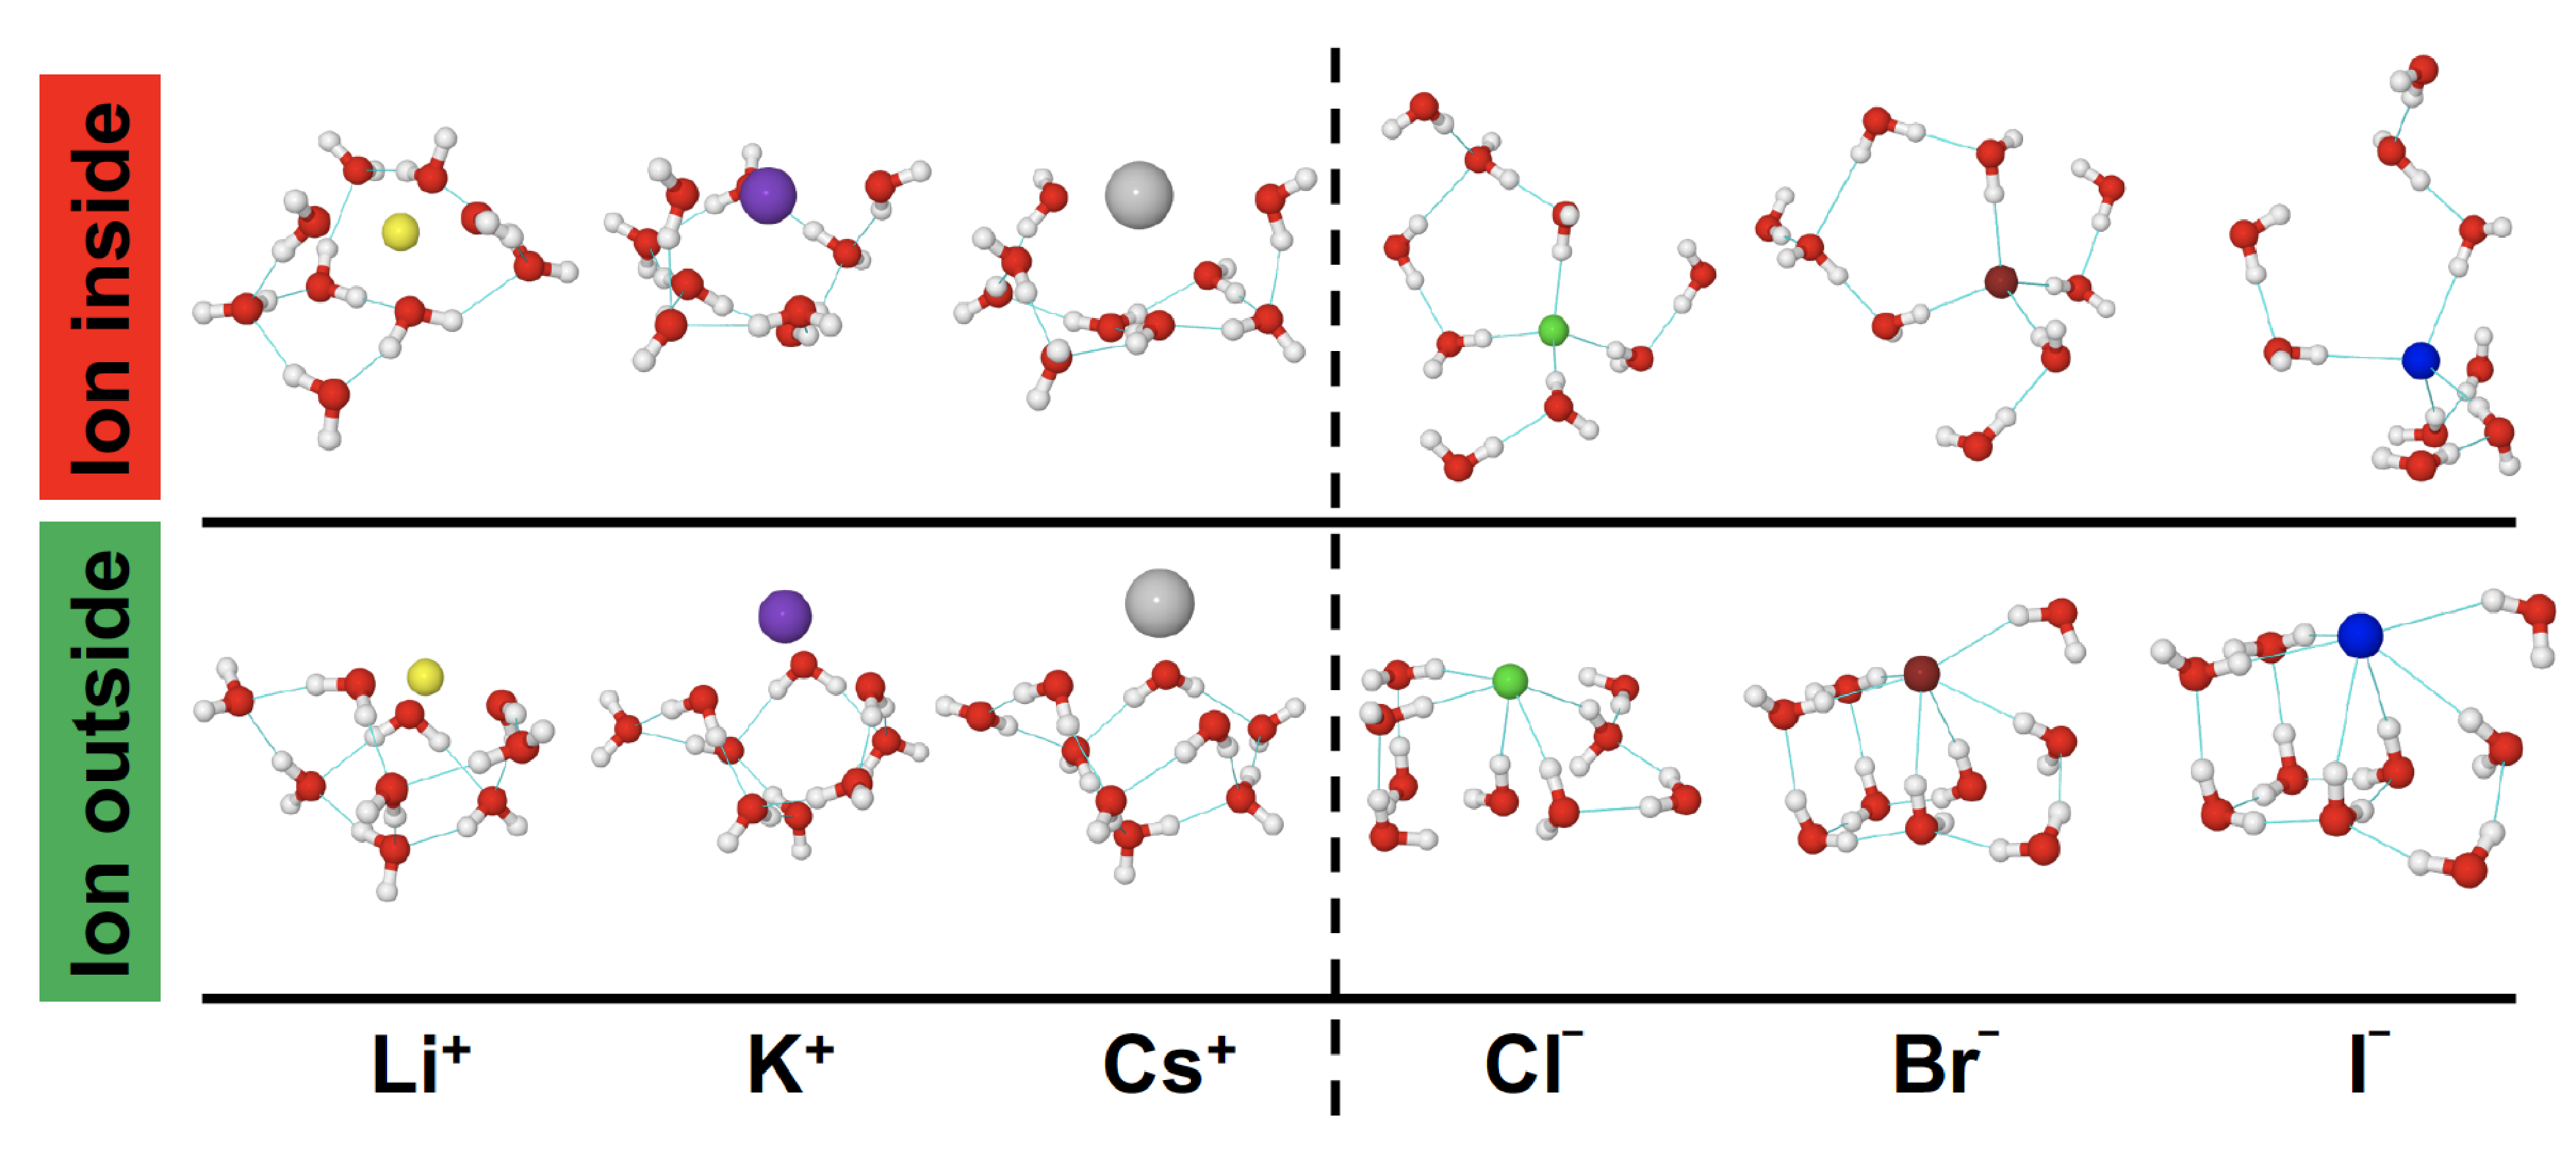
\includegraphics[width=\textwidth]{Figures/Chapter_3/figure_1.pdf}
\caption[temp]{Geometries of the ionic clusters used for the MBE calculation. For each ion, two different arrangements (ion inside, ion outside) were considered.}
\label{fig:MBE_II_1}
\end{figure}

\begin{figure}[t]
\uwsinglespace
\centering
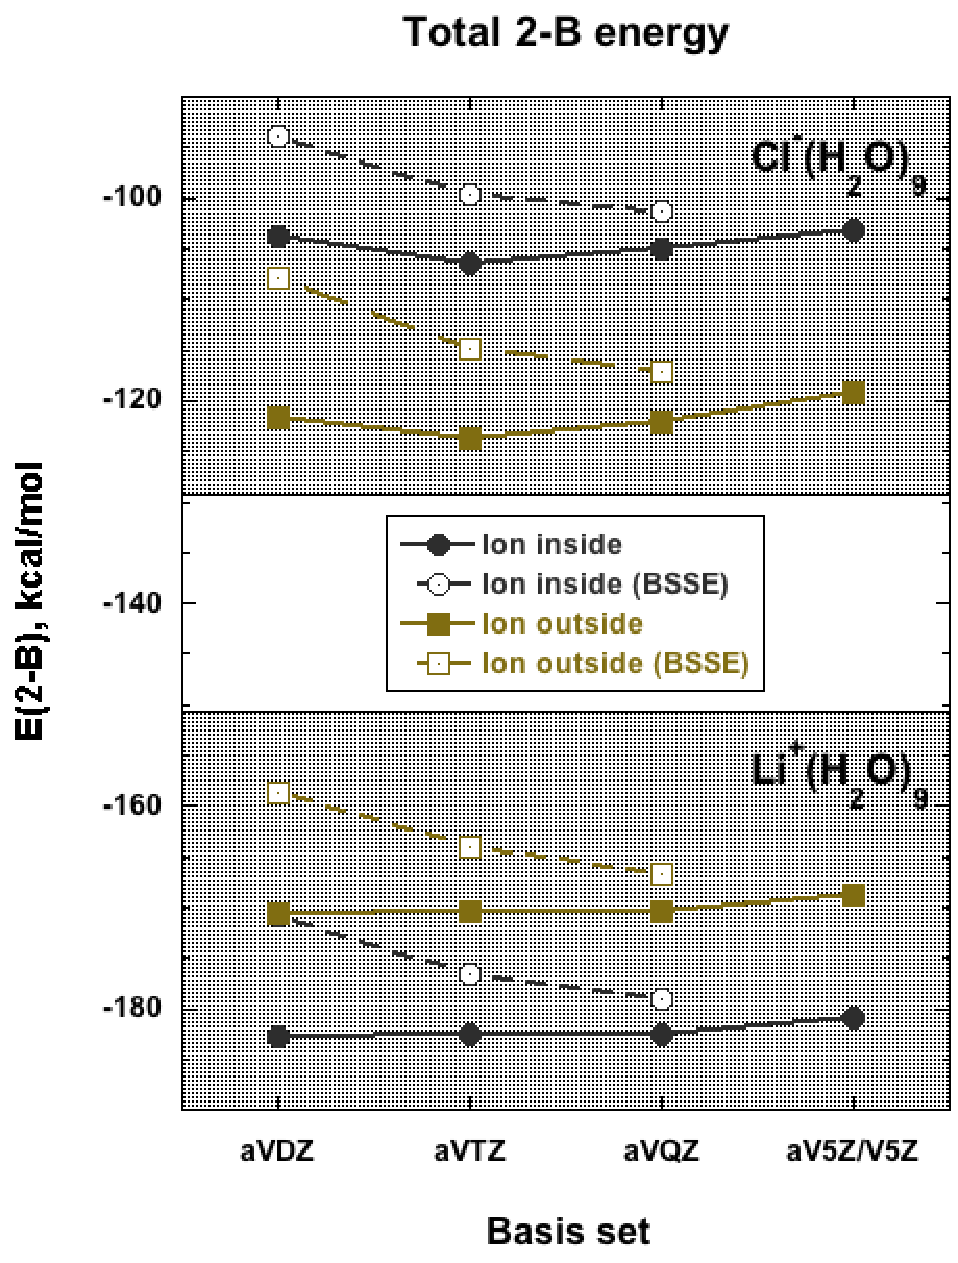
\includegraphics[width=\textwidth]{Figures/Chapter_3/figure_2.pdf}
\caption[temp]{Variation of the total uncorrected (filled symbols, solid lines) and BSSE-corrected (open symbols, dashed lines) 2-B energy with basis set for the ion inside and ion outside isomers of the \ce{Li^+(H2O)9} (lower shaded area) and \ce{Cl^-(H2O)9} (upper shaded area) clusters.}
\label{fig:MBE_II_2}
\end{figure}

\begin{figure}[t]
\uwsinglespace
\begin{center}
\begin{minipage}{0.45\textwidth}
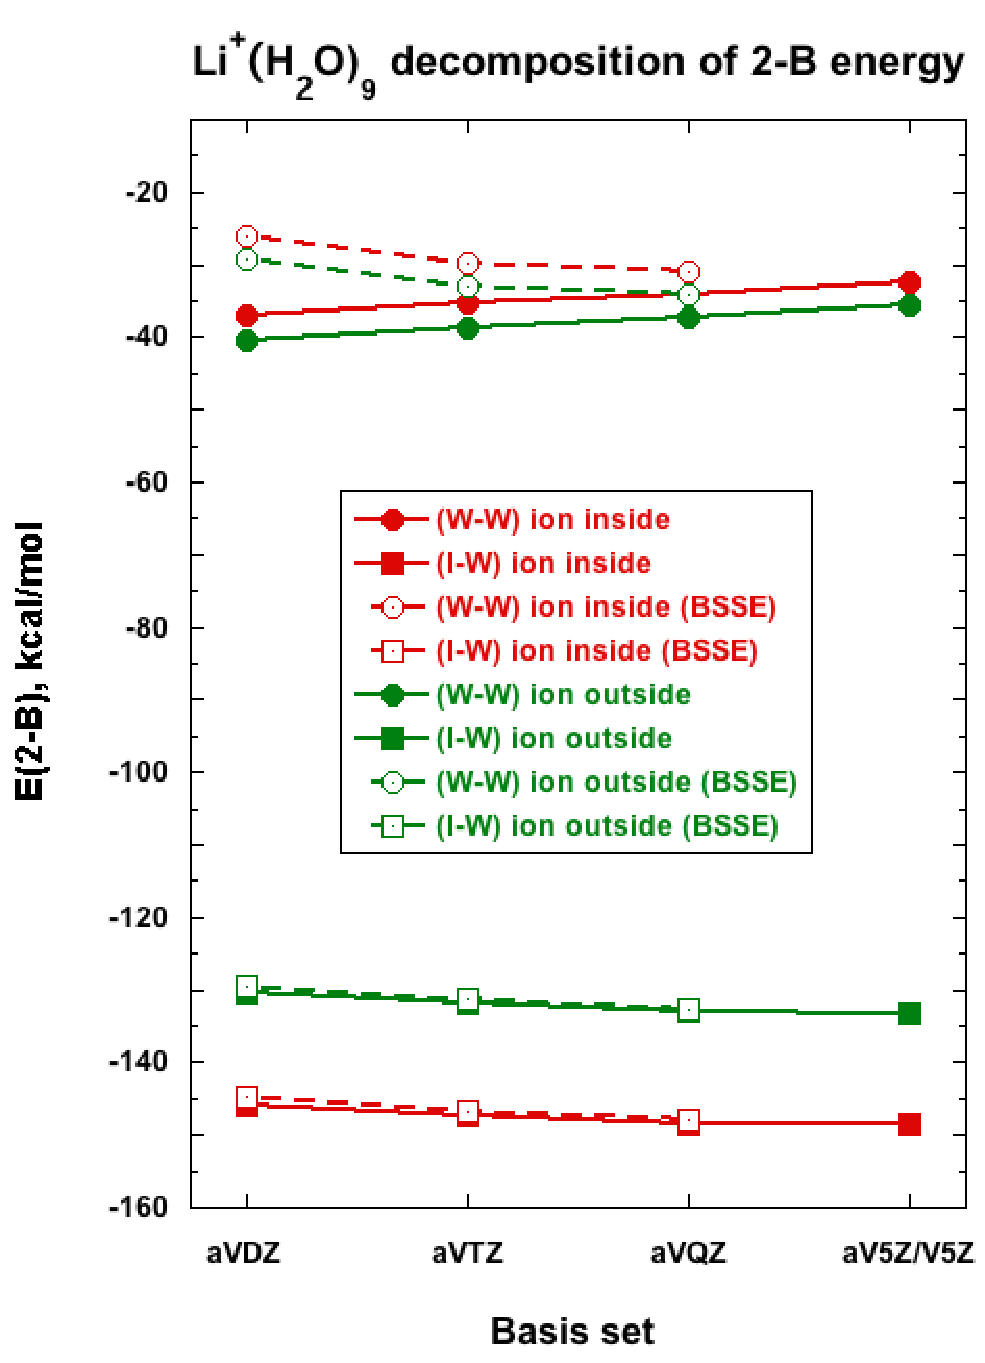
\includegraphics[width=.9\textwidth]{Figures/Chapter_3/figure_3_left.pdf}
\end{minipage}
\begin{minipage}{0.45\textwidth}
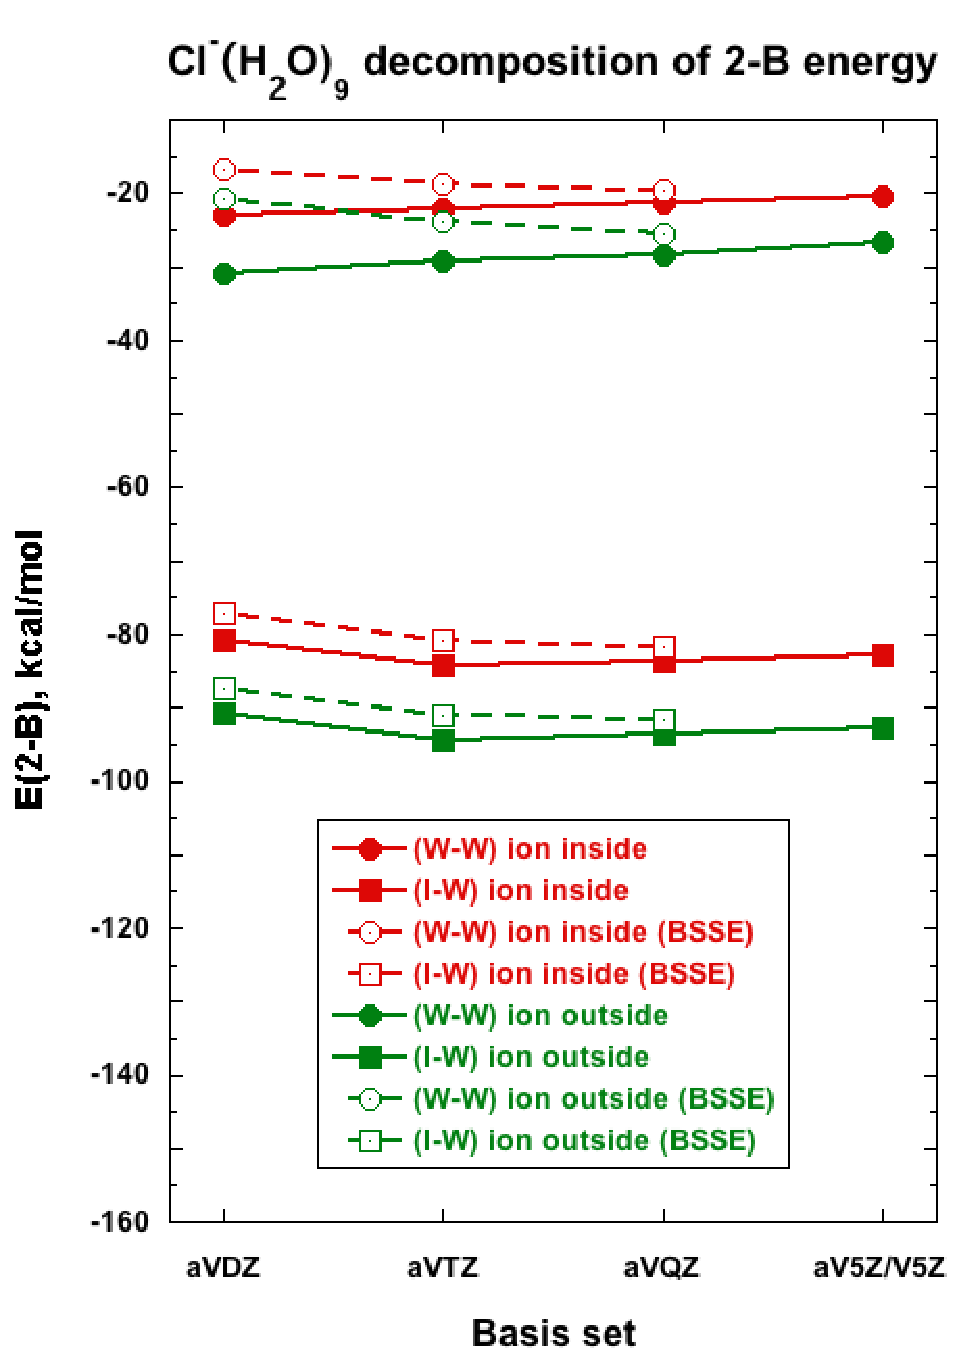
\includegraphics[width=.9\textwidth]{Figures/Chapter_3/figure_3_right.pdf}
\end{minipage}
\end{center}
\caption[temp]{Magnitude of the individual ion-water (I-W) and water-water (W-W) 2-Body energy terms with (open symbols) and without (filled symbols) BSSE correction for the ion inside (red) and ion outside (green) configurations of the \ce{Li^+(H2O)9} (left panel) and \ce{Cl^-(H2O)9} (right panel) clusters. Notice the same y-axis scales.}
\label{fig:MBE_II_3}
\end{figure}

\begin{figure}[t]
\uwsinglespace
\centering
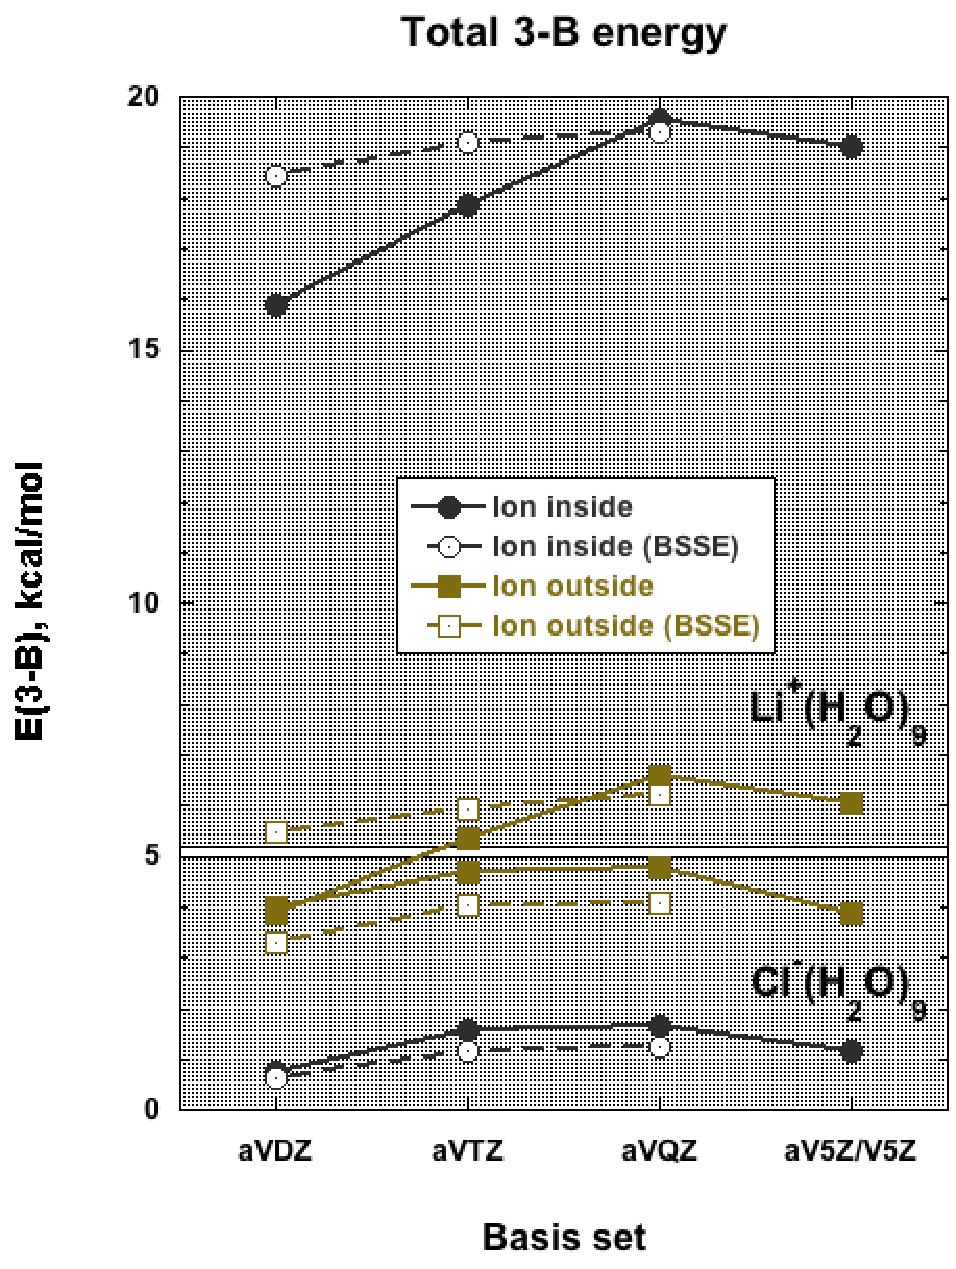
\includegraphics[width=\textwidth]{Figures/Chapter_3/figure_4.pdf}
\caption[temp]{Variation of the total uncorrected (filled symbols, solid lines) and BSSE-corrected (open symbols, dashed lines) 3-B energy with basis set for the ion inside and ion outside isomers of the \ce{Li^+(H2O)9} (upper shaded area) and \ce{Cl^-(H2O)9} (lower shaded area) clusters.}
\label{fig:MBE_II_4}
\end{figure}

\begin{figure}[t]
\uwsinglespace
\begin{center}
\begin{minipage}{0.45\textwidth}
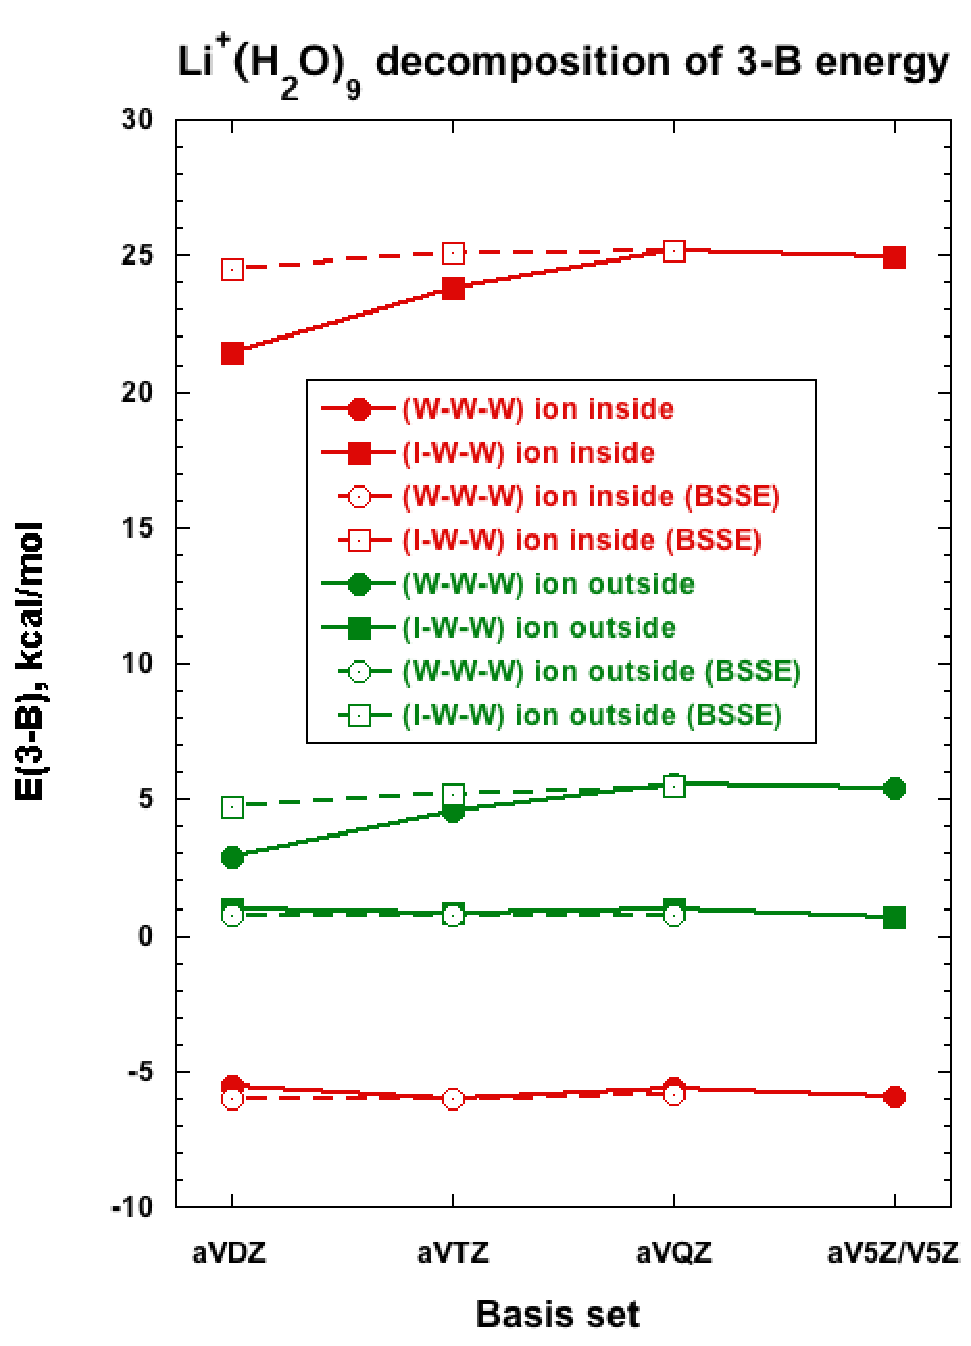
\includegraphics[width=.9\textwidth]{Figures/Chapter_3/figure_5_left.pdf}
\end{minipage}
\begin{minipage}{0.45\textwidth}
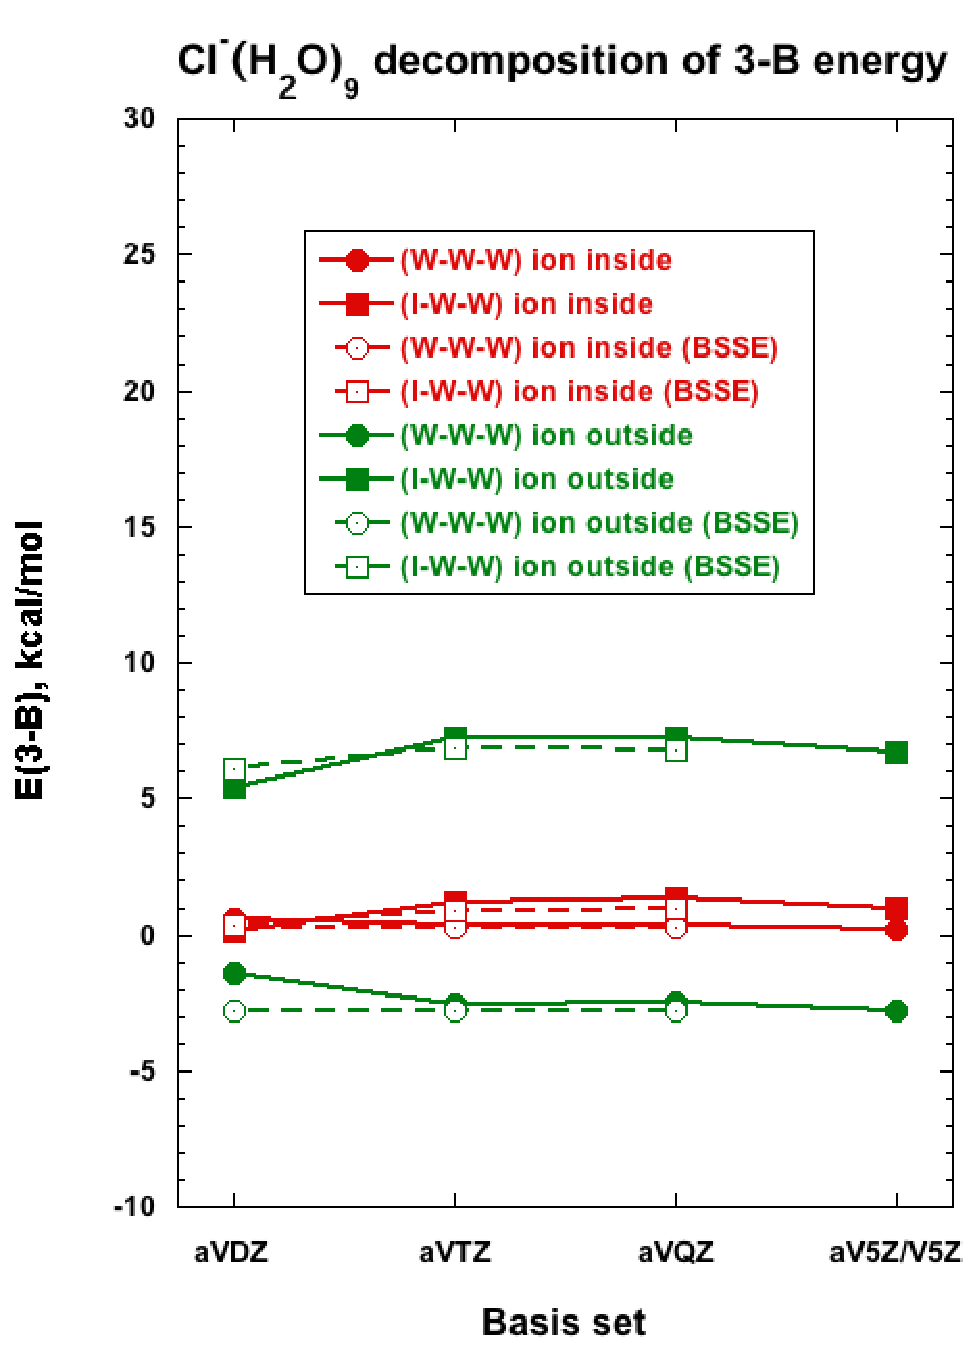
\includegraphics[width=.9\textwidth]{Figures/Chapter_3/figure_5_right.pdf}
\end{minipage}
\end{center}
\caption[temp]{Magnitude of the 3-Body energy with and without BSSE correction for \ce{Cl^-(H2O)9} (left) and \ce{Li^+(H2O)9} (right) split into contributions from ion-water-water interactions and water-water-water interactions. Notice the same y-axis scales.}
\label{fig:MBE_II_5}
\end{figure}

\begin{figure}[t]
\uwsinglespace
\centering
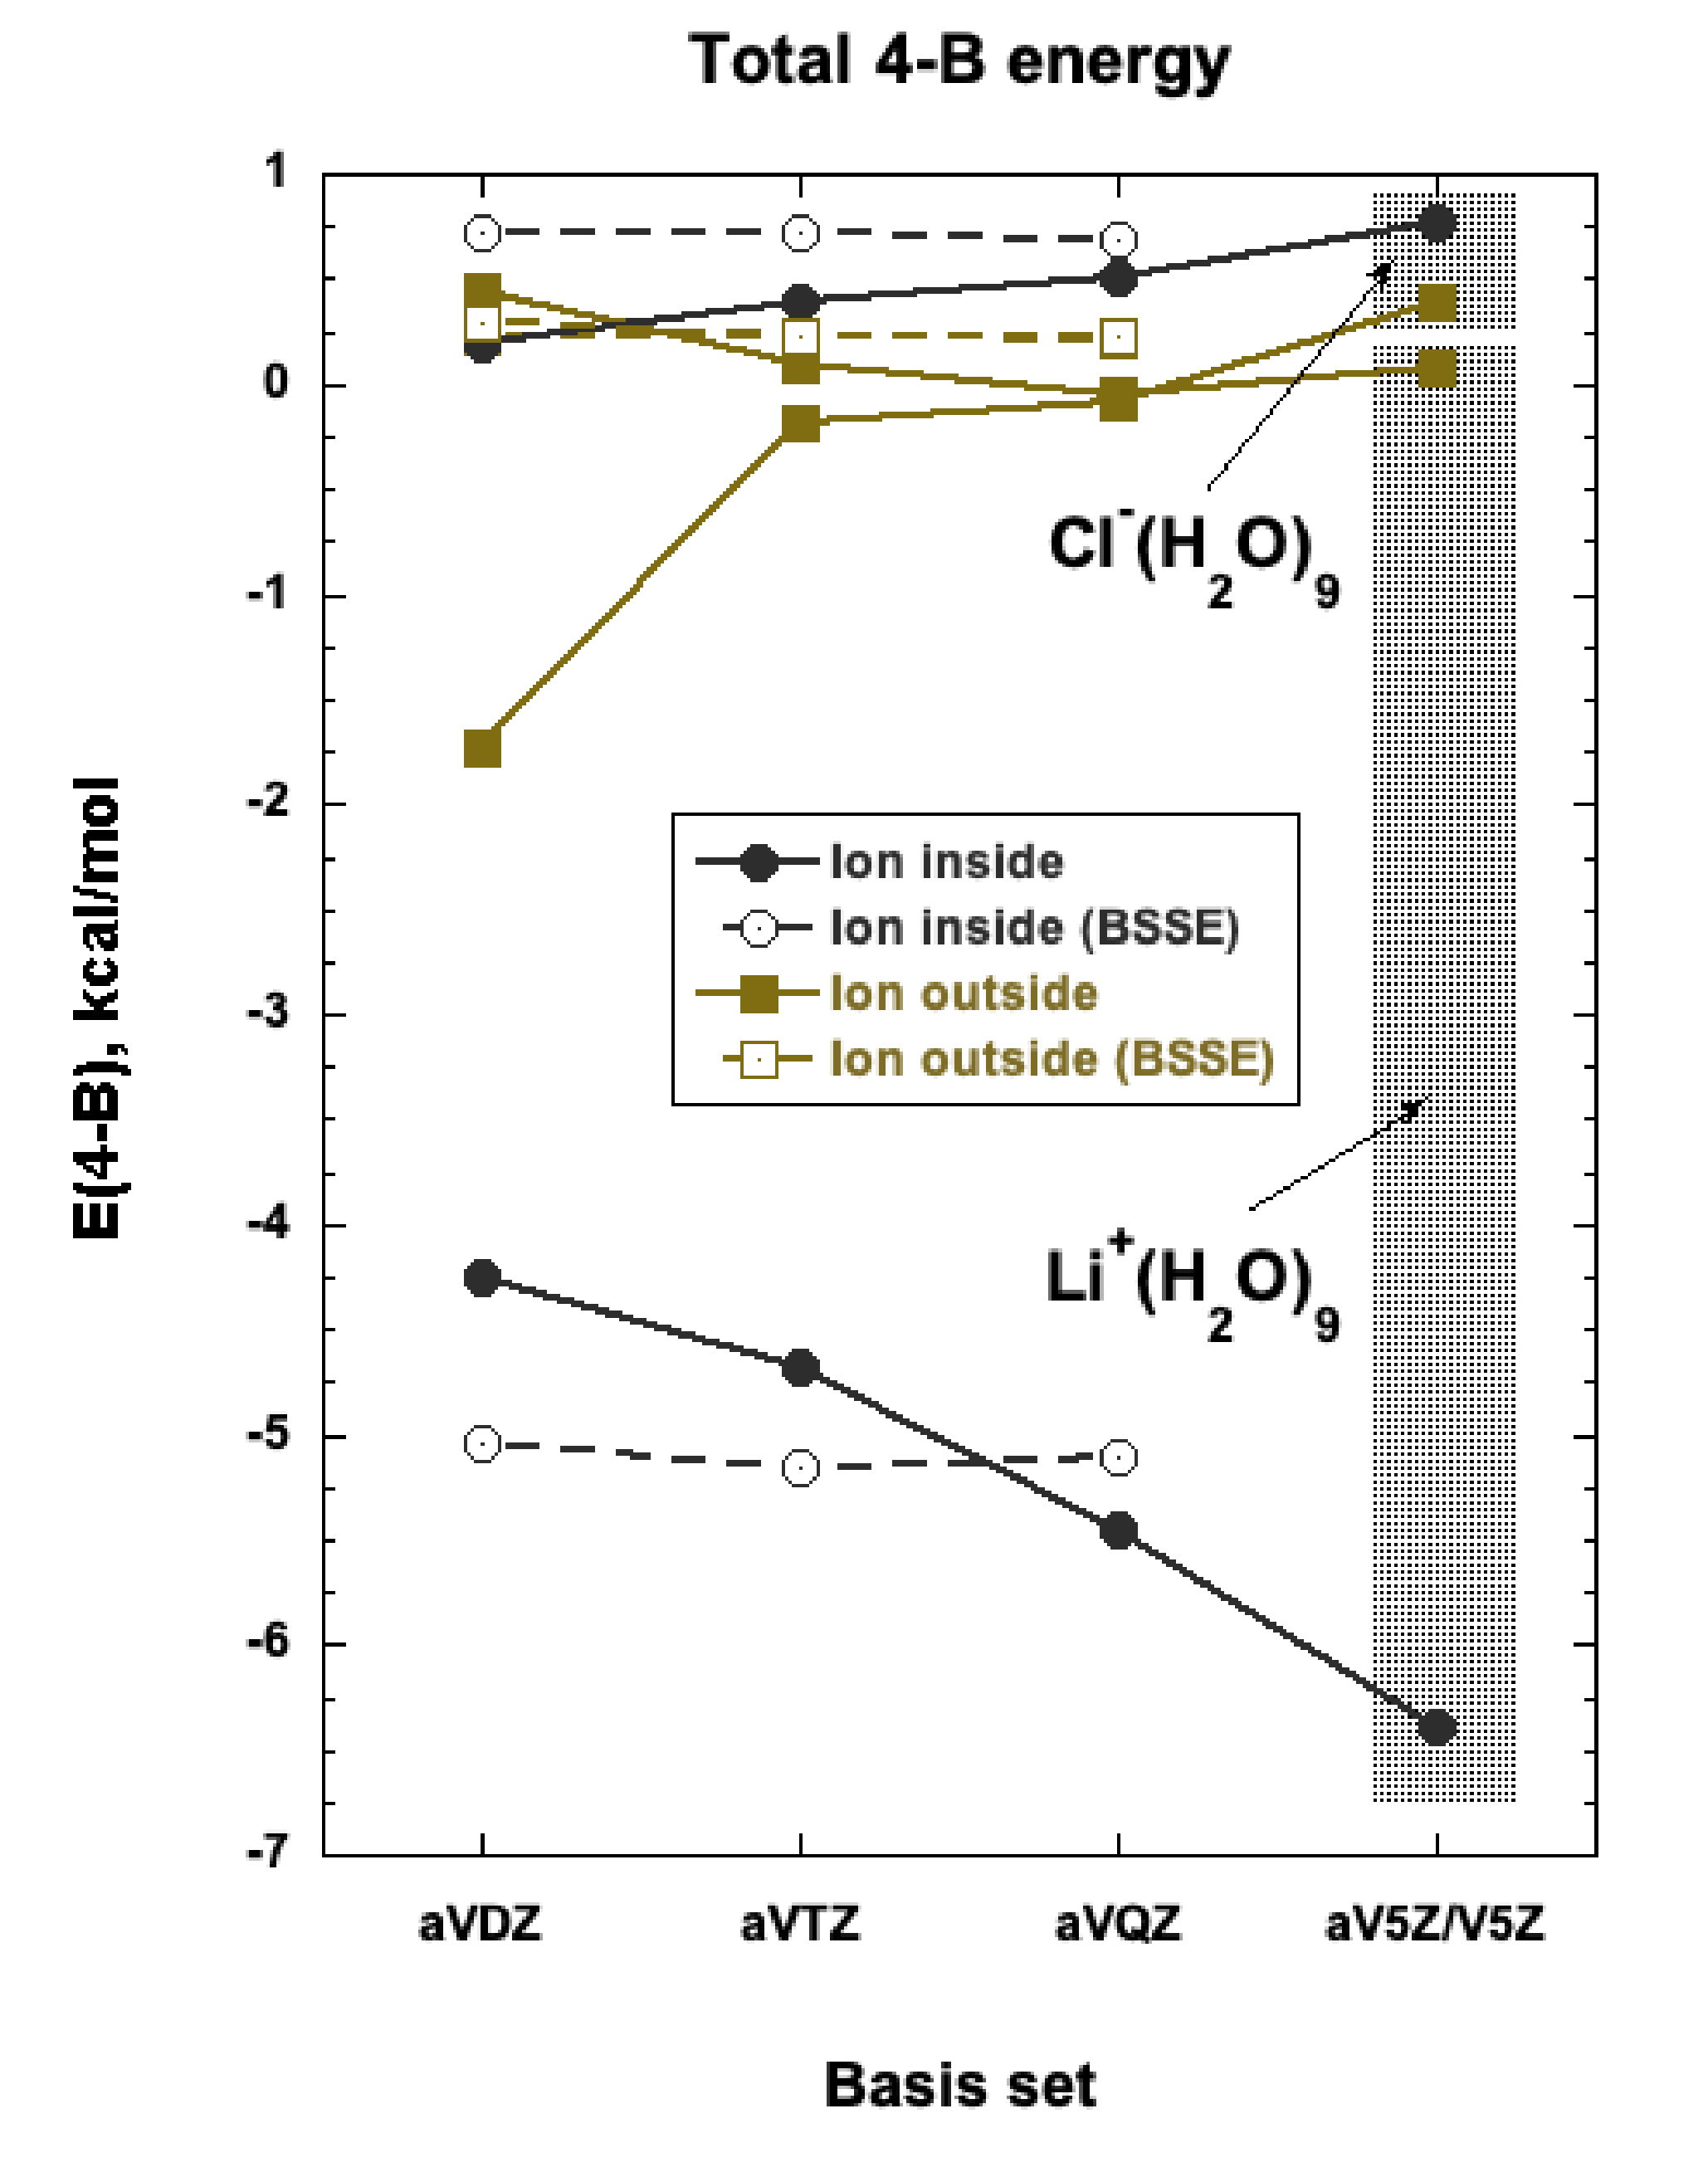
\includegraphics[width=\textwidth]{Figures/Chapter_3/figure_6.pdf}
\caption[temp]{Variation of the total uncorrected (filled symbols, solid lines) and BSSE-corrected (open symbols, dashed lines) 4-B energy with basis set for the ion inside and ion outside isomers of the \ce{Li^+(H2O)9} (lower shaded area) and \ce{Cl^-(H2O)9} (upper shaded area) clusters.}
\label{fig:MBE_II_6}
\end{figure}

\begin{figure}
  \begin{subfigure}[t]{.5\textwidth}
    \centering
    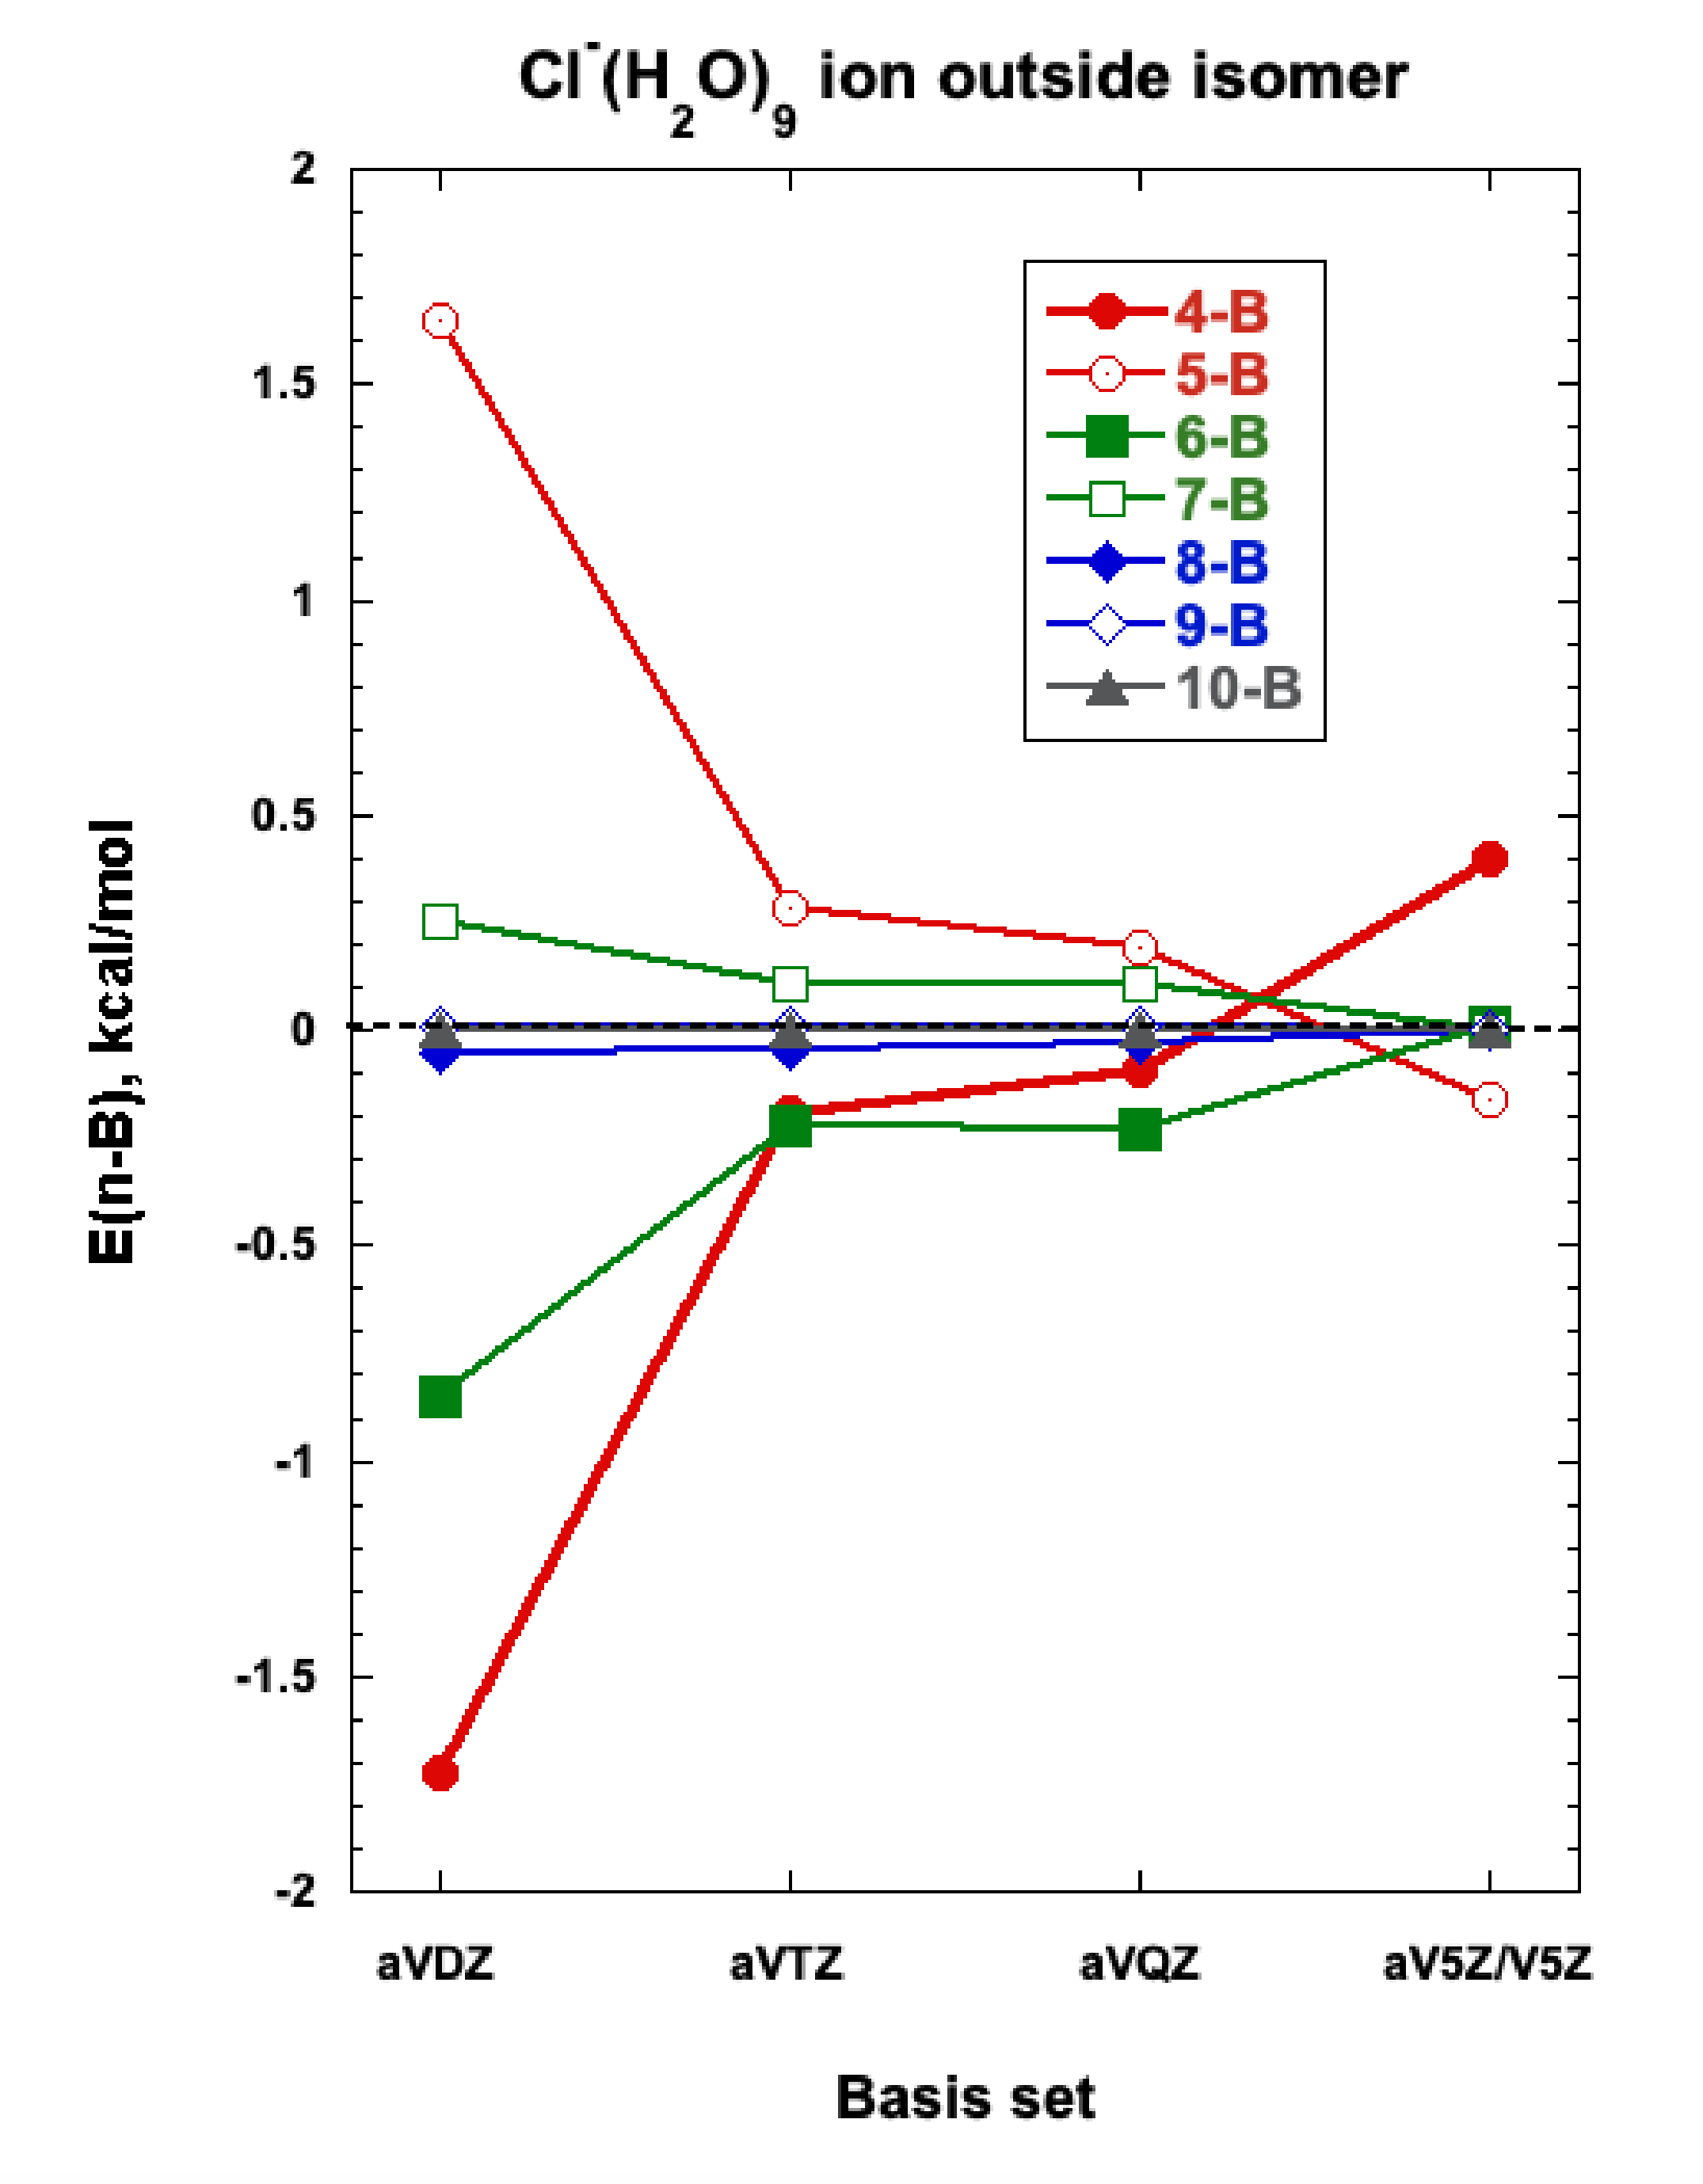
\includegraphics[width=\linewidth]{Figures/Chapter_3/figure_7_tl.pdf}
  \end{subfigure}
  \hfill
  \begin{subfigure}[t]{.5\textwidth}
    \centering
    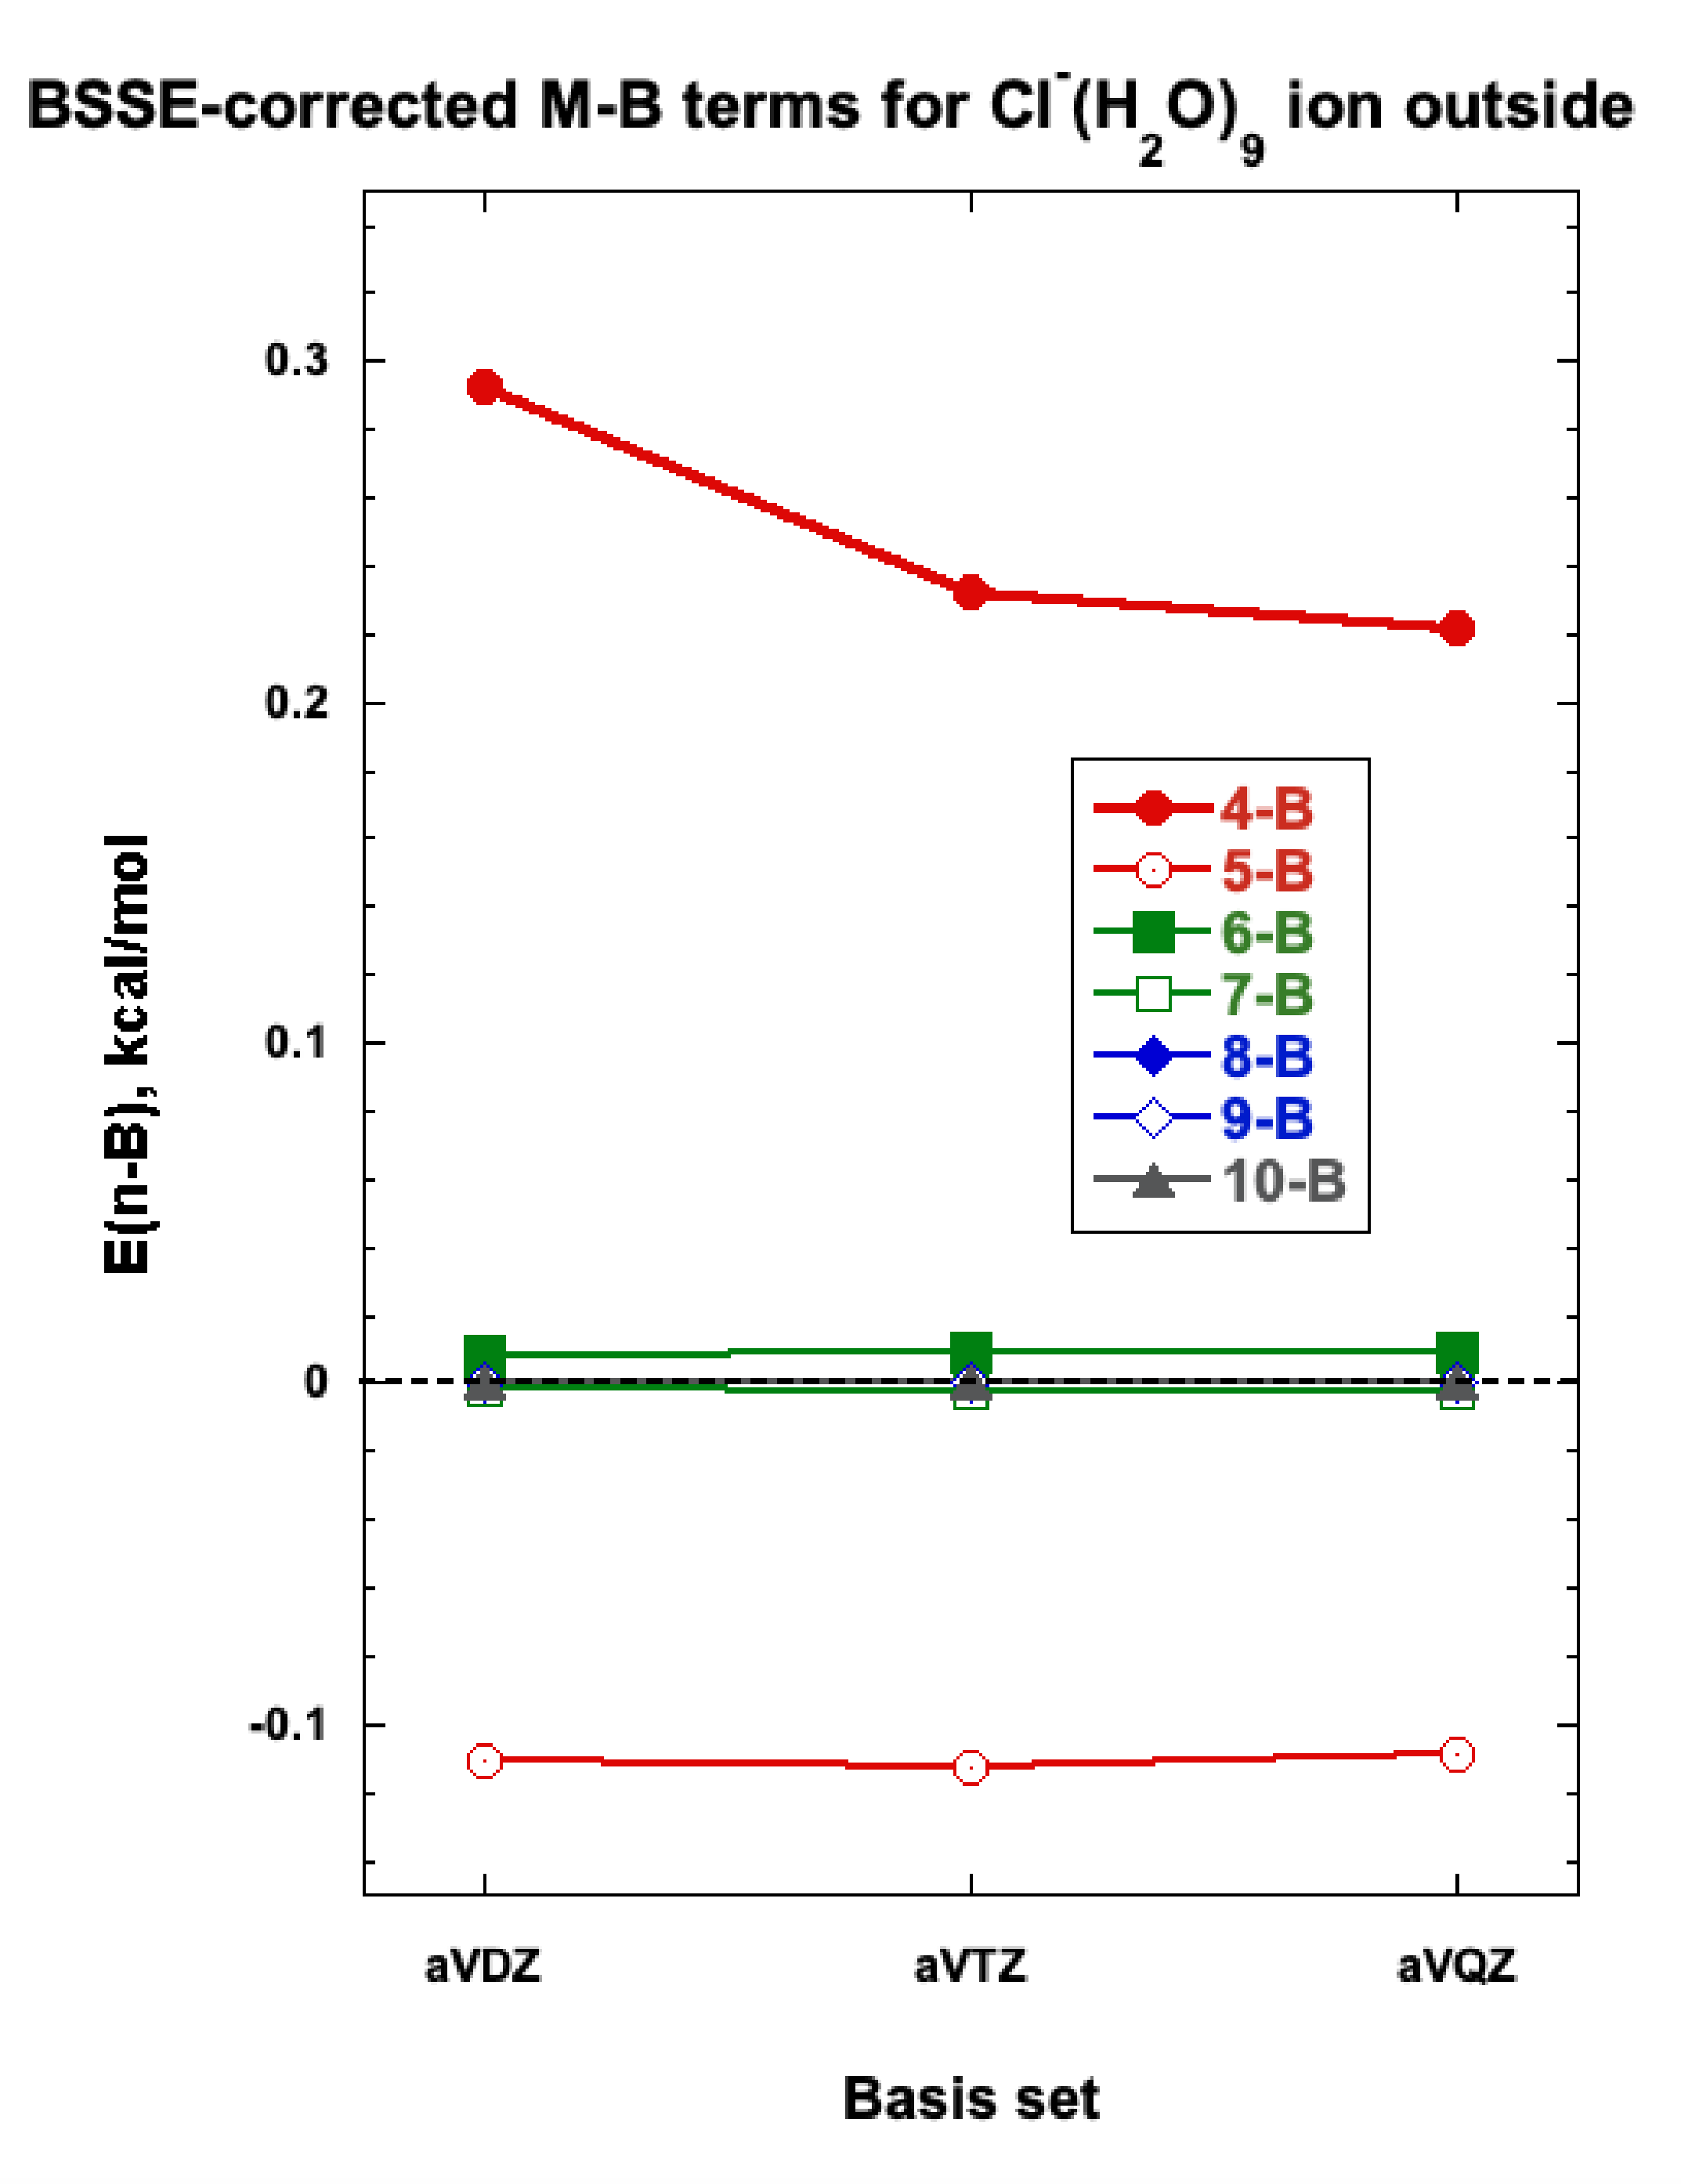
\includegraphics[width=\linewidth]{Figures/Chapter_3/figure_7_tr.pdf}
  \end{subfigure}

  \medskip

  \begin{subfigure}[t]{.5\textwidth}
    \centering
    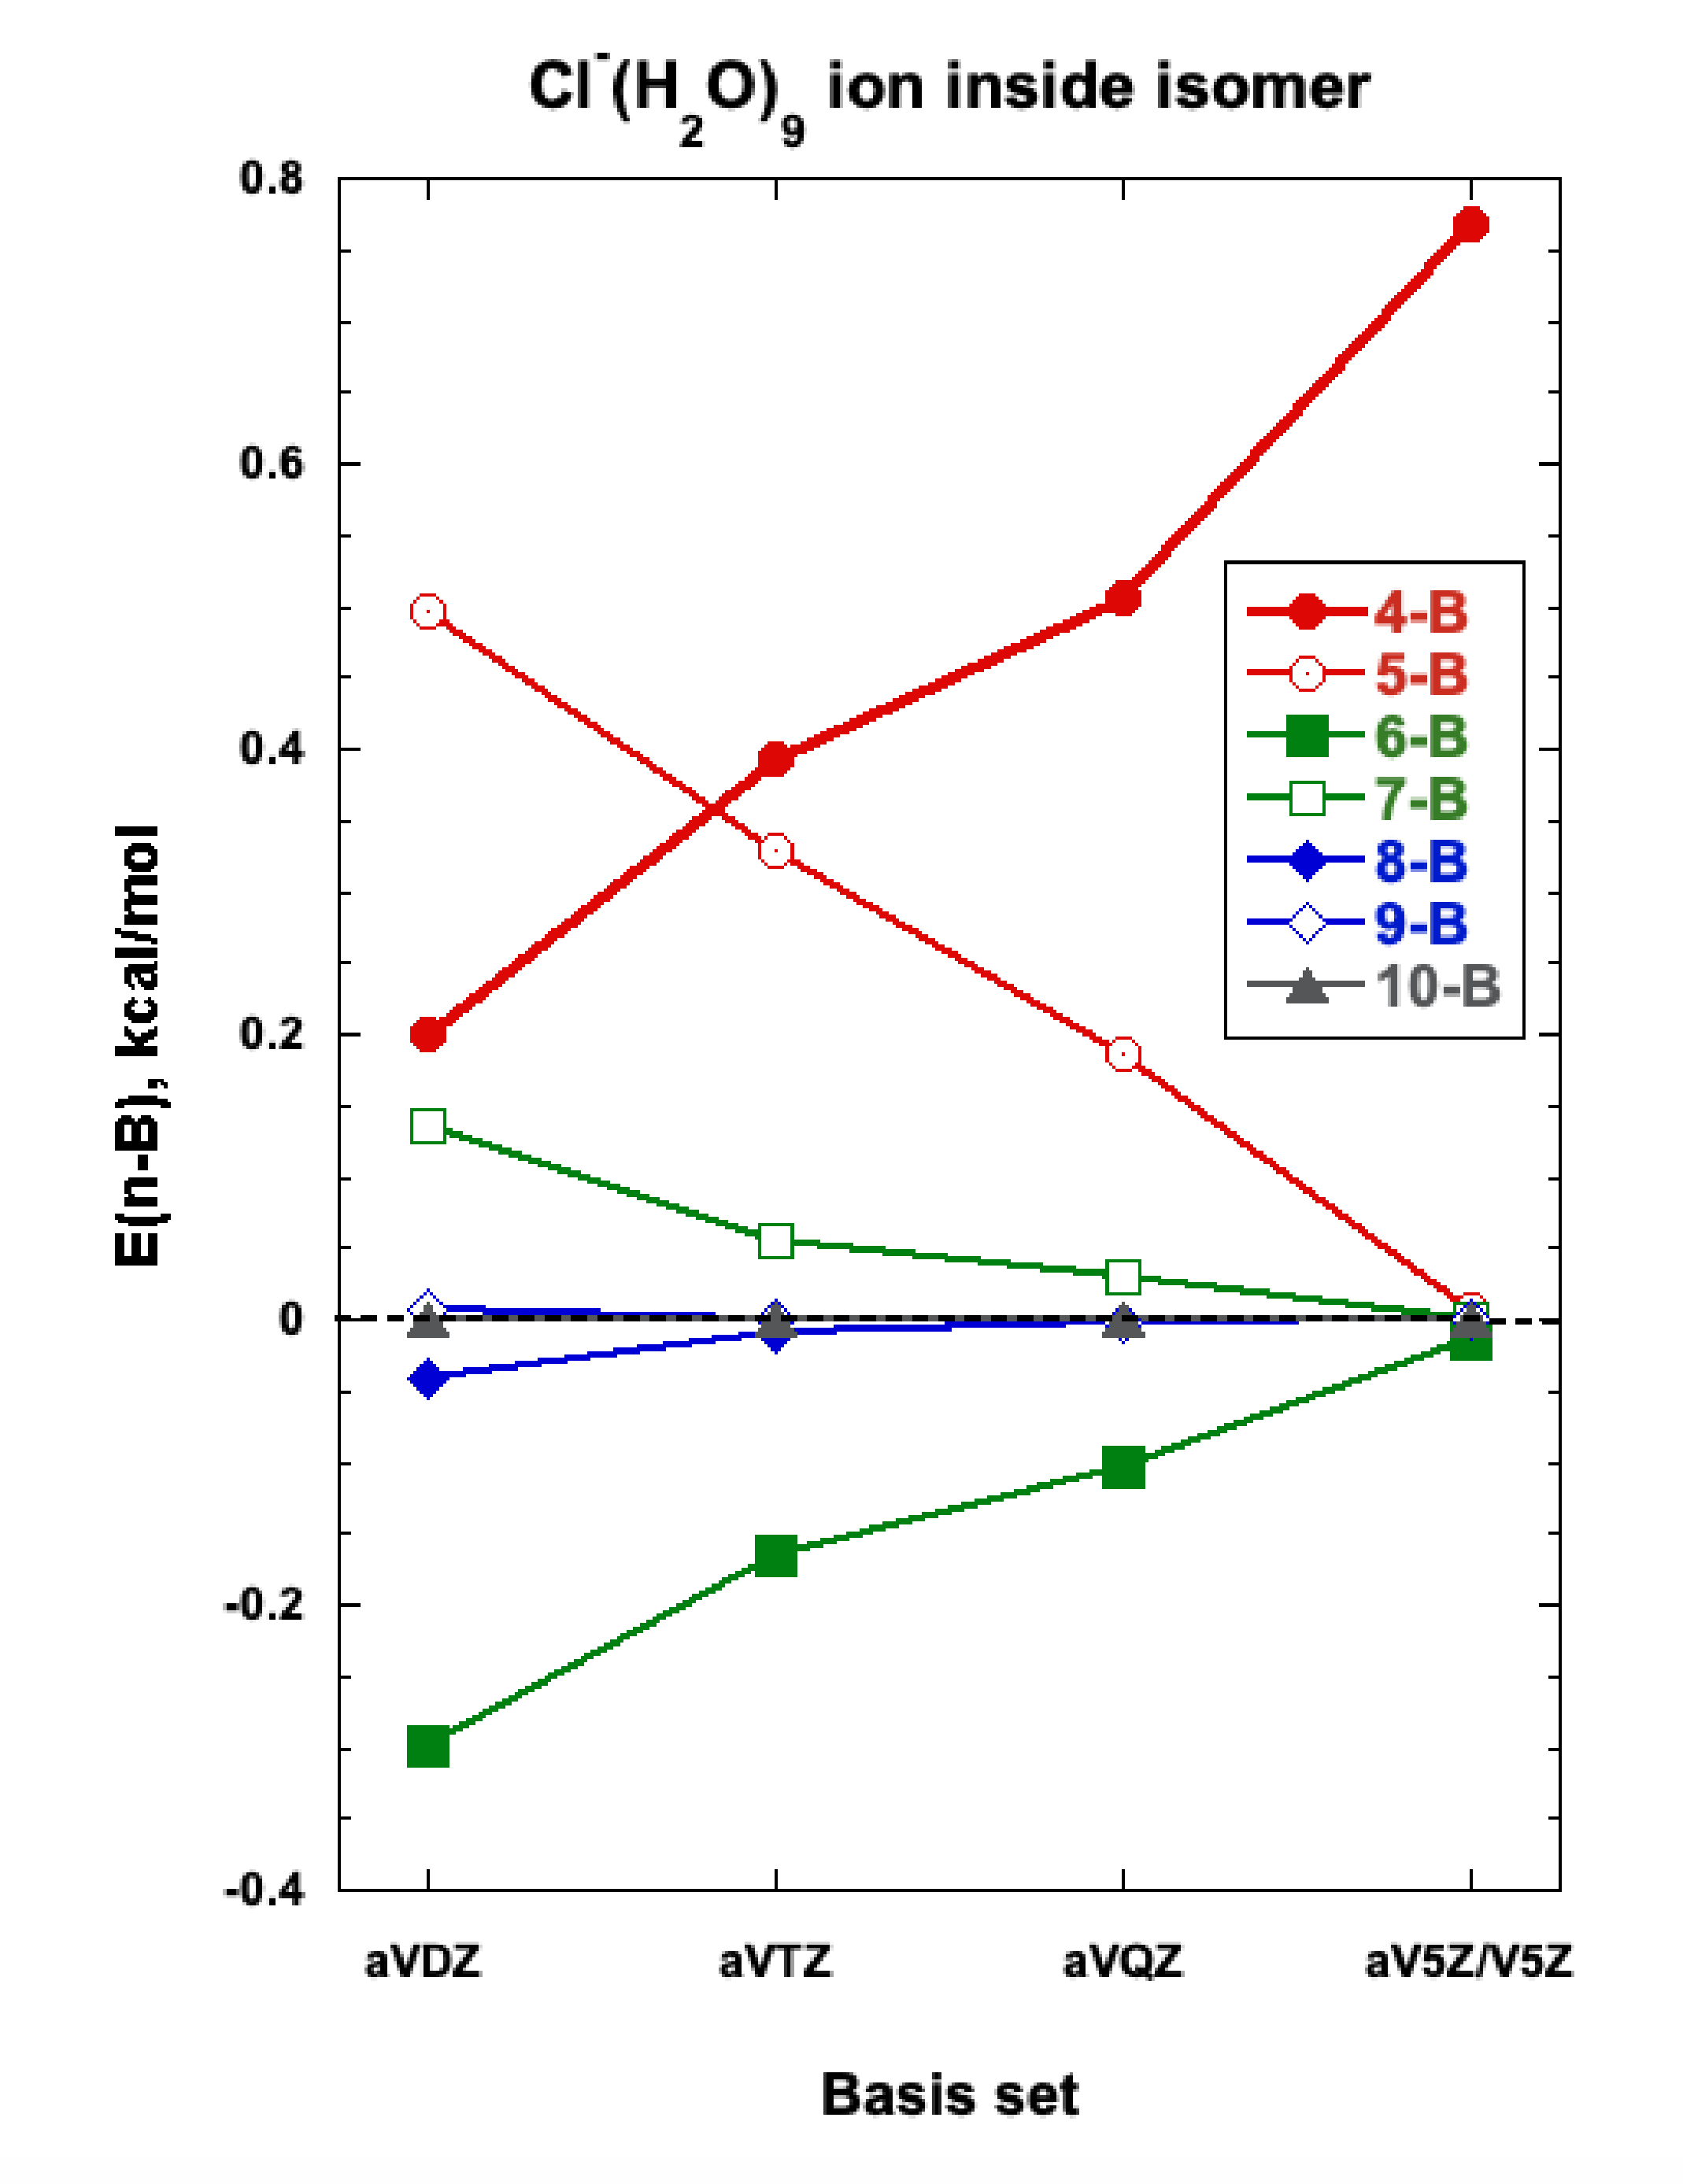
\includegraphics[width=\linewidth]{Figures/Chapter_3/figure_7_bl.pdf}
  \end{subfigure}
  \hfill
  \begin{subfigure}[t]{.5\textwidth}
    \centering
    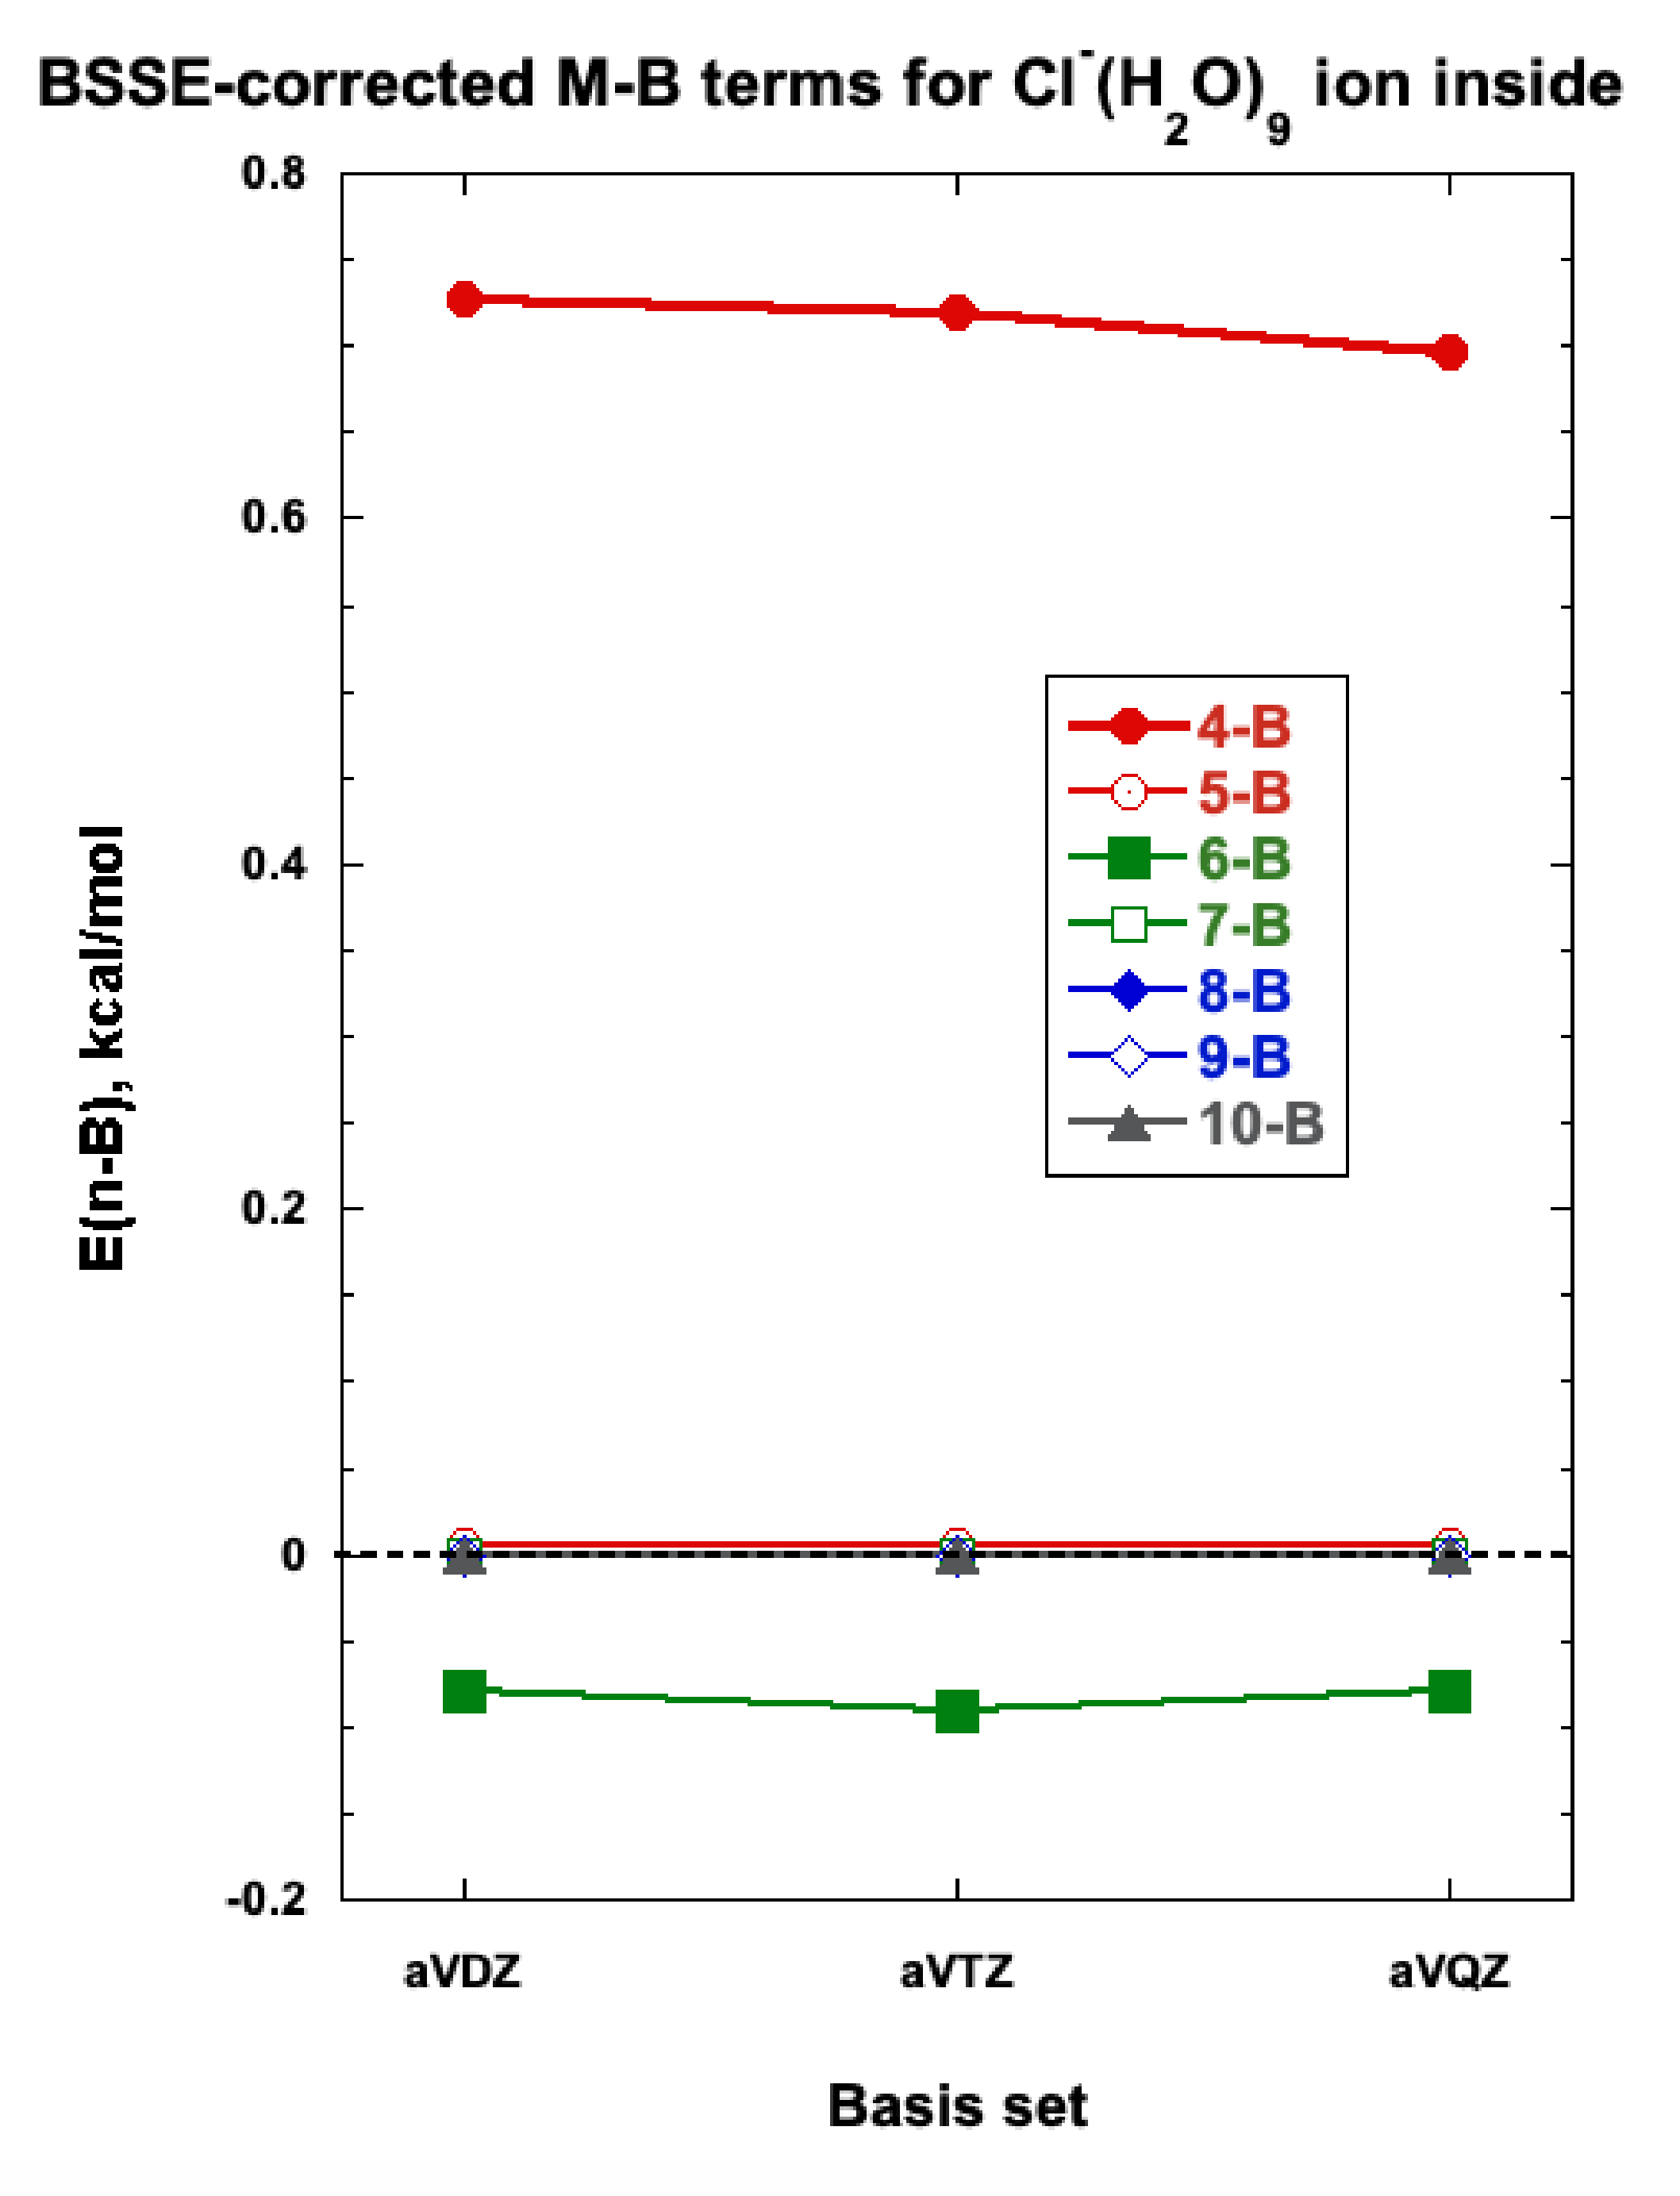
\includegraphics[width=\linewidth]{Figures/Chapter_3/figure_7_br.pdf}
  \end{subfigure}
  \caption{Many-body terms for \ce{Li^+(H2O)9}. Notice the different y-axis scales.}
  \label{fig:MBE_II_7}
\end{figure}

\begin{figure}
  \begin{subfigure}[t]{.5\textwidth}
    \centering
    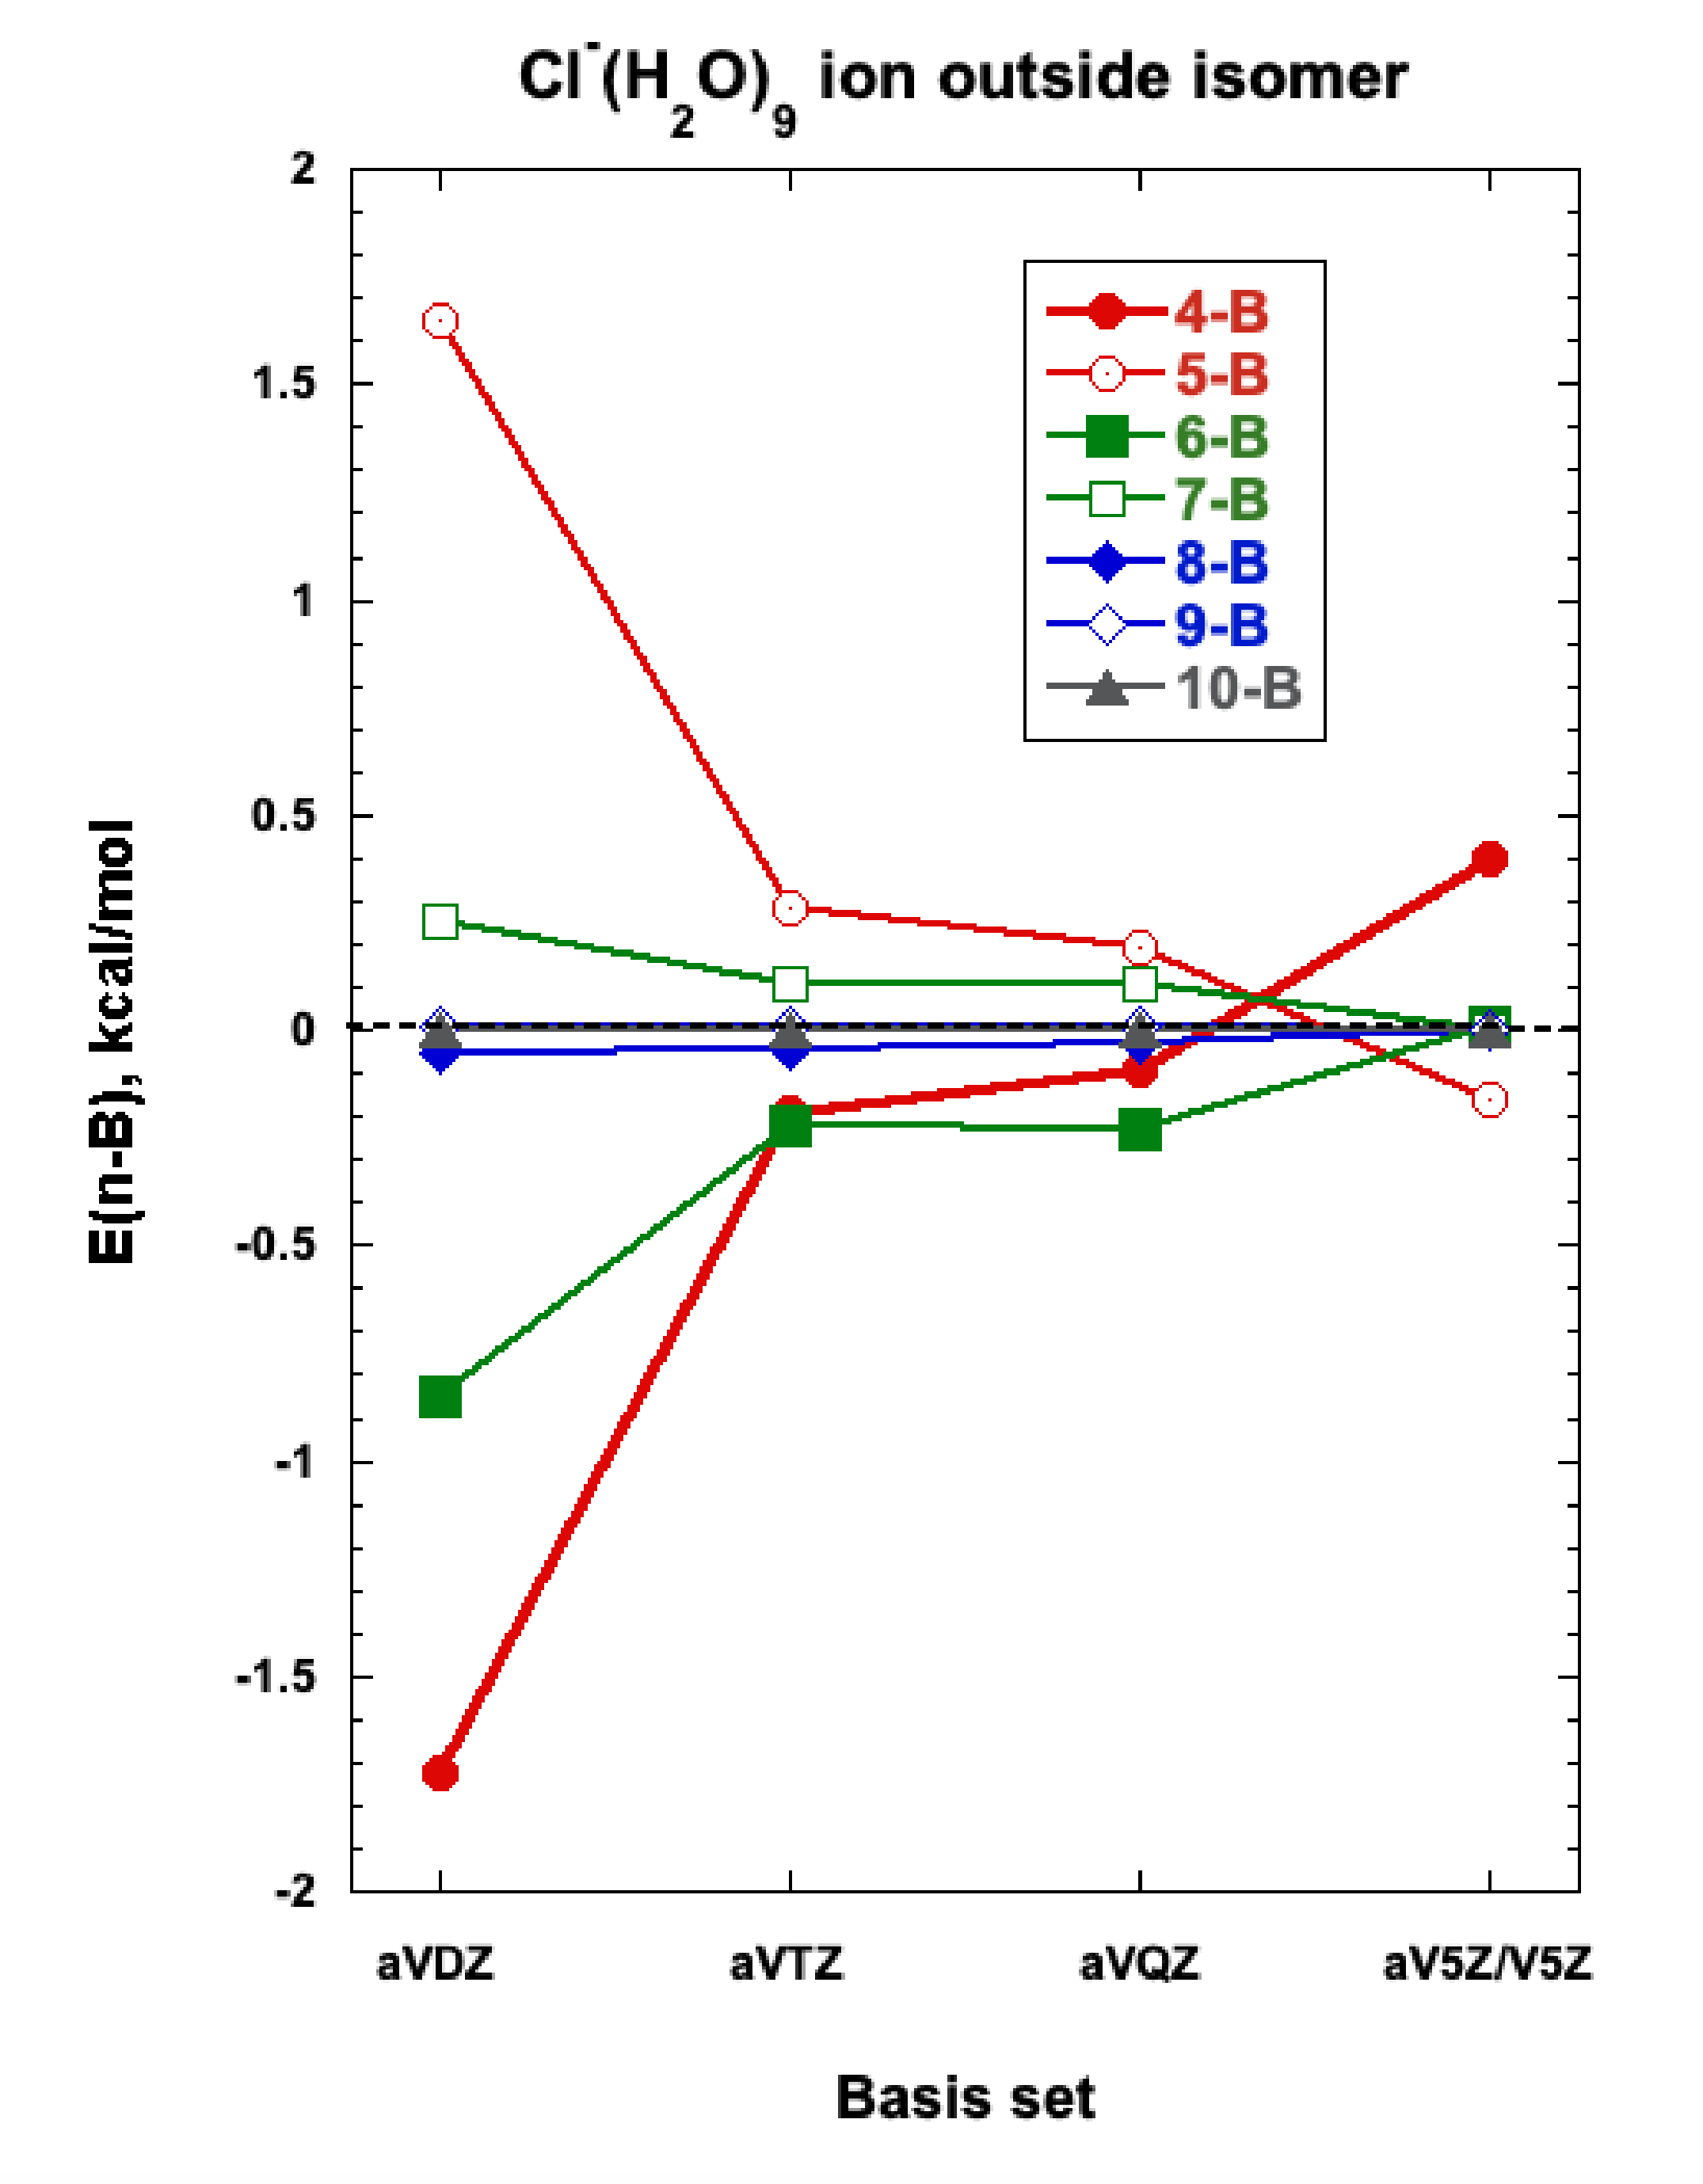
\includegraphics[width=\linewidth]{Figures/Chapter_3/figure_8_tl.pdf}
  \end{subfigure}
  \hfill
  \begin{subfigure}[t]{.5\textwidth}
    \centering
    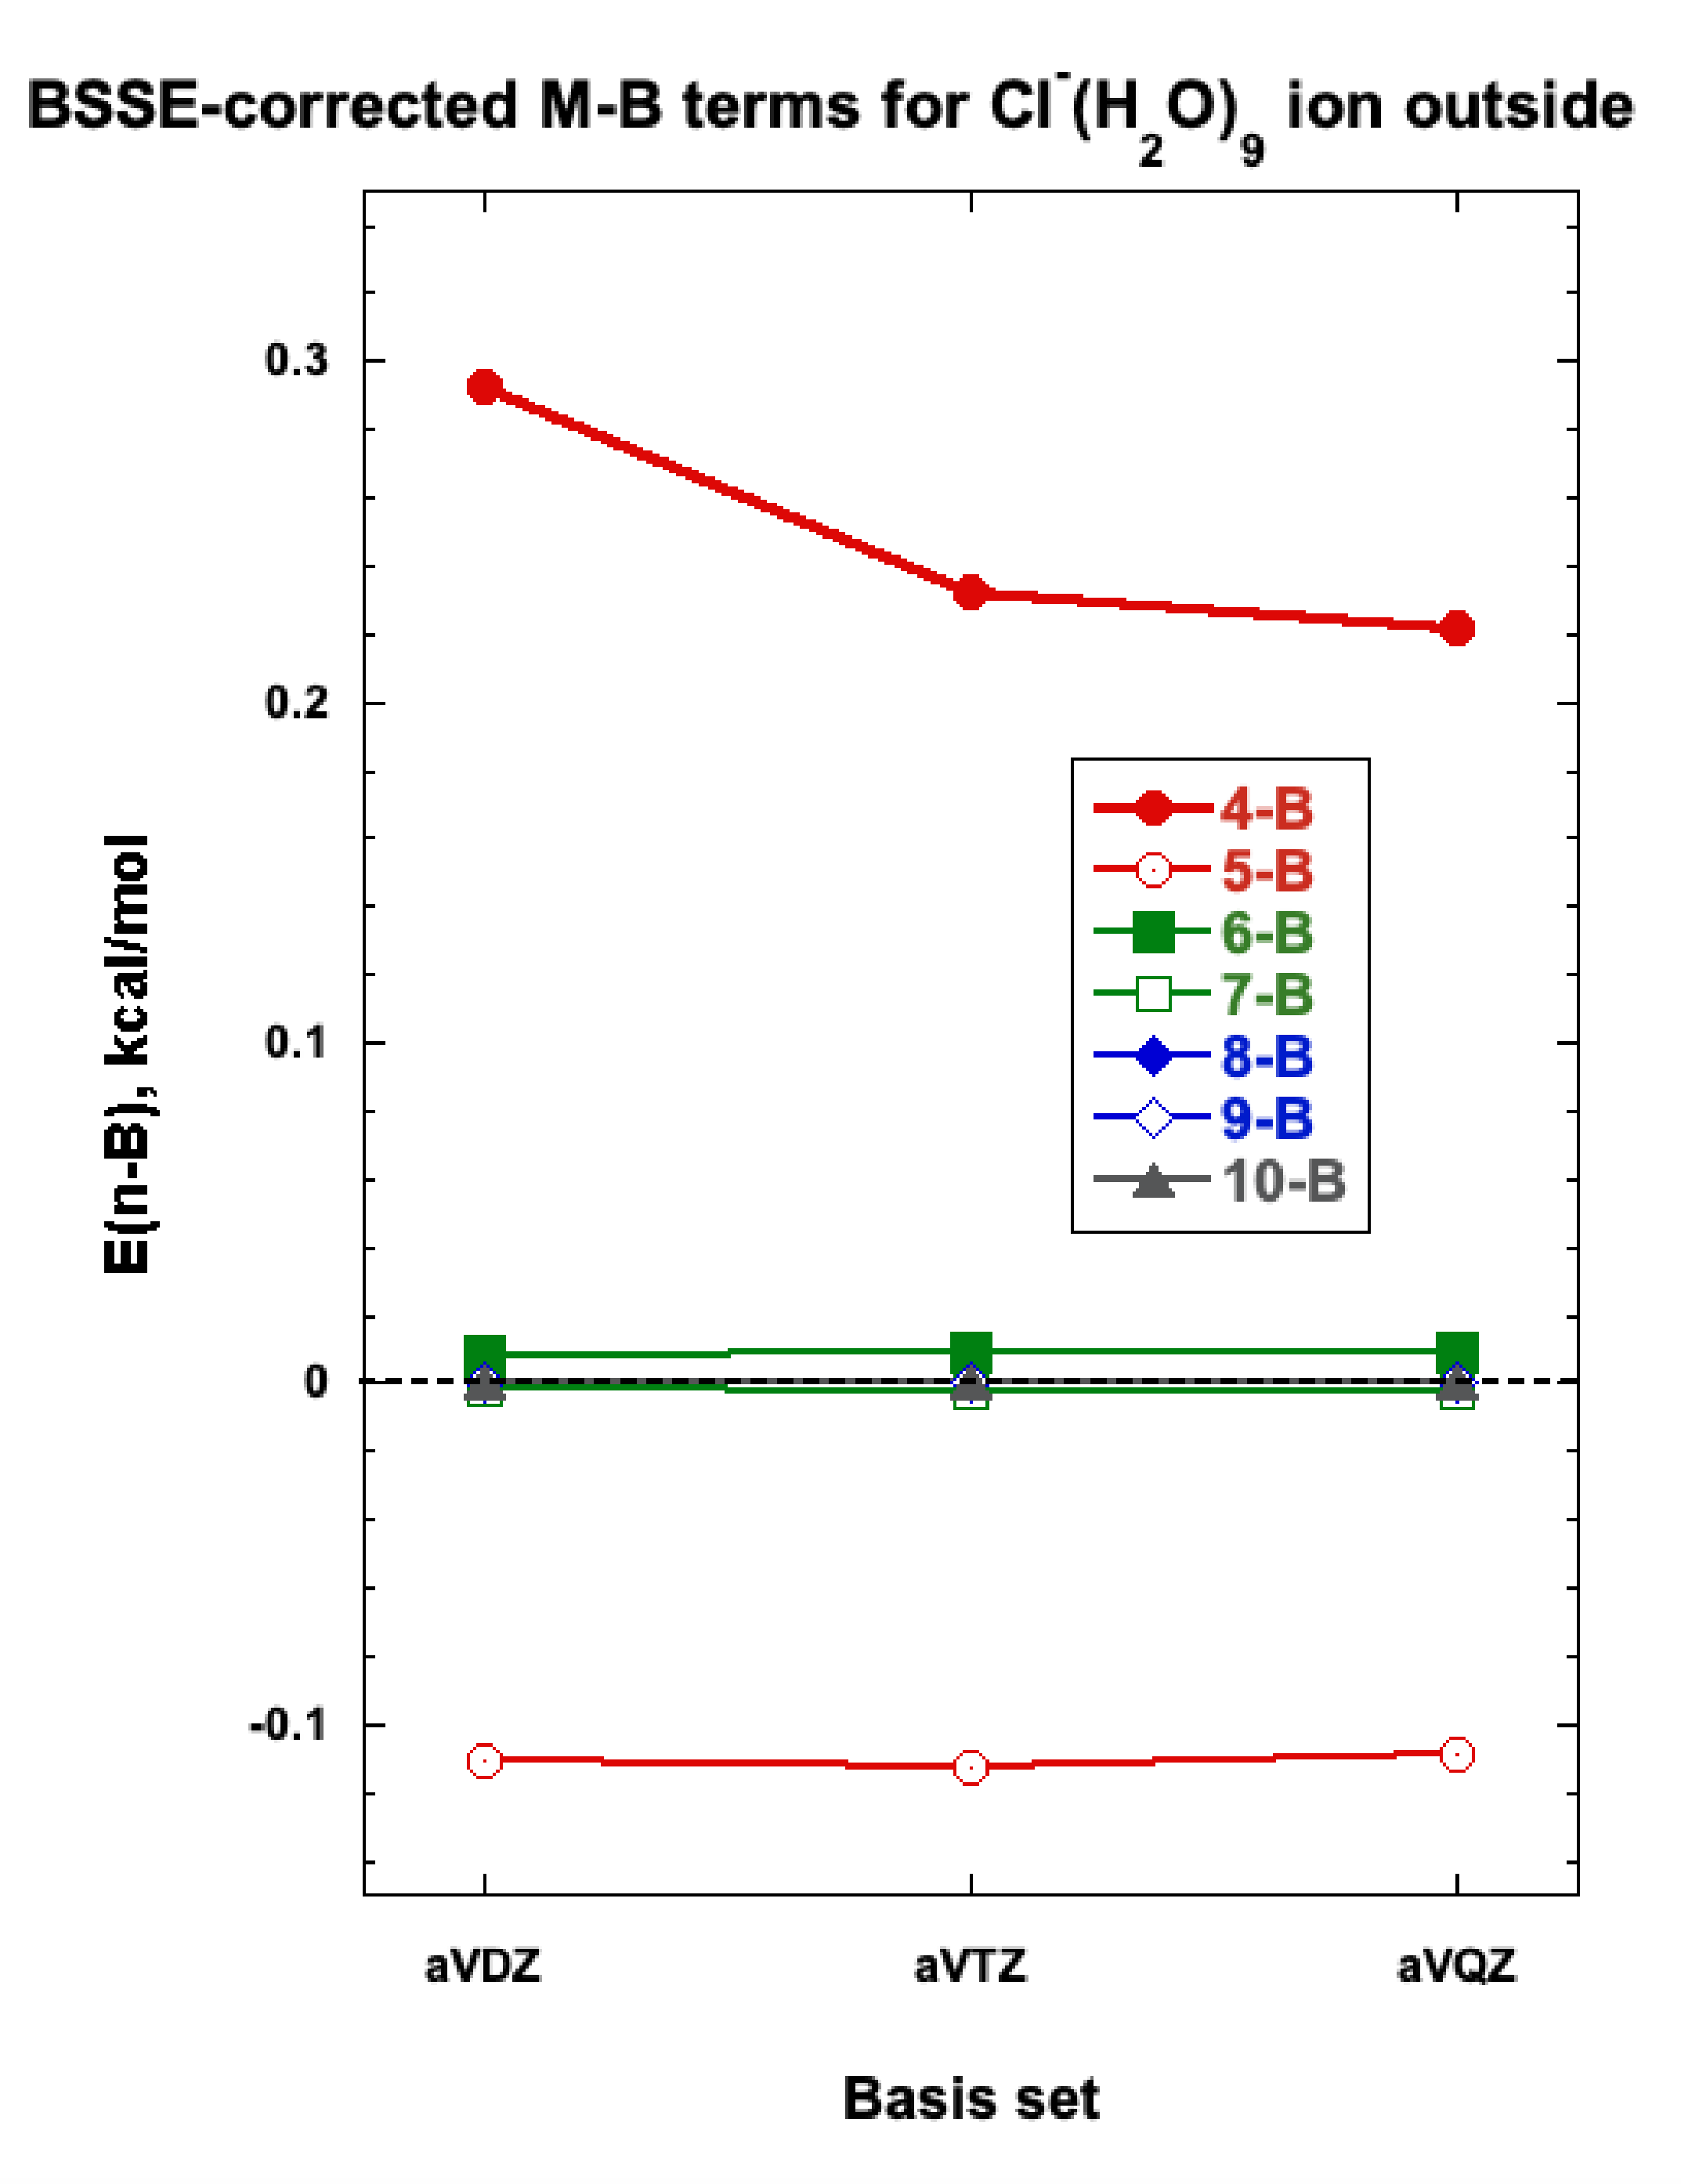
\includegraphics[width=\linewidth]{Figures/Chapter_3/figure_8_tr.pdf}
  \end{subfigure}

  \medskip

  \begin{subfigure}[t]{.5\textwidth}
    \centering
    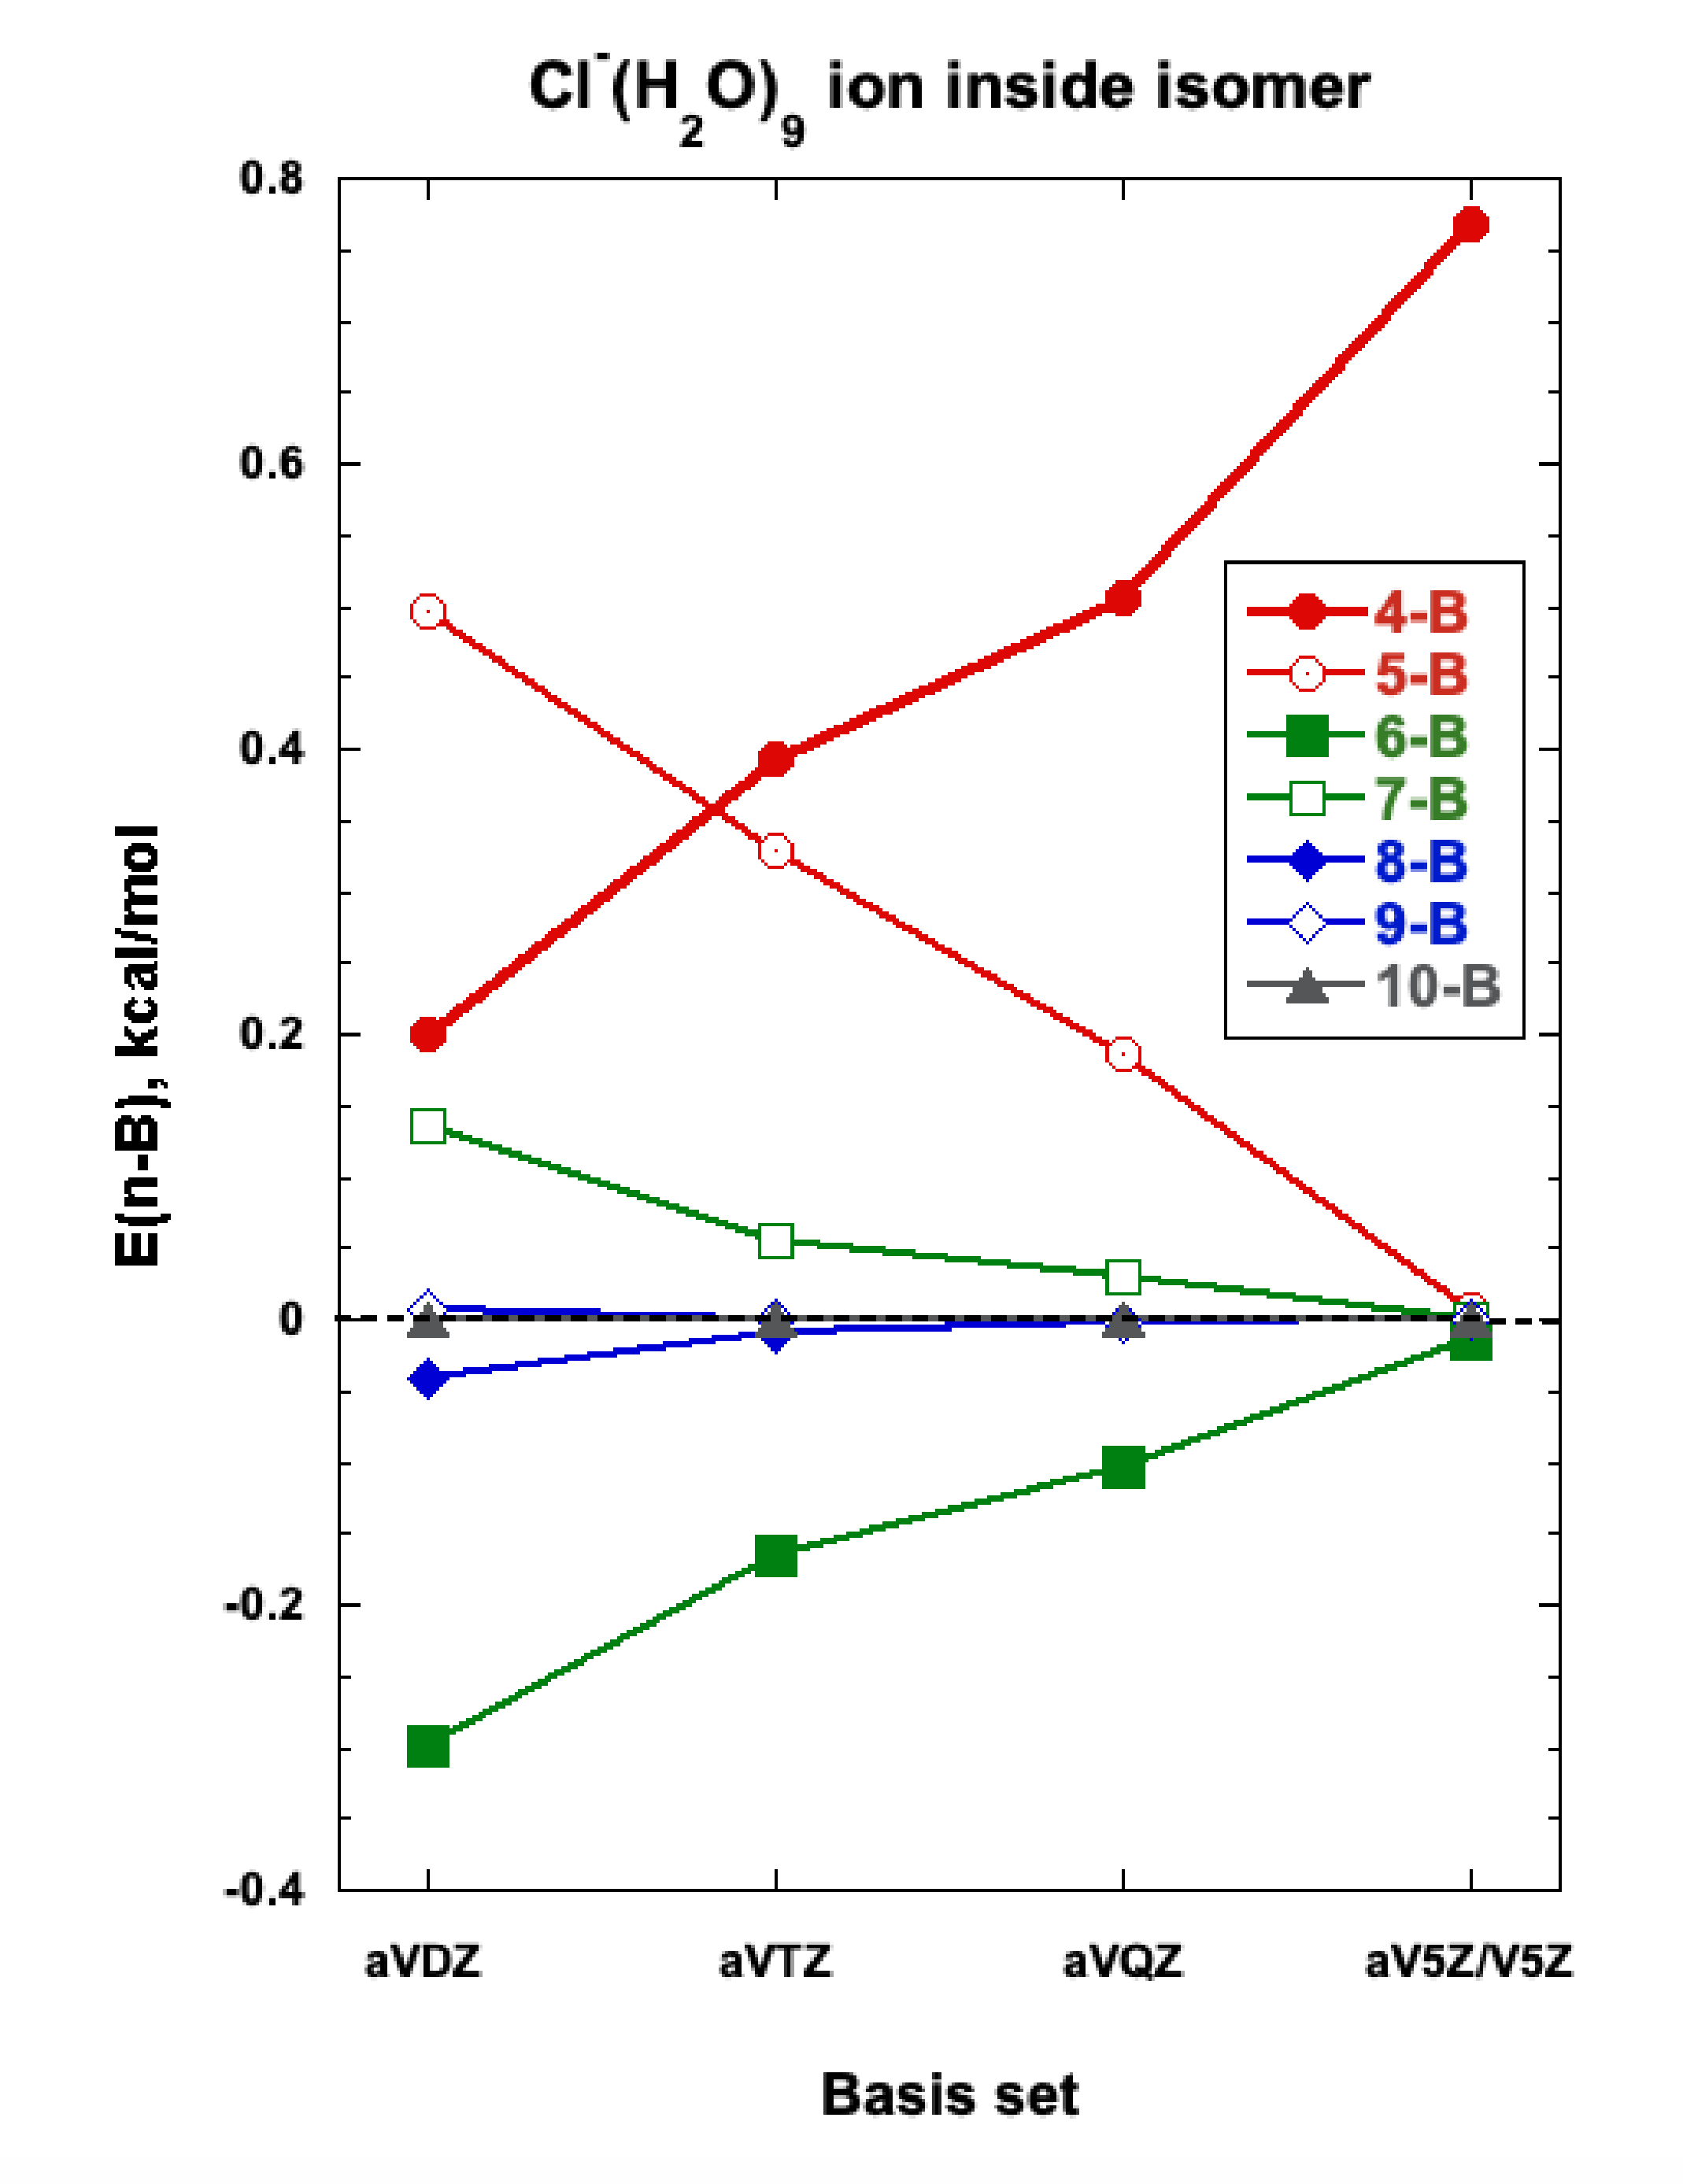
\includegraphics[width=\linewidth]{Figures/Chapter_3/figure_8_bl.pdf}
  \end{subfigure}
  \hfill
  \begin{subfigure}[t]{.5\textwidth}
    \centering
    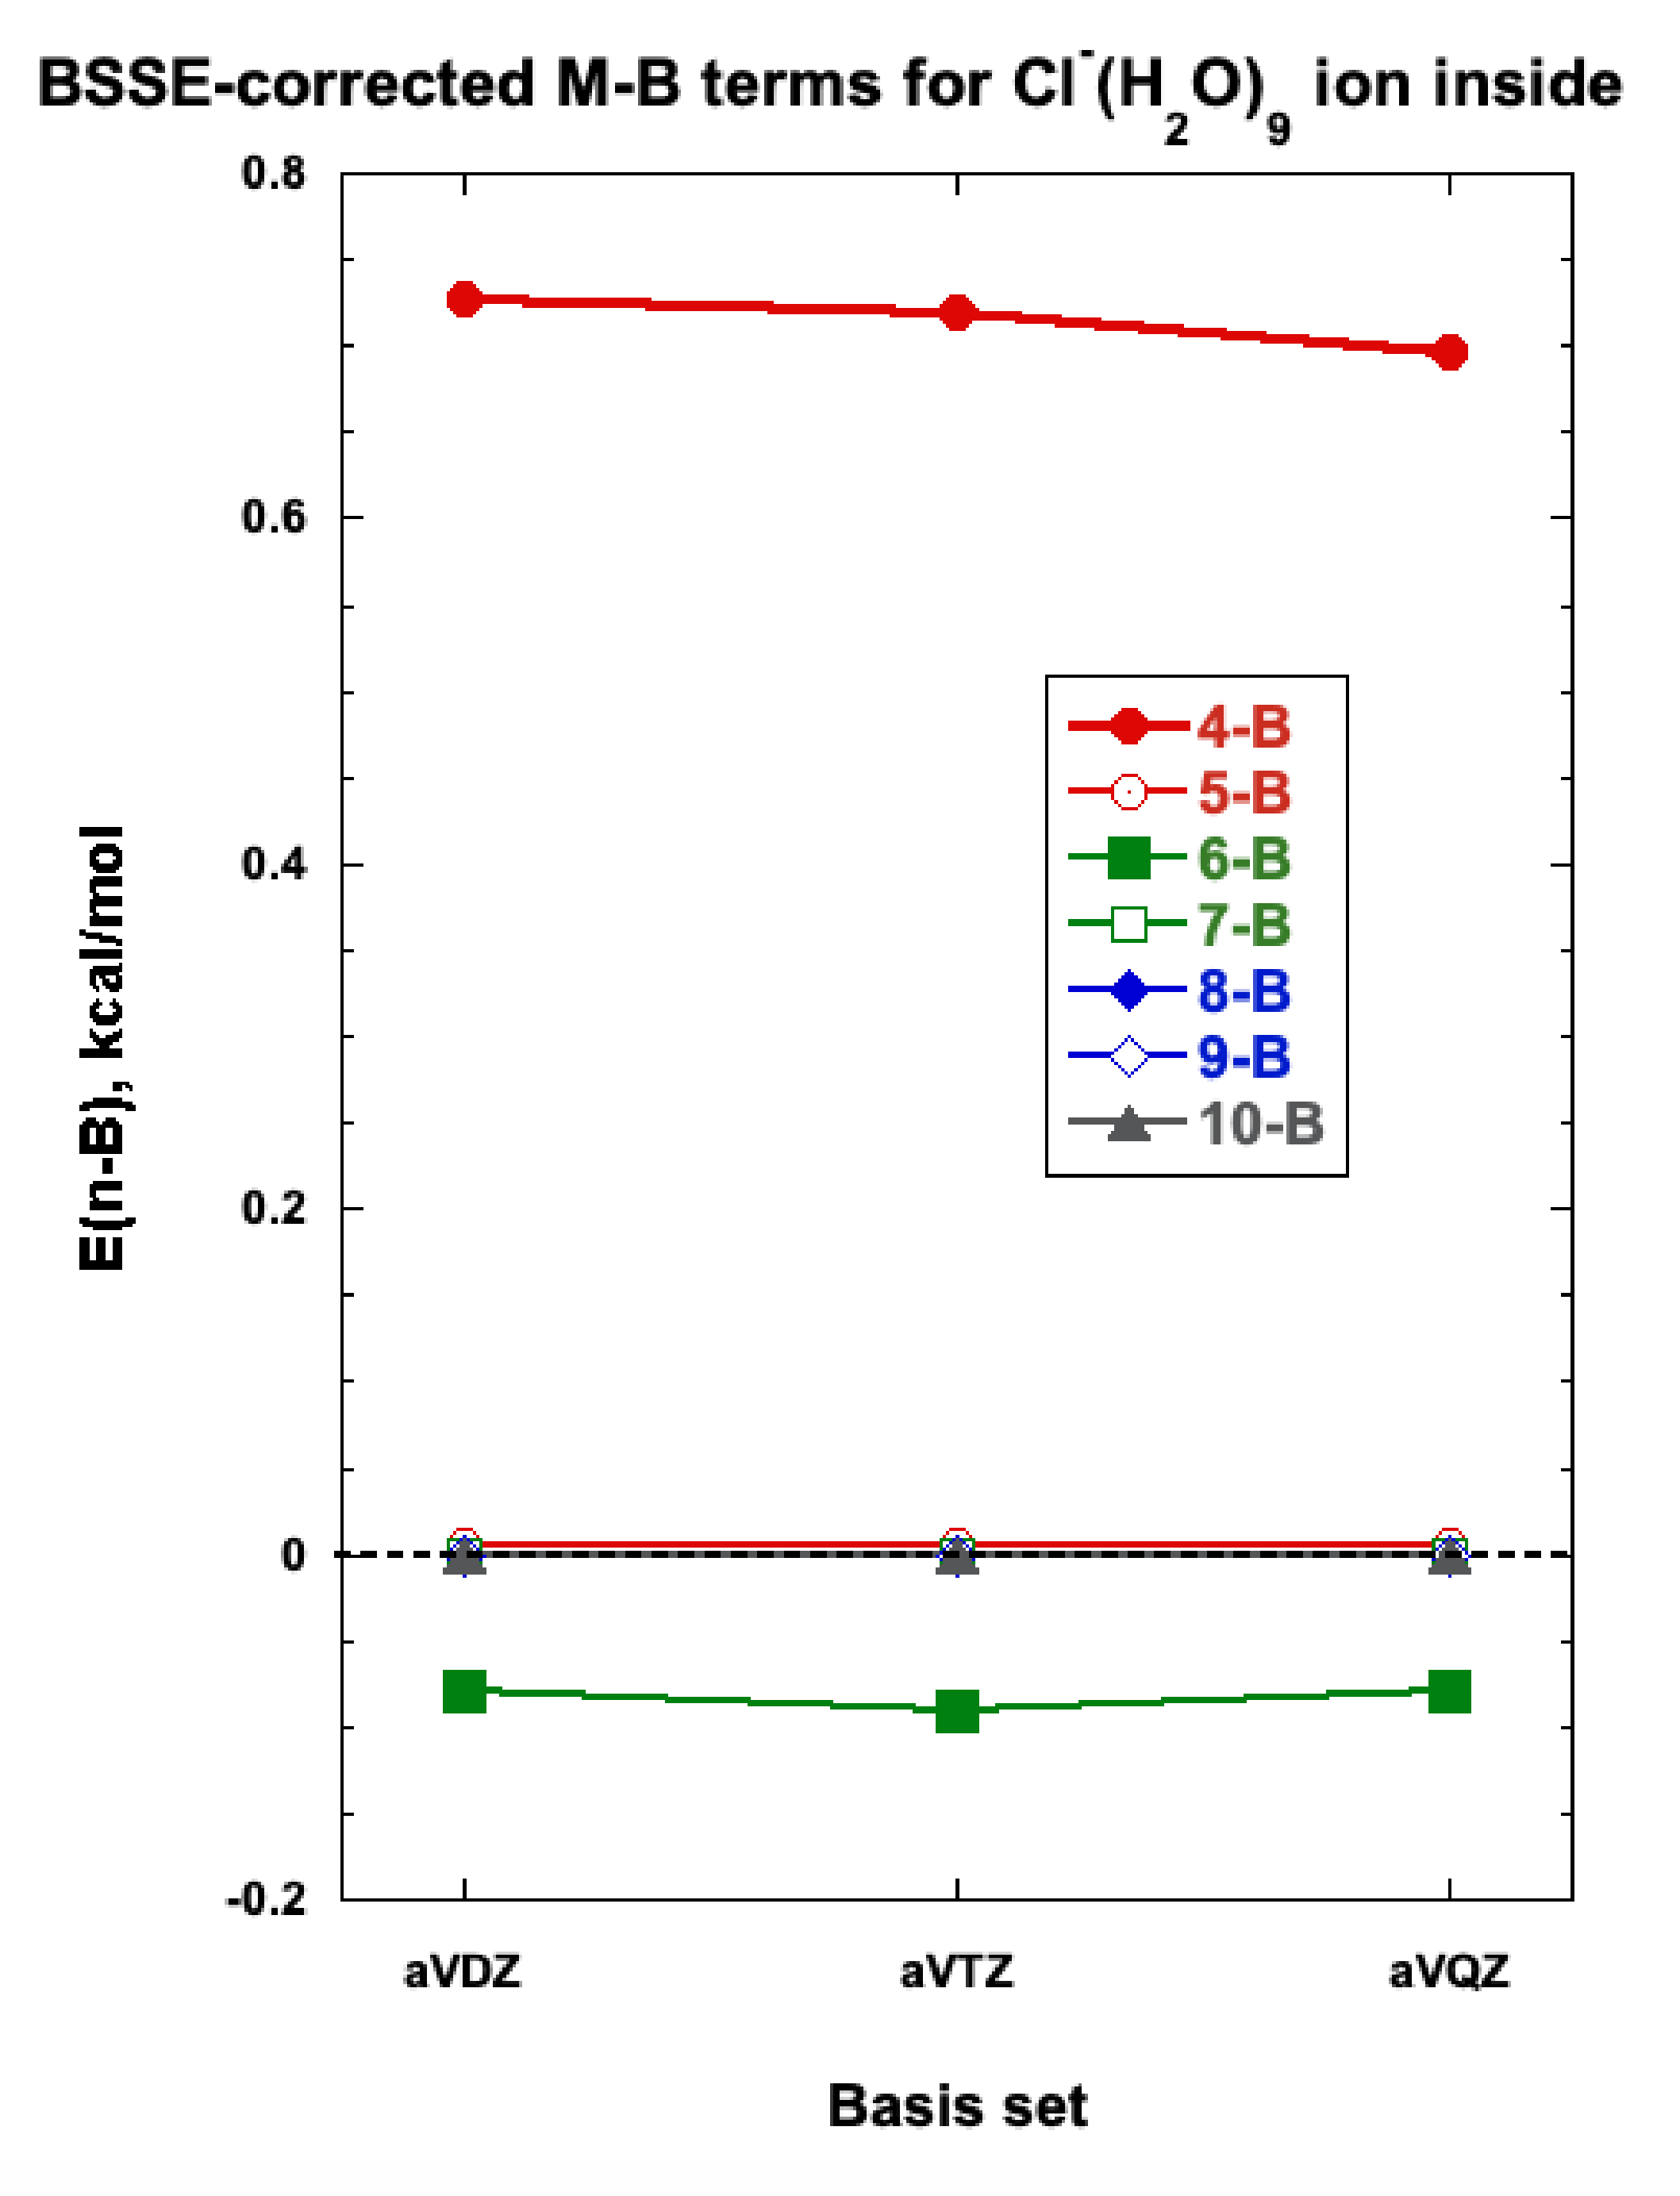
\includegraphics[width=\linewidth]{Figures/Chapter_3/figure_8_br.pdf}
  \end{subfigure}
  \caption{Many-body terms for \ce{Cl^-(H2O)9}. Notice the different y-axis scales.}
  \label{fig:MBE_II_8}
\end{figure}

\begin{figure}
  \begin{subfigure}[t]{.5\textwidth}
    \centering
    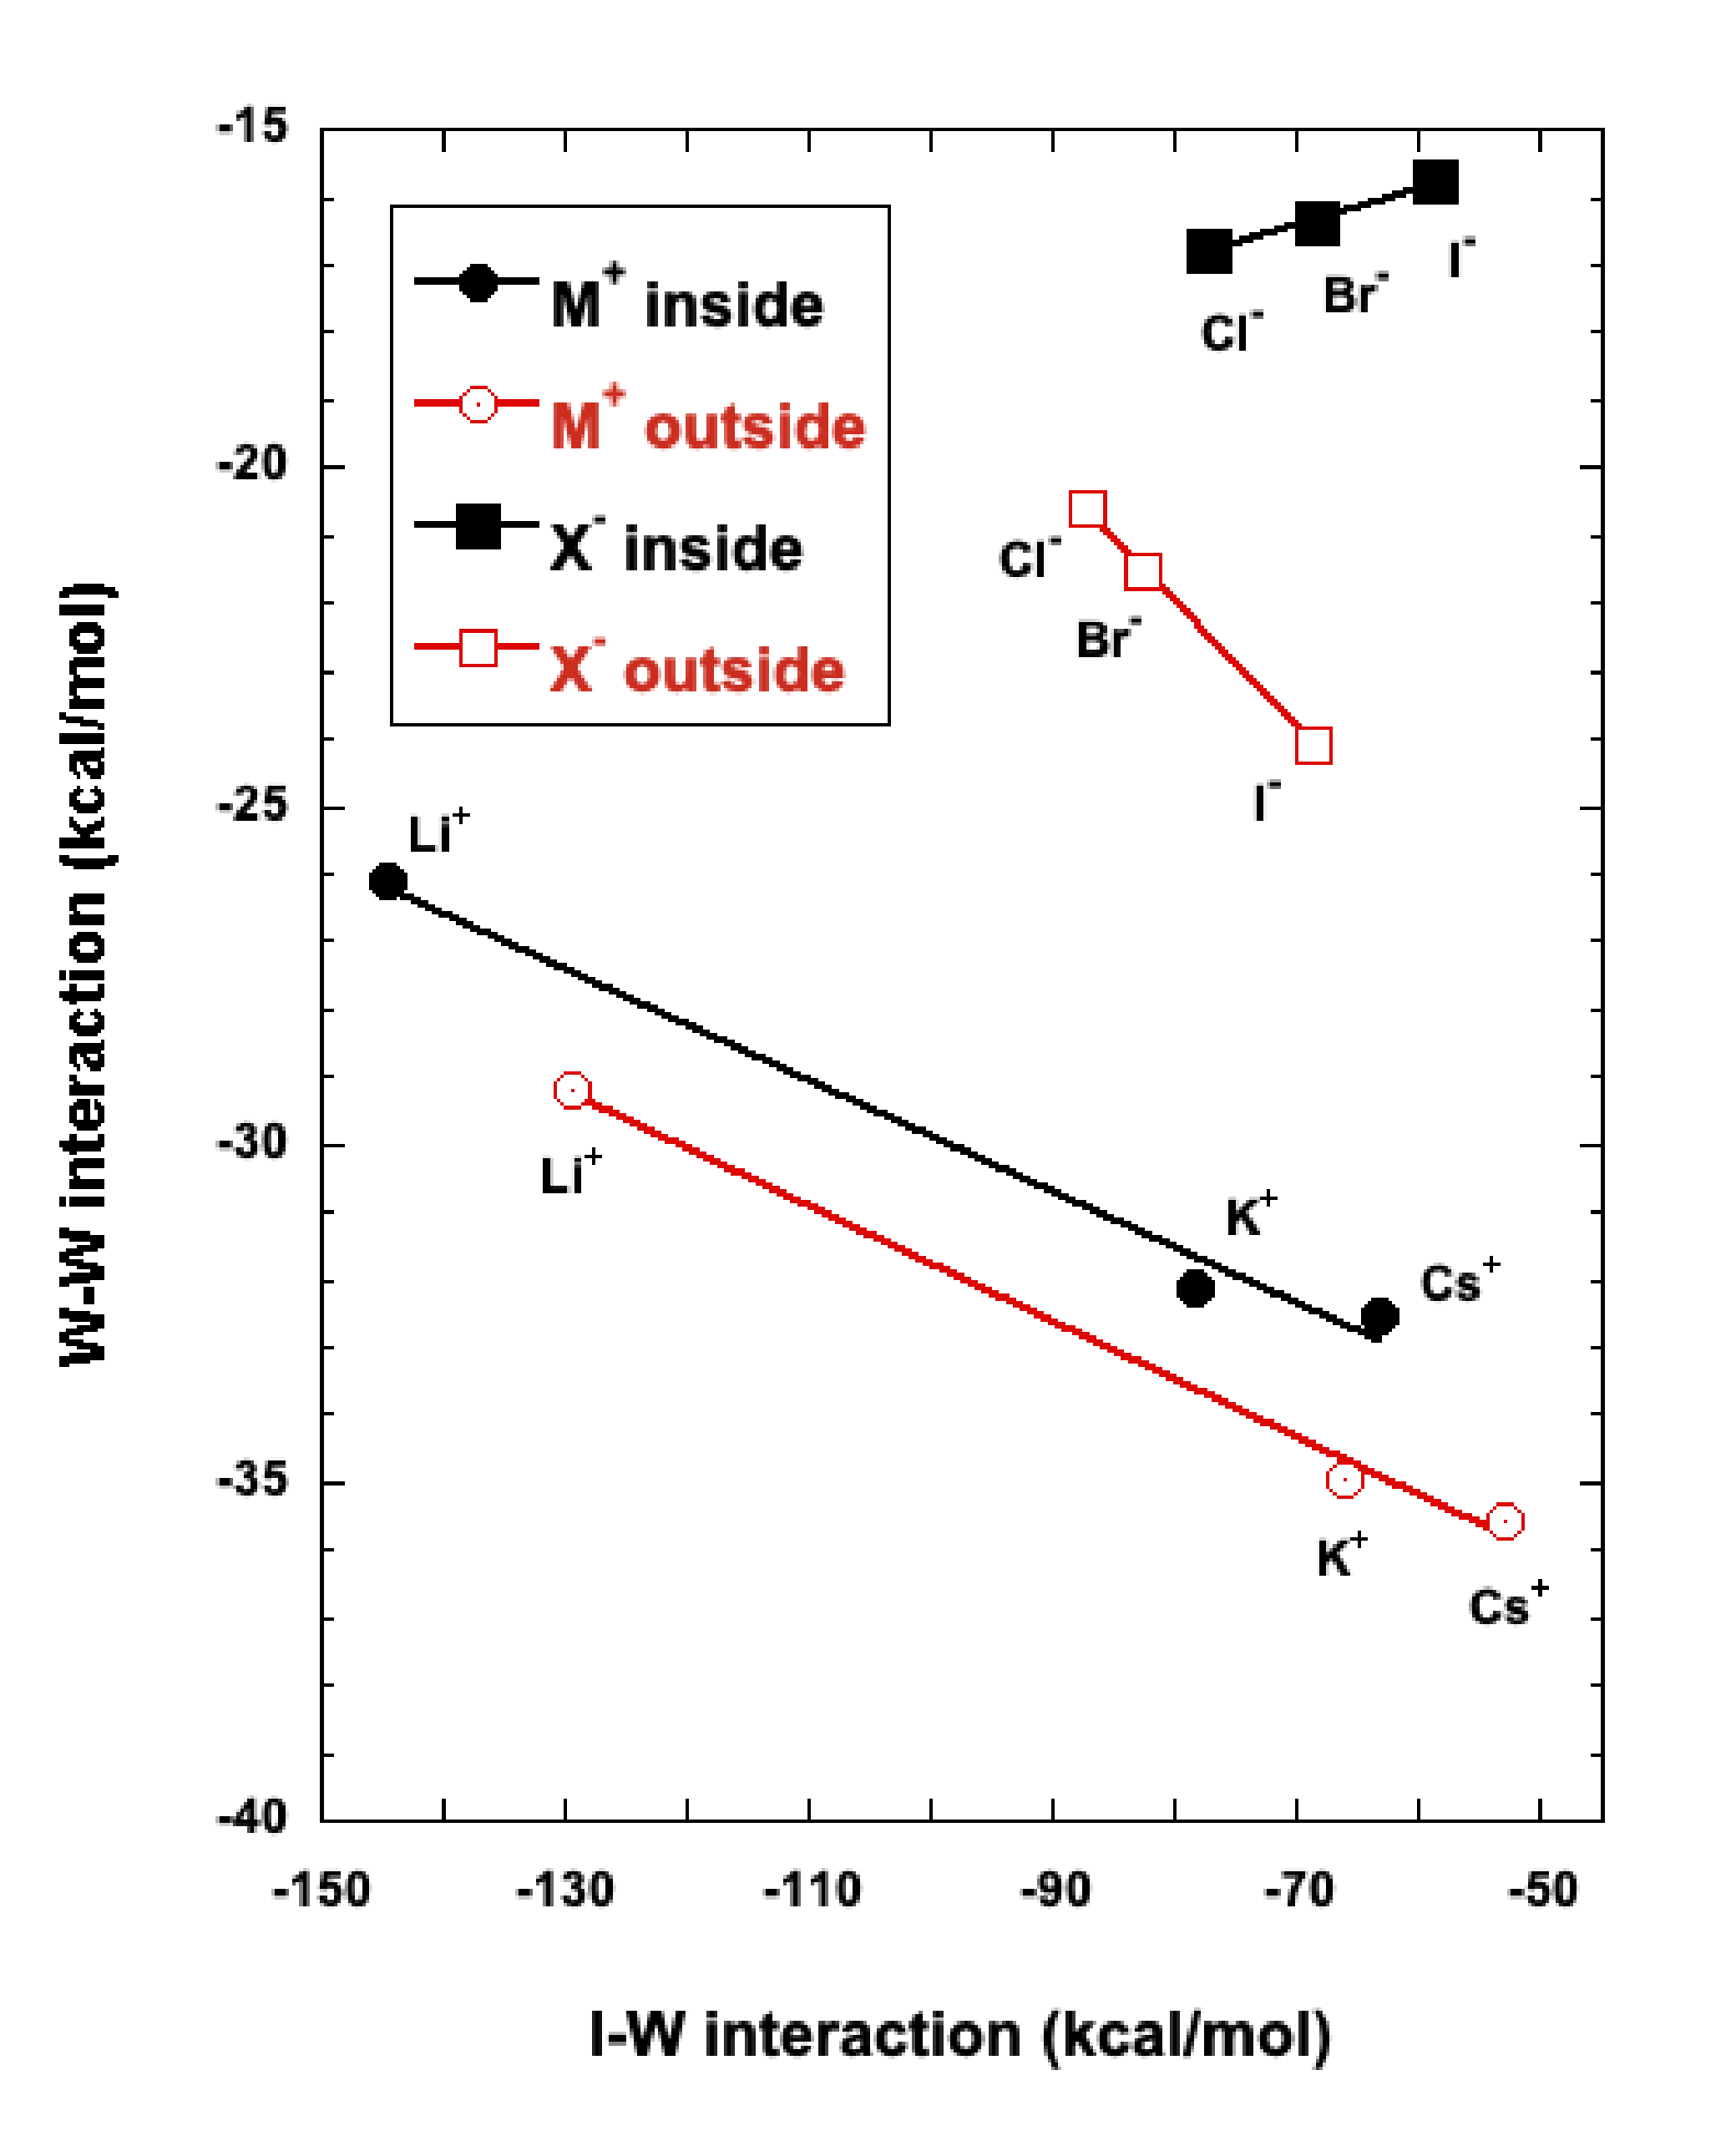
\includegraphics[width=\linewidth]{Figures/Chapter_3/figure_9_tl.pdf}
  \end{subfigure}
  \hfill
  \begin{subfigure}[t]{.5\textwidth}
    \centering
    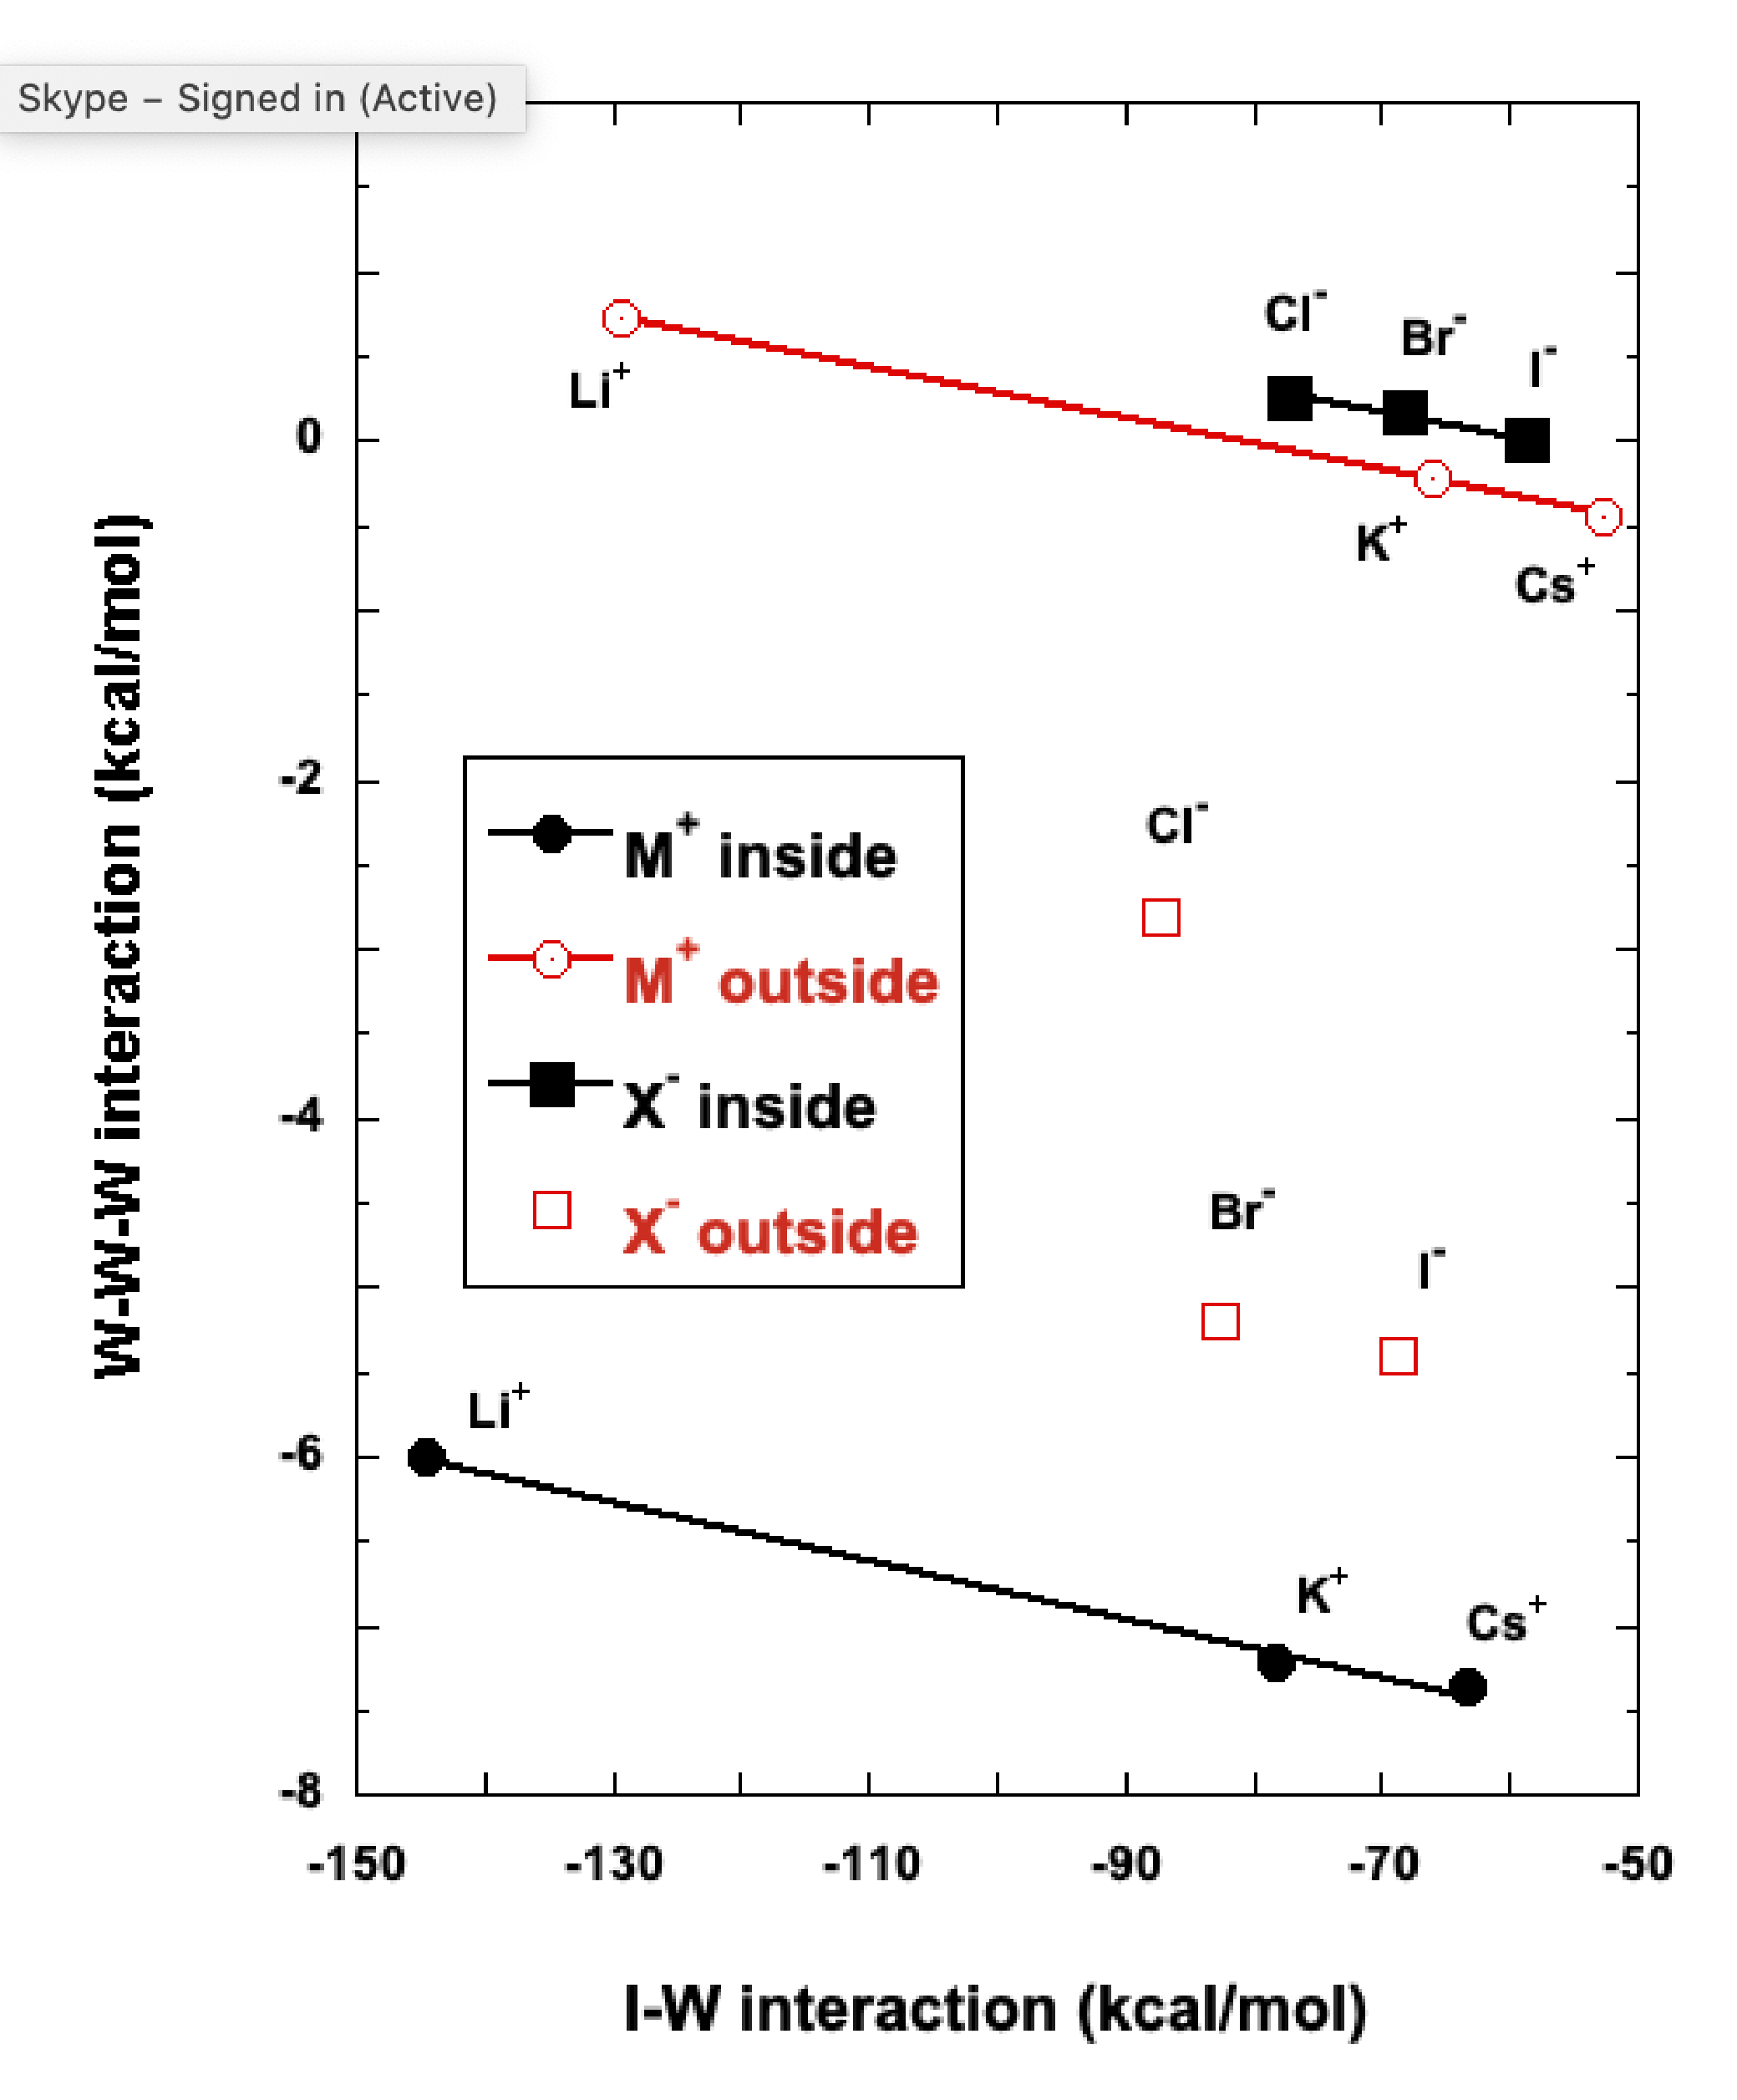
\includegraphics[width=\linewidth]{Figures/Chapter_3/figure_9_tr.pdf}
  \end{subfigure}

  \medskip

  \begin{subfigure}[t]{.5\textwidth}
    \centering
    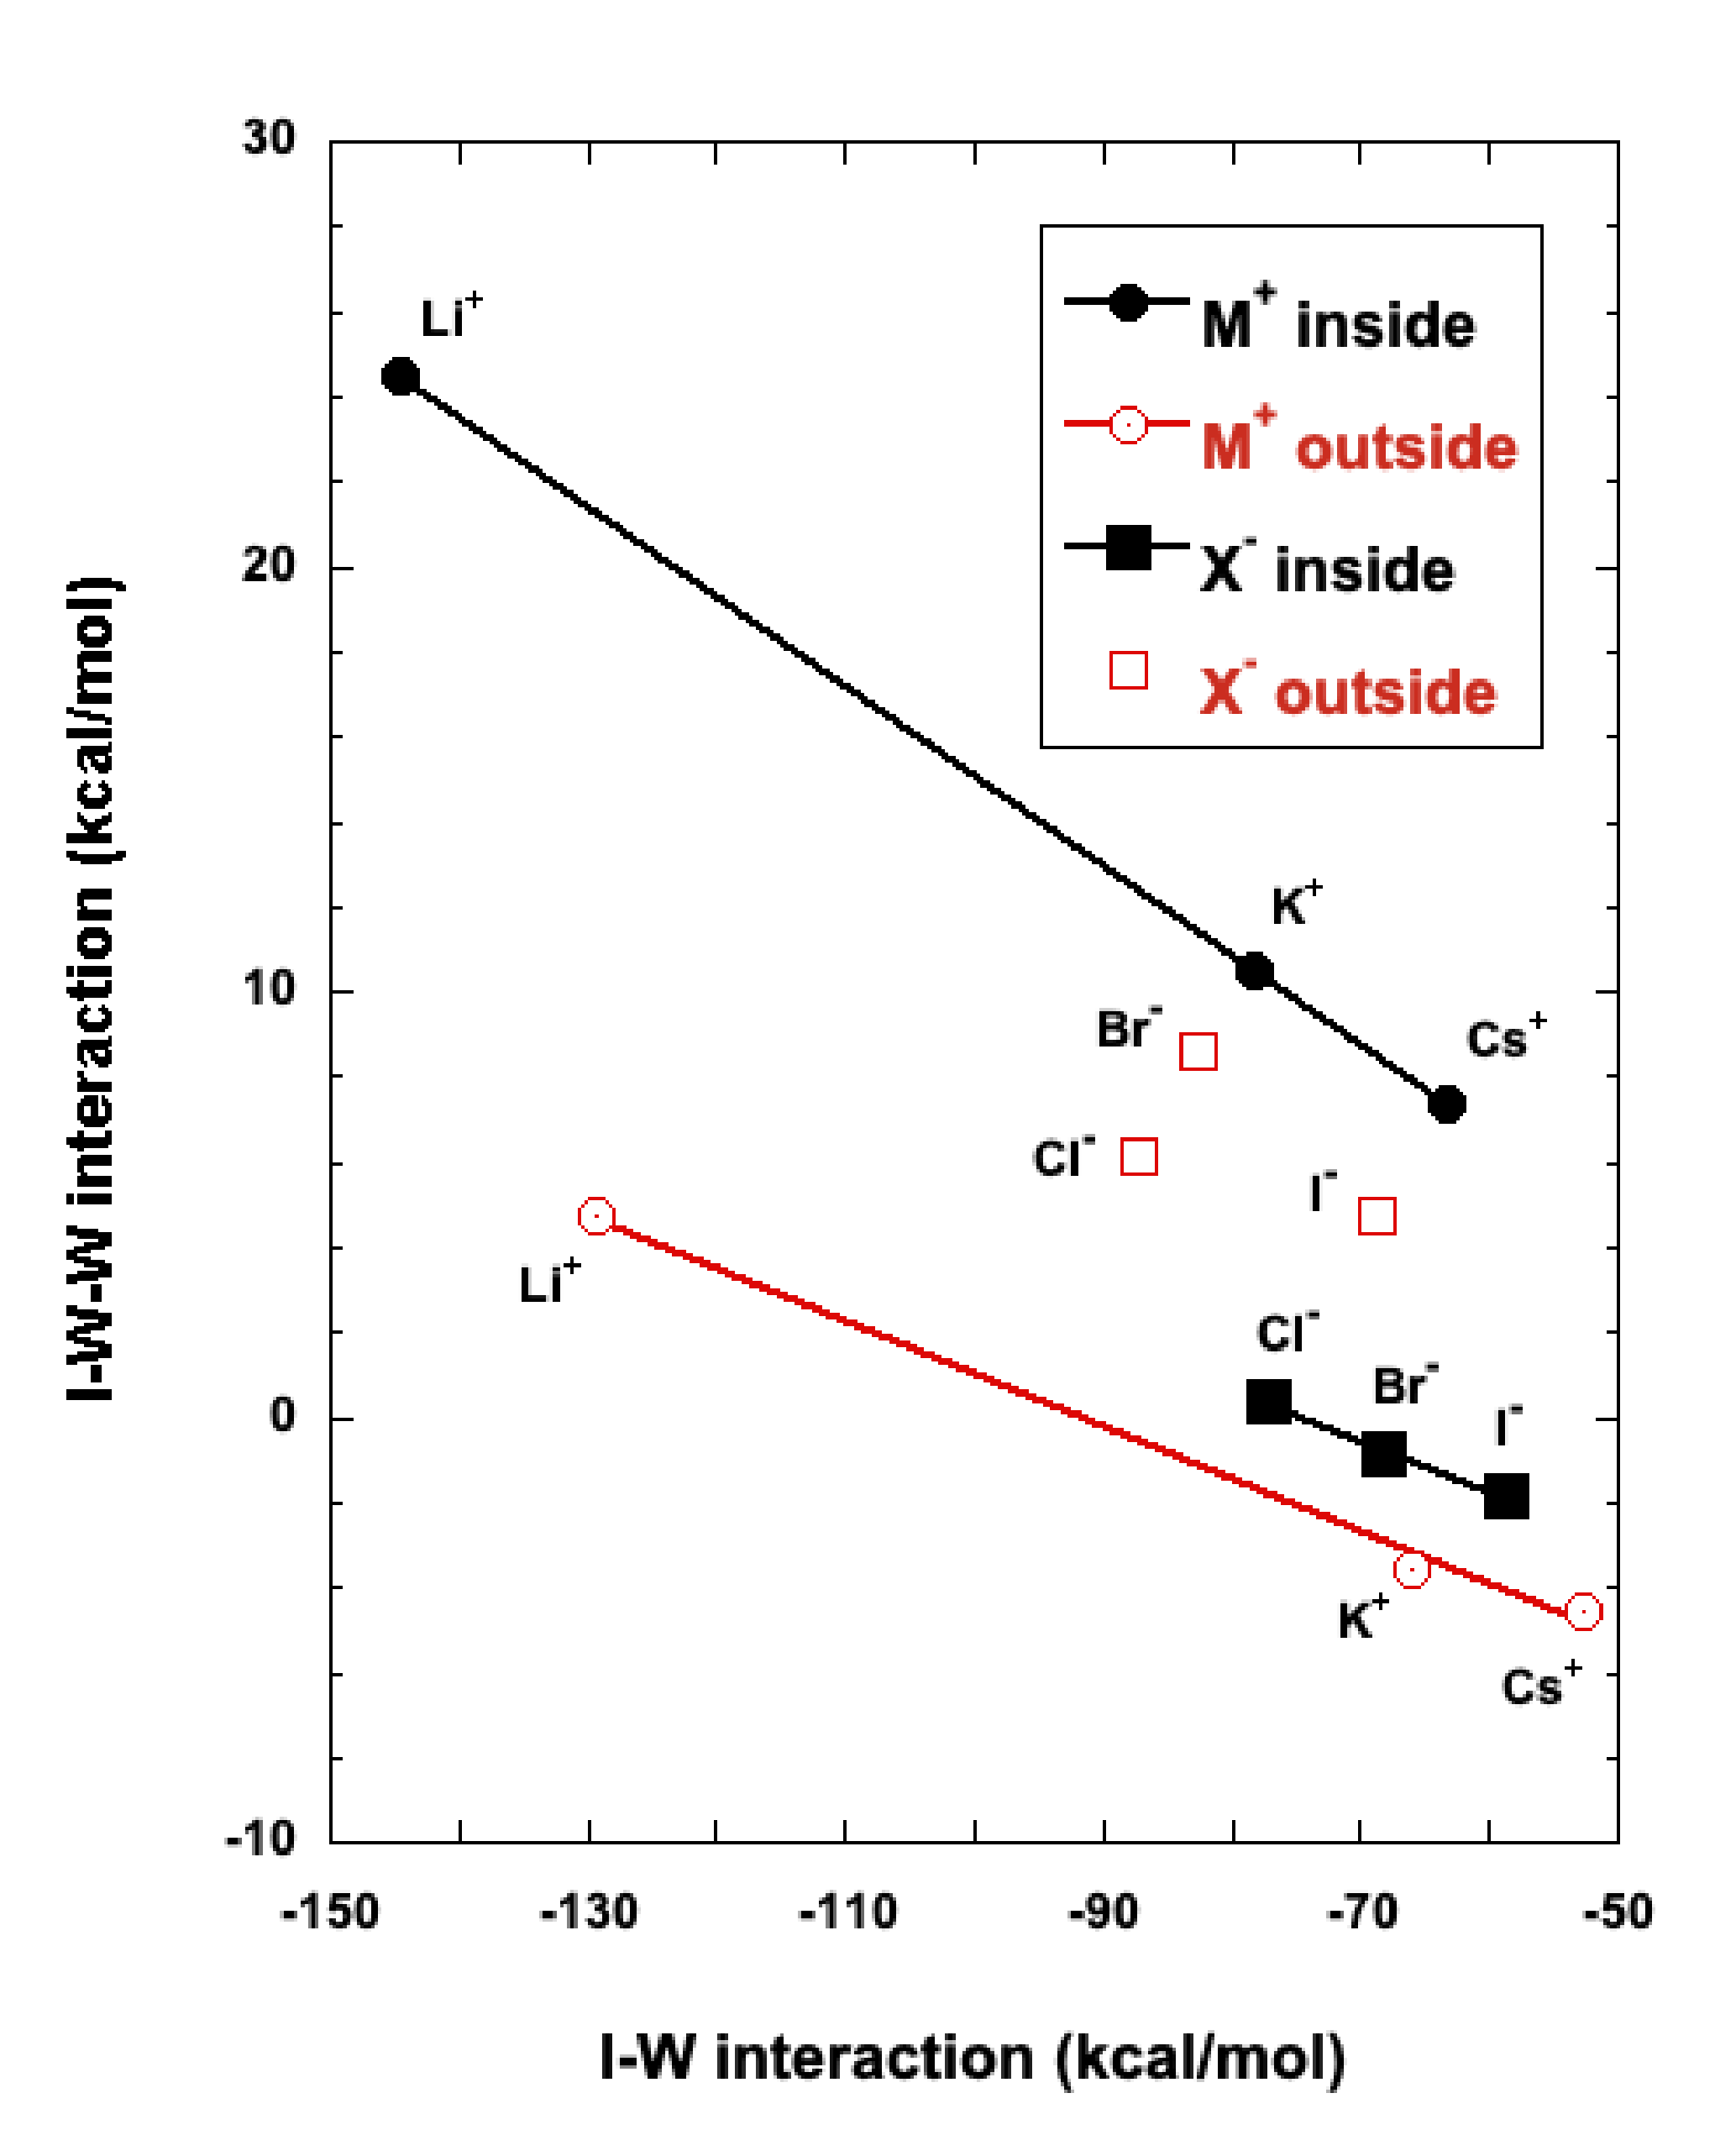
\includegraphics[width=\linewidth]{Figures/Chapter_3/figure_9_bl.pdf}
  \end{subfigure}
  \hfill
  \begin{subfigure}[t]{.5\textwidth}
    \centering
    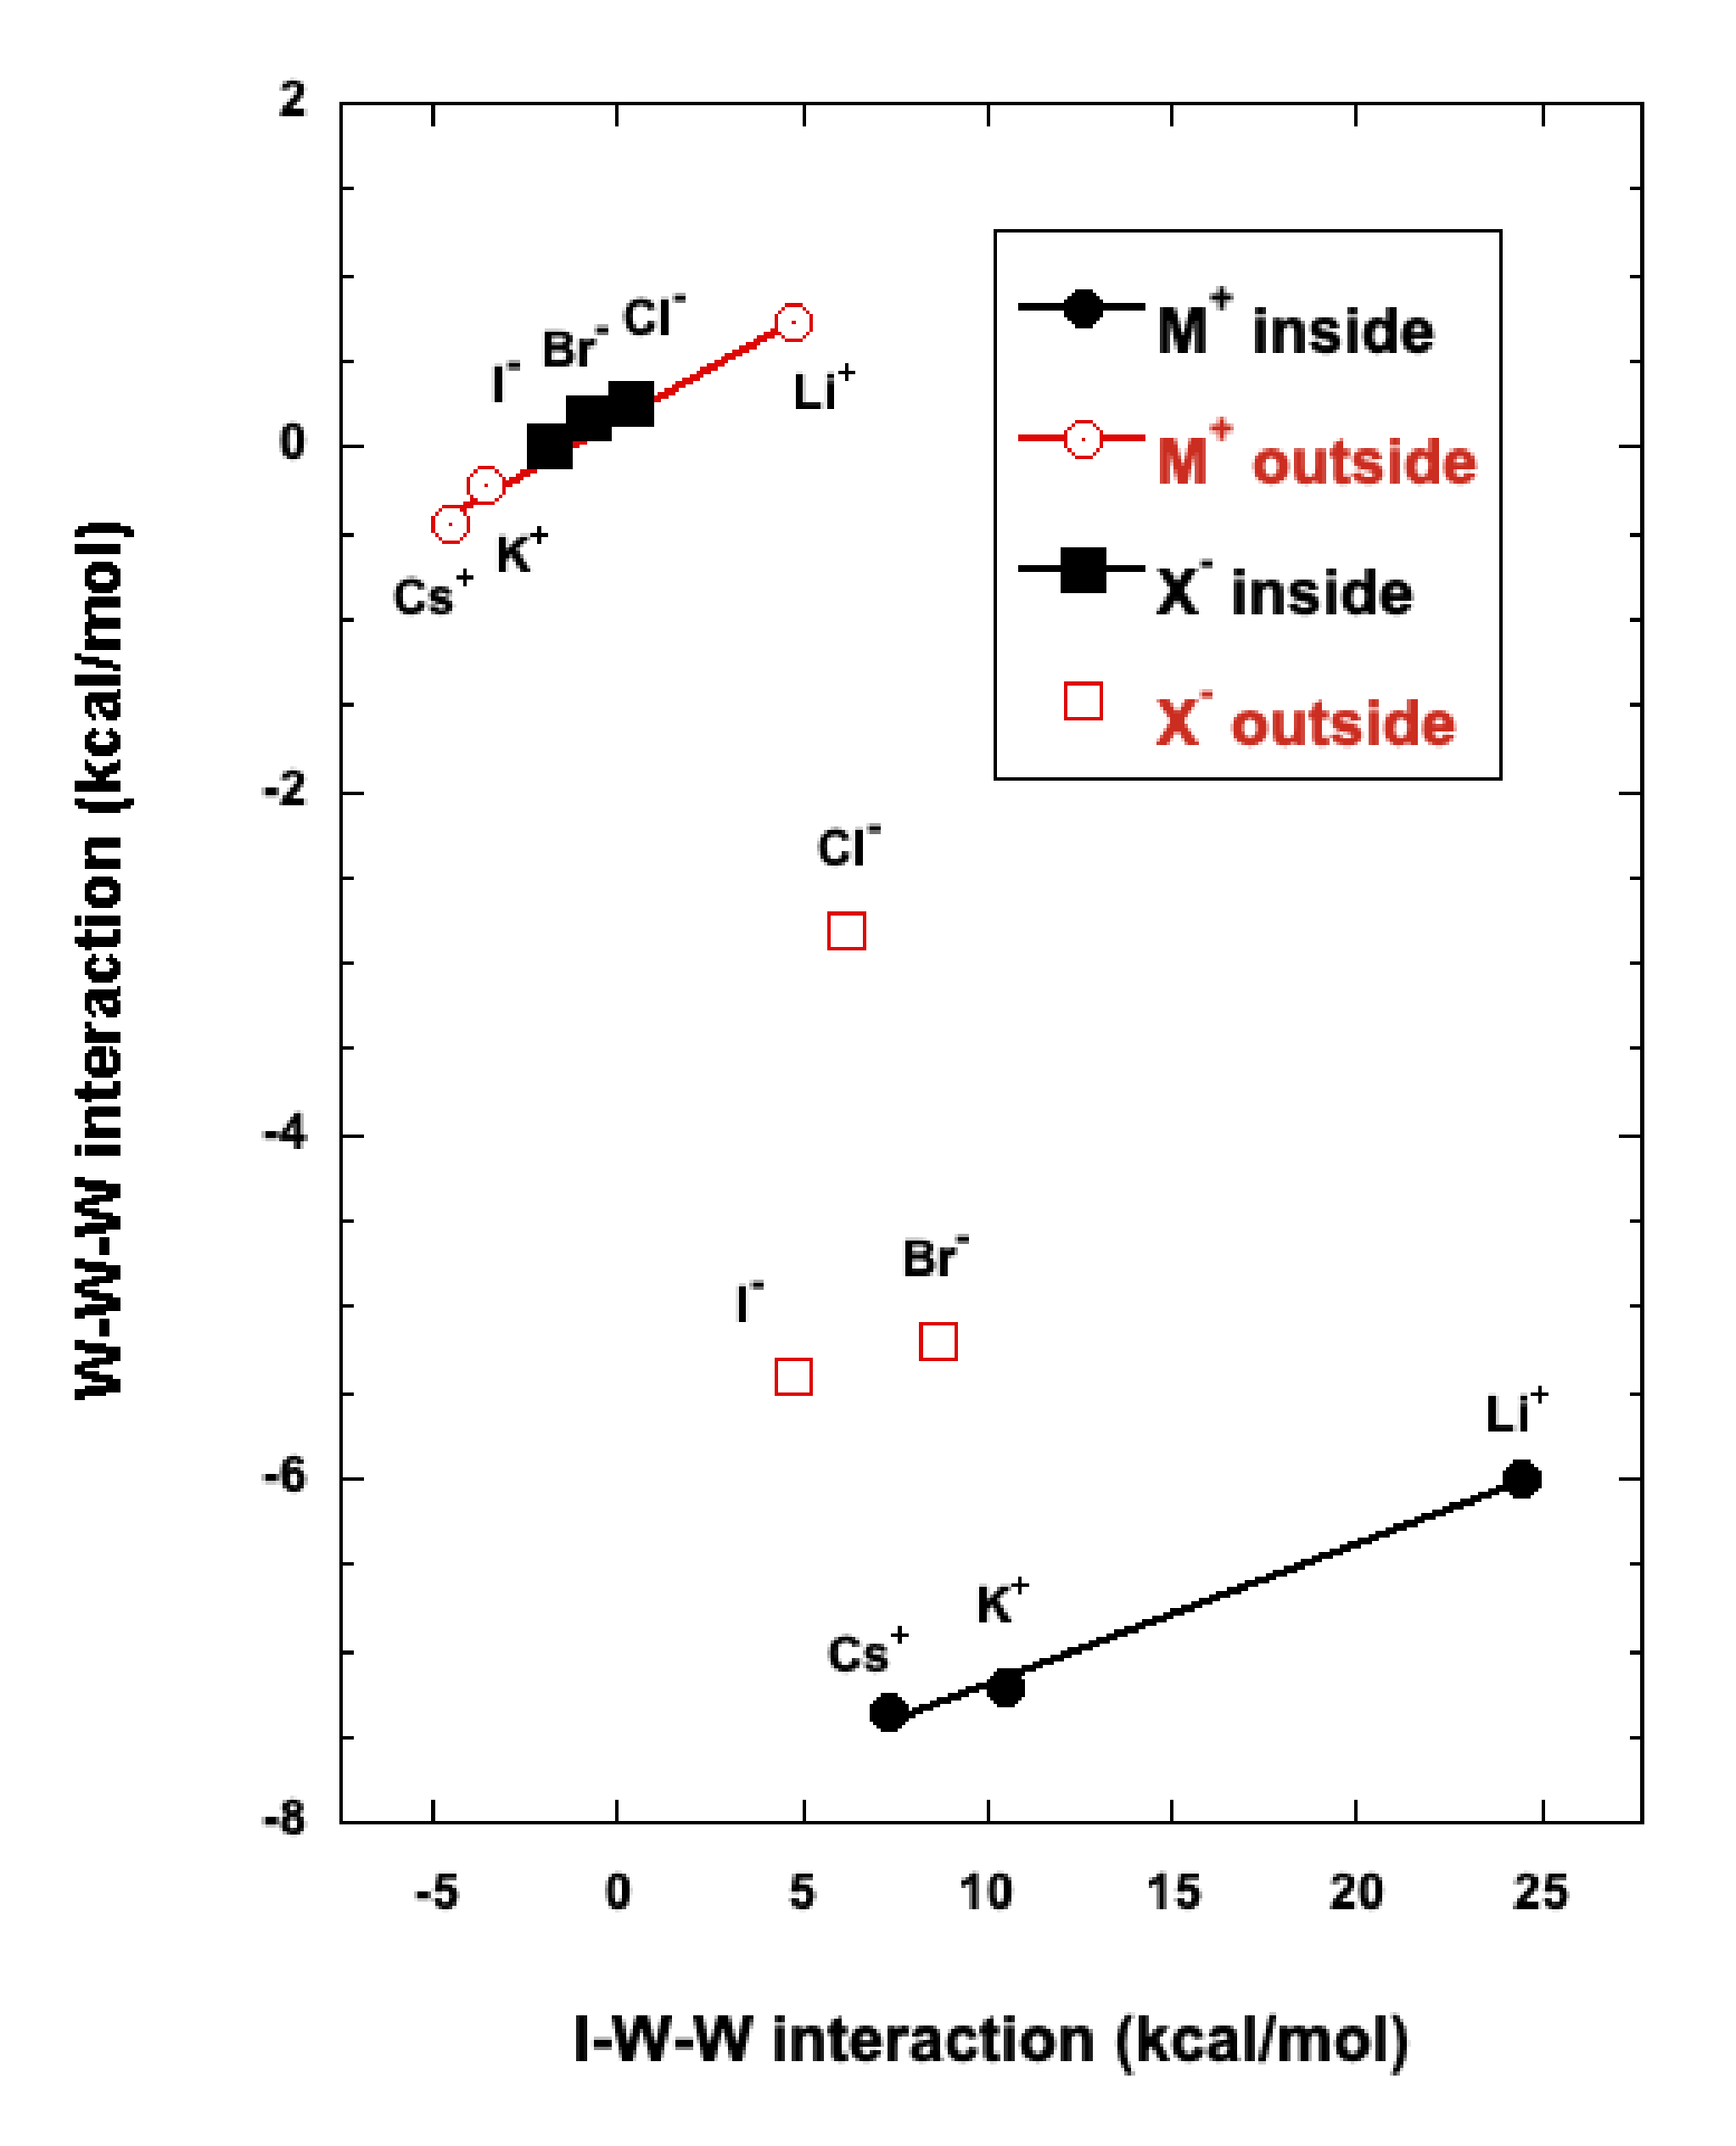
\includegraphics[width=\linewidth]{Figures/Chapter_3/figure_9_br.pdf}
  \end{subfigure}
  \caption{Correlations between the various interactions for the \ce{Z^{+/-}(H2O)9}, \ce{Z} = \ce{M^+} (\ce{Li^+}, \ce{K^+}, \ce{Cs^+}) and \ce{Z} = \ce{X^-} (\ce{Cl^-}, \ce{Br^-}, \ce{I^-}) clusters. (a) Top left panel: (W-W) vs. (I-W), (b) top right panel: (W-W-W) vs. (I-W), (c) bottom left panel: (I-W-W) vs. (I-W) and (d) bottom right panel: (I-W-W) vs. (W-W-W) interactions.}
  \label{fig:MBE_II_9}
\end{figure}

\begin{figure}[t]
\uwsinglespace
\centering
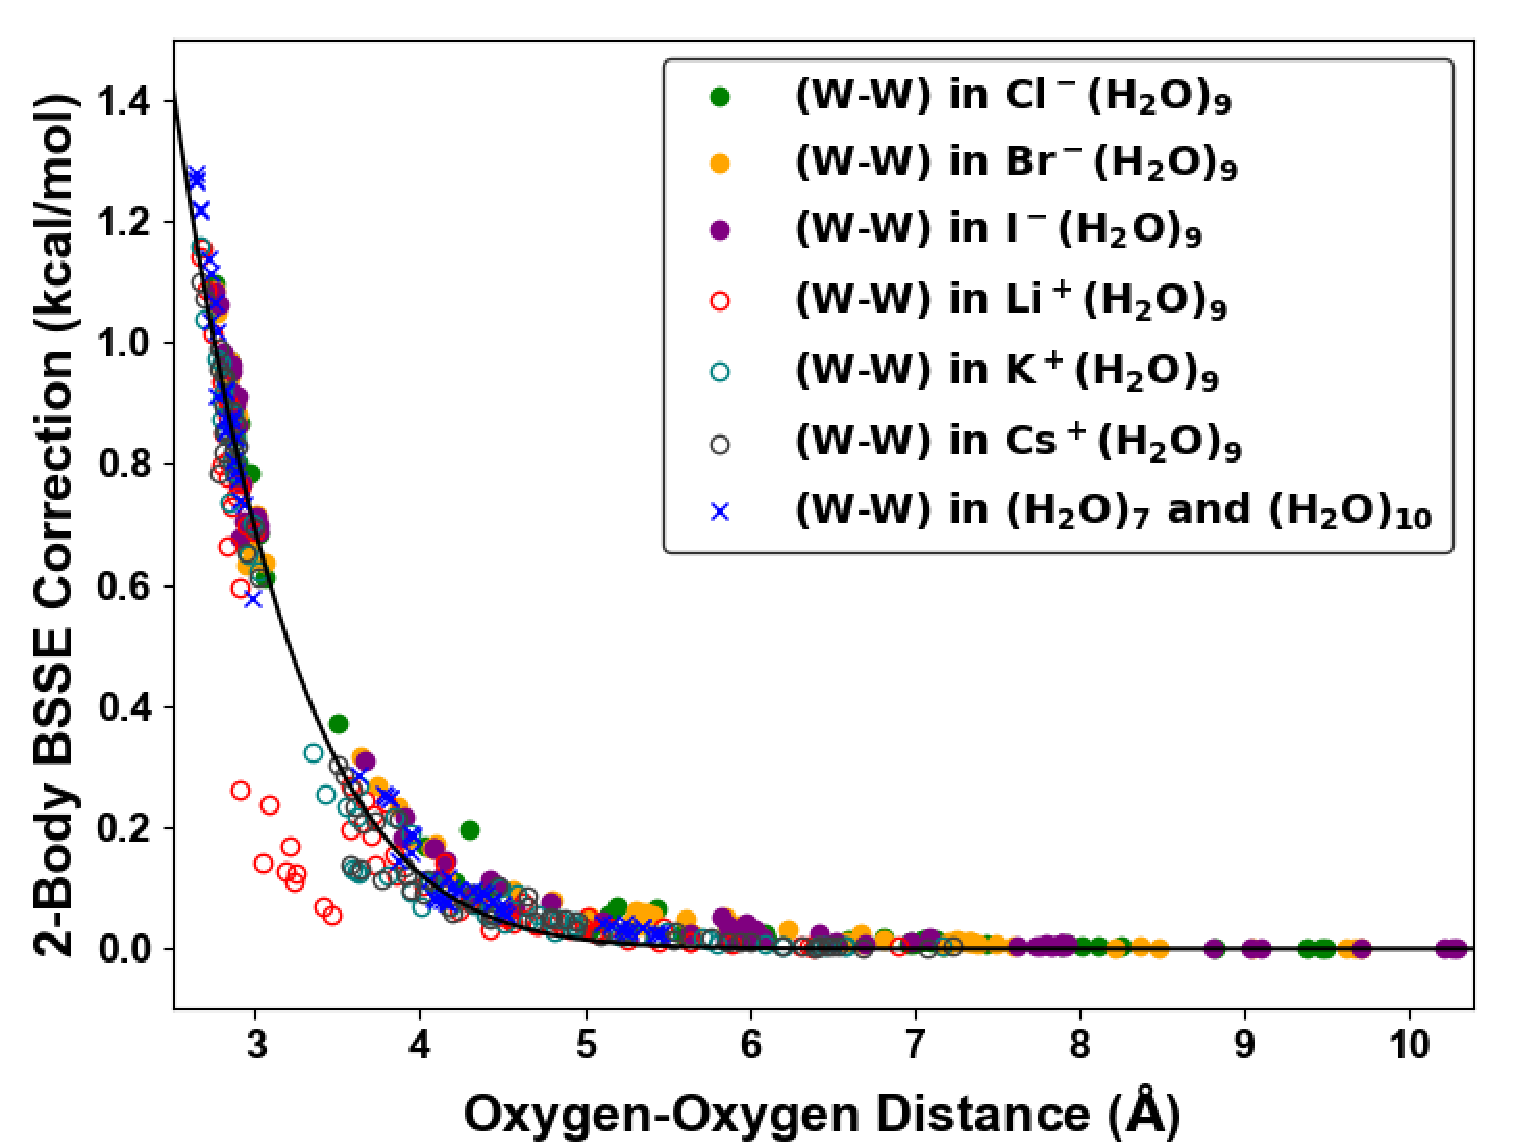
\includegraphics[width=\textwidth]{Figures/Chapter_3/figure_10.pdf}
\caption[temp]{2-Body BSSE correction for all 498 water dimers extracted from the \ce{Z^{+/-}(H2O)9}, \ce{Z} = \ce{Li^+}, \ce{K^+}, \ce{Cs^+}, \ce{Cl^-}, \ce{Br^-}, \ce{I^-}, clusters as well as the two neutral water clusters \ce{(H2O)7} and \ce{(H2O)_{10}} as a function of the Oxygen – Oxygen distance. The solid line represents a fit to the function $BSSE(R_{ij})=A[1+erf(-BR_{ij})]$ yielding the parameters $A = 13.346$ and $B = 0.457$. The water dimers extracted from the two isomers of the \ce{Li^+(H2O)9} clusters were not included in the fit. See text for details.}
\label{fig:MBE_II_10}
\end{figure}

\begin{figure}[t]
\uwsinglespace
\centering
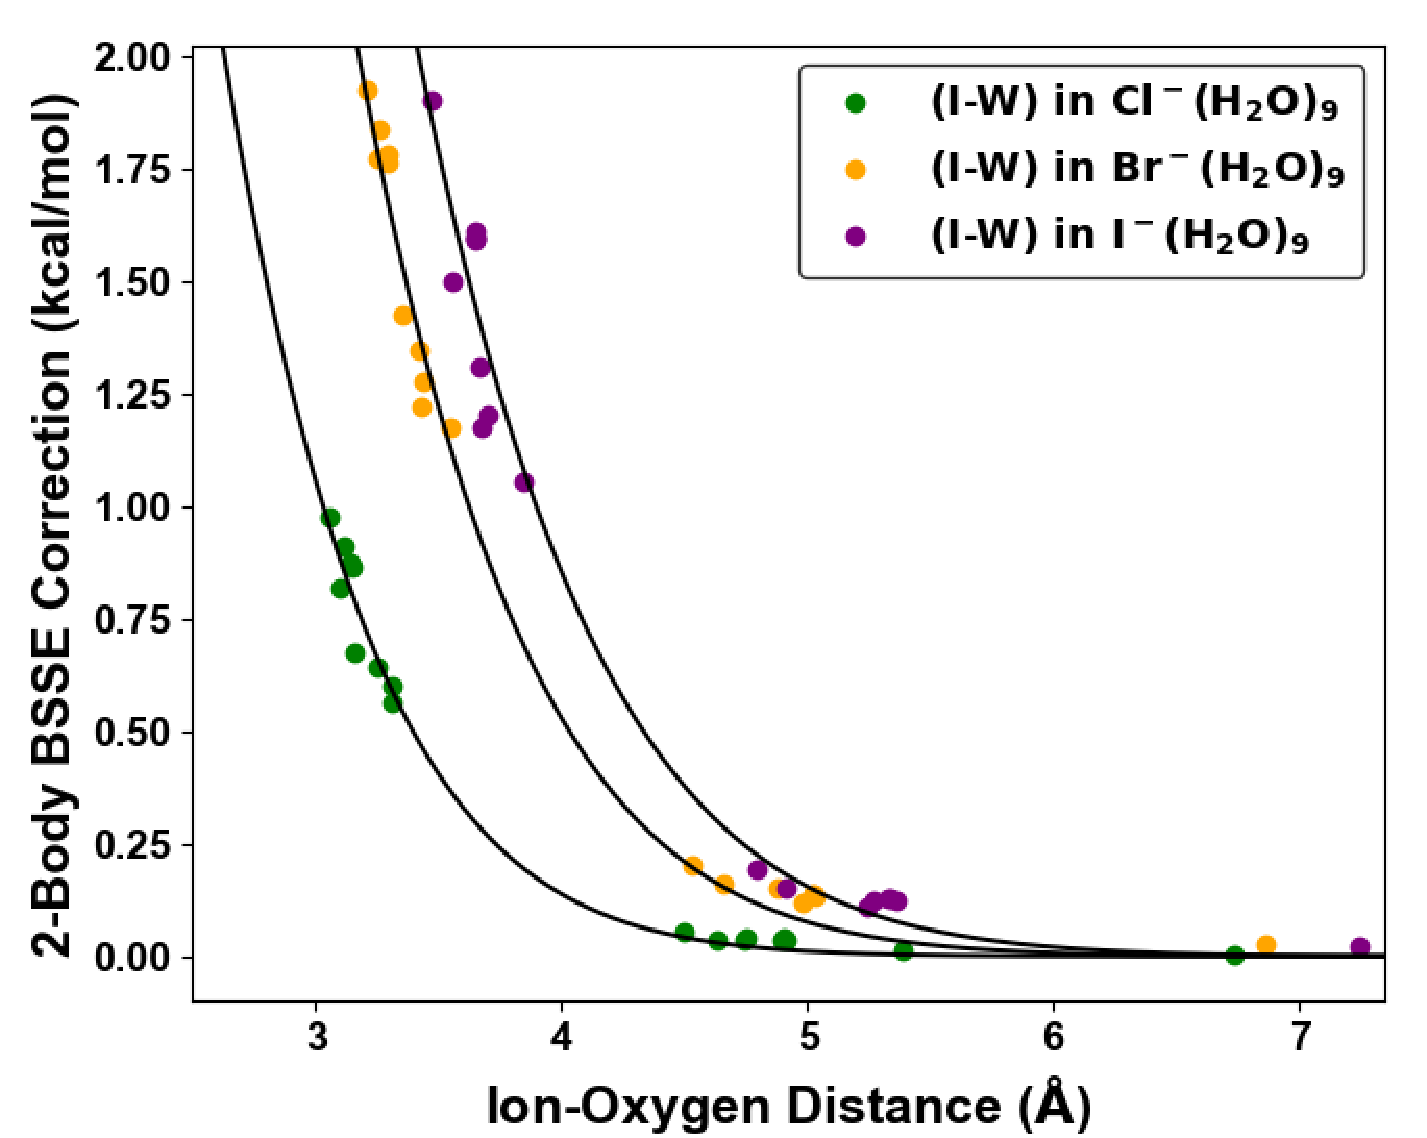
\includegraphics[width=\textwidth]{Figures/Chapter_3/figure_11.pdf}
\caption[temp]{2-B BSSE correction for all 54 ion - water dimers extracted from the \ce{Z-(H2O)9}, where \ce{Z} = \ce{Cl^-}, \ce{Br^-}, \ce{I^-}, clusters. The solid lines represents fits to the function $BSSE(R_{ij})=A[1+erf(-BR_{ij})]$ yielding the parameters  $A_{\ce{F^-}} = 12.161$, $B_{\ce{F^-}} = 0.469$; $A_{\ce{Cl^-}} = 33.831$, $B_{\ce{Cl^-}} =0.507$; $A_{\ce{Br^-}} = 42.159$, $B_{\ce{Br^-}} = 0.441$; $A_{\ce{I^-}} = 43.118$, $B_{\ce{I^-}} = 0.412$.}
\label{fig:MBE_II_11}
\end{figure}

\begin{figure}[t]
\uwsinglespace
\centering
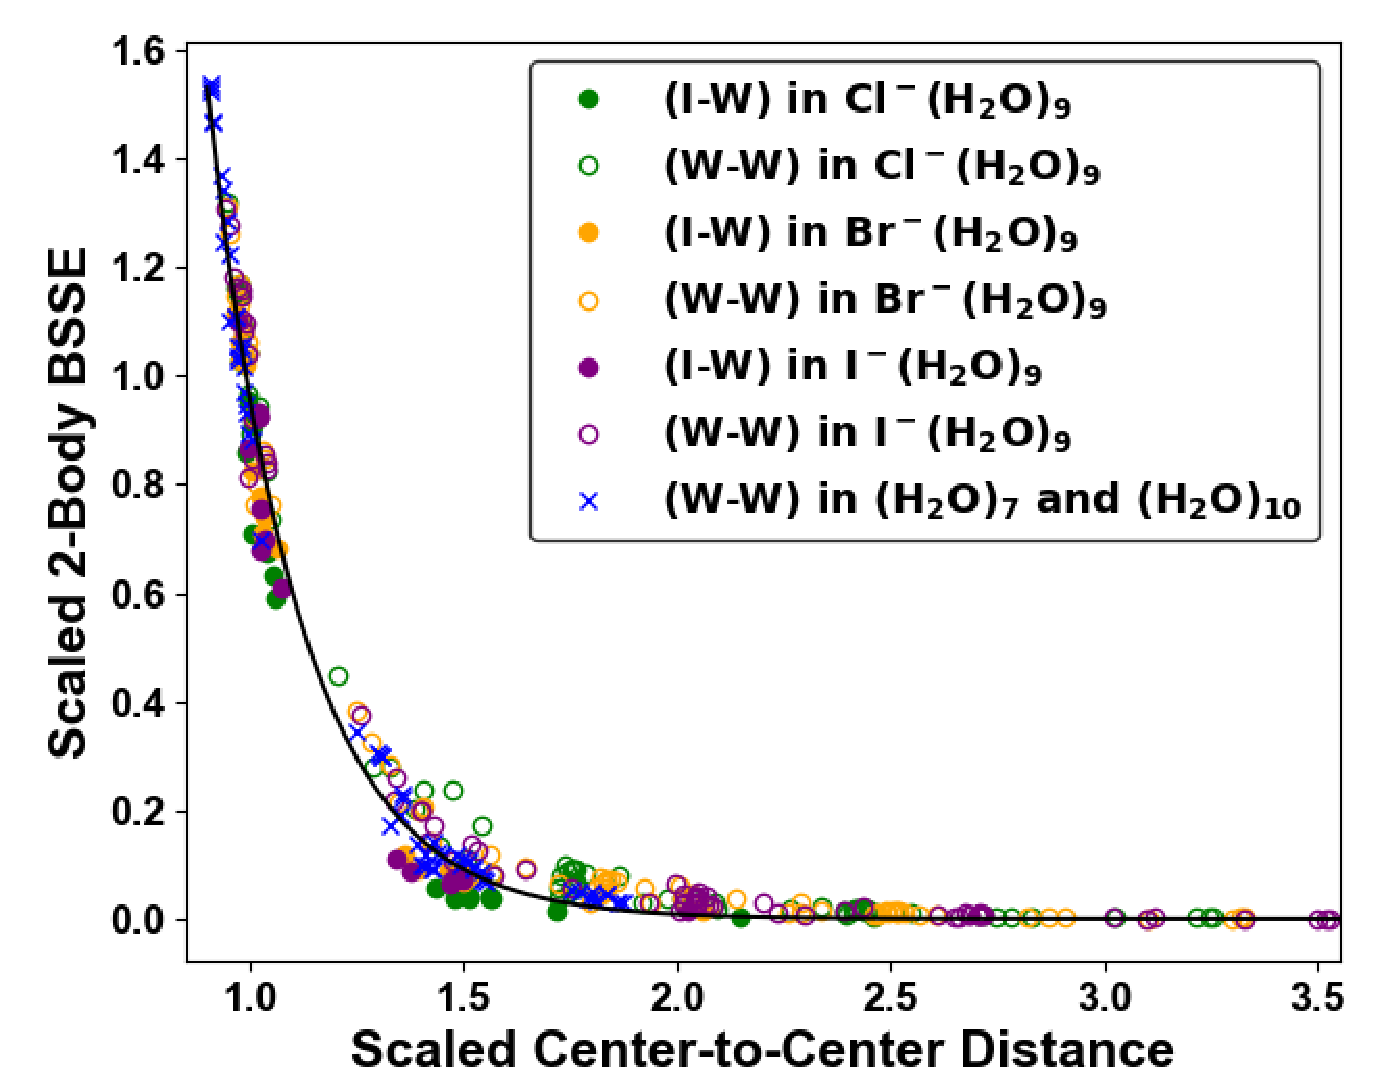
\includegraphics[width=\textwidth]{Figures/Chapter_3/figure_12.pdf}
\caption[temp]{Scaled 2-Body BSSE values for all 336 ion-water and water-water dimers cut from \ce{Z^-(H2O)9} where \ce{Z} = \ce{Cl^-}, \ce{Br^-}, and \ce{I^-} as well as two neutral water clusters of \ce{(H2O)7} and \ce{(H2O)_{10}}. Each energy is scaled by the size of the BSSE-correction of the corresponding \ce{Z^-(H2O)} dimer or that of a neutral water dimer. Each distance is scaled by the equilibrium center-to-center distance in those same dimers. See text for more detail.}
\label{fig:MBE_II_12}
\end{figure}

\end{document}
